\documentclass[11pt]{article}
\usepackage{units}
\usepackage[small, bf]{caption}
\usepackage[numbers,sort&compress]{natbib}
\usepackage{color}
\usepackage{amssymb, amsmath}
\usepackage{graphicx}
\usepackage{epstopdf}
\usepackage{verbatim}
\usepackage{amsfonts}
\usepackage{subfloat}
\usepackage{subfig}
\usepackage{multirow}
\usepackage{authblk}
\usepackage{array}
\usepackage{footmisc}
\usepackage{tabularx}
\usepackage{sidecap}
\usepackage{setspace}
\usepackage[normalem]{ulem}
\usepackage{pgfplotstable}
\usepackage[margin=1in]{geometry}
\renewcommand\Affilfont{\small}
\newcommand{\ignore}[1]{}
\usepackage{float}

\newenvironment{packed_enum}{
\begin{enumerate}
  \setlength{\itemsep}{1pt}
  \setlength{\parskip}{0pt}
  \setlength{\parsep}{0pt}
}{\end{enumerate}}
\newenvironment{packed_itemize}{
\begin{itemize}
  \setlength{\itemsep}{1pt}
  \setlength{\parskip}{0pt}
  \setlength{\parsep}{0pt}
}{\end{itemize}}
\newenvironment{packed_desc}{
\begin{description}
  \setlength{\itemsep}{1pt}
  \setlength{\parskip}{0pt}
  \setlength{\parsep}{0pt}
}{\end{description}}

\def\AI#1{{\textcolor{red}{#1}}}
\def\dHAF{\text{-HAF}}
\def\HAF{\text{HAF}}
\def\HAFpeak{\text{HAF-peak}}
\def\HAFtrough{\text{HAF-trough}}
\def\HAFneutral{\text{HAF}_{\text{neutral}}}
\def\TMRCA{T_{\text{MRCA}}}

\def\VB#1{{\textcolor{blue}{VB note: #1}}}

\newcommand{\algoname}{\ensuremath{\text{PreCIOSS}}}
\def\vecbold#1{{\boldsymbol#1}}

%%%%%%%%%%%%
\makeatletter
\renewcommand\section{\@startsection {section}{1}{\z@}%                                                                                                         
                                   {-3.2ex \@plus -1ex \@minus -.2ex}%                                                                                        
                                   {2.0ex \@plus.2ex}%                                                                                                        
                                   {\normalfont\Large\bfseries}}
\renewcommand\subsection{\@startsection{subsection}{2}{\z@}%                                                                                                    
                                     {-2.95ex\@plus -1ex \@minus -.2ex}%                                                                                      
                                     {1.2ex \@plus .2ex}%                                                                                                     
                                     {\normalfont\large\bfseries}}
\renewcommand\subsubsection{\@startsection{subsubsection}{3}{\z@}%                                                                                              
                                     {-2.95ex\@plus -1ex \@minus -.2ex}%                                                                                      
                                     {1.2ex \@plus .2ex}%                                                                                                     
                                     {\normalfont\normalsize\bfseries}}
\renewcommand\paragraph{\@startsection{paragraph}{4}{\z@}%                                                                                                      
                                    {1.55ex \@plus1ex \@minus.2ex}%                                                                                           
                                    {-.7em}%                                                                                                                   
                                    {\normalfont\normalsize\bfseries}}
\makeatother
%%%%%%%%%%%%%%%%% Arya's
\usepackage{color,hyperref}
\hypersetup{colorlinks,breaklinks,linkcolor=darkblue,urlcolor=darkblue, anchorcolor=darkblue,citecolor=darkblue}
\usepackage{amssymb,amsmath,amsthm,amsfonts}
\usepackage{mathtools}
\usepackage{enumerate}
\definecolor{darkgreen}{rgb}{0,0.55,0}
\definecolor{orange}{rgb}{1,0.55,0}
\definecolor{darkblue}{rgb}{0.0,0.0,0.5}
\def\Arya#1{{\textcolor{darkgreen}{Arya note: #1}}}
\def\emphr#1{{\textcolor{red}{#1}}}
\def\emphg#1{{\textcolor{darkgreen}{#1}}}
\def\emphb#1{{\textcolor{darkblue}{#1}}}
\usepackage{pifont}
\newcommand{\cmark}{\ding{51}}%
\newcommand{\xmark}{\ding{55}}%
\usepackage{bbm}
\def\datadm{data from a study of \dmel adaptation to alternating temperatures}
\def\comale{\text{{\sc Clear}}}
\newcommand{\dataset}{{\cal D}}
\newcommand{\fracpartial}[2]{\frac{\partial #1}{\partial  #2}}
\newcommand{\phibp}{\phi_{ \hspace{-0.025in}\scalebox{.45}{\text{ BP}}}}
\newcommand{\phics}{\phi_{ \hspace{-0.025in}\scalebox{.45}{\text{ CS}}}}
\newcommand{\lone}{$\ell_1$-norm }
%\def\lll{\mbox{\ell_1}}
\def\dmel{\emph{D. melanogaster }}

\DeclareMathOperator{\tw}{tw}
\DeclareMathOperator{\local}{local}
\DeclareMathOperator{\range}{range}
\DeclareMathOperator{\Path}{Path}
\DeclareMathOperator{\Sg}{Sg}
\DeclareMathOperator{\spt}{SP}
\DeclareMathOperator{\avg}{avg}
\DeclareMathOperator{\nbd}{\mathcal{N}}
\DeclareMathOperator{\parent}{Pa}
\DeclareMathOperator{\Cq}{Cq}
\DeclareMathOperator{\TW}{TW}
\DeclareMathOperator{\approxML}{ApproxML}
\DeclareMathOperator{\Bethe}{Bethe}
\DeclareMathOperator{\TRW}{TRW}
\DeclareMathOperator{\conv}{Conv}
\DeclareMathOperator{\dir}{Dir}
\DeclareMathOperator{\mult}{Mult}
\DeclareMathOperator{\cat}{Cat}
\DeclareMathOperator{\crp}{CRP(\gamma)}
\DeclareMathOperator{\ncrp}{nCRP}
\DeclareMathOperator{\node}{node}
\DeclareMathOperator{\nodes}{nodes}
\DeclareMathOperator{\pr}{Pr}
\DeclareMathOperator{\dom}{\bf Dom}
\DeclareMathOperator{\lbp}{LBP}
\DeclareMathOperator{\Corr}{Corr}
\DeclareMathOperator{\hCorr}{\widehat{Corr}}
\DeclareMathOperator{\hSc}{\widehat{\mathcal{S}}}
\DeclareMathOperator{\tr}{Tr}
\DeclareMathOperator{\mst}{MST}
\DeclareMathOperator{\supp}{Supp}
\DeclareMathOperator{\dtv}{d_{TV}}
\DeclareMathOperator{\hdtv}{\hd_{TV}}
\DeclareMathOperator*{\argmin}{arg\,min}
\DeclareMathOperator*{\argmax}{arg\,max}
\DeclareMathOperator*{\esssup}{ess\,sup}
\DeclareMathOperator*{\essinf}{ess\,inf}
\DeclareMathOperator{\dist}{dist}
\DeclareMathOperator{\rank}{Rank}
\DeclareMathOperator{\Krank}{Rank_K}
\DeclareMathOperator{\Det}{Det}
\DeclareMathOperator{\poiss}{Poiss}
\DeclareMathOperator{\unif}{Unif} \DeclareMathOperator{\Deg}{Deg}
\def\simiid{{\overset{i.i.d.}{\sim}}}
\def\lcv{{\,\,\underset{cv}{\leq}\,\,}}
\def\gcv{{\,\,\underset{cv}{\geq}\,\,}}
\def\lcx{{\,\,\underset{cx}{\leq}\,\,}}
\def\gcx{{\,\,\underset{cx}{\geq}\,\,}}
\def\leqst{{\,\,\overset{st}{\leq}\,\,}}
\def\geqst{{\,\,\overset{st}{\geq}\,\,}}
\def\eqdist{{\,\,\overset{d}{=}\,\,}}
\def\geqrh{{\,\,\overset{rh}{\geq}\,\,}}
\def\geqlr{{\,\,\overset{lr}{\geq}\,\,}}
\def\eqlr{{\,\,\overset{lr}{=}\,\,}}
\def\tha{{\mbox{\tiny th}}}

\DeclareMathOperator{\Aug}{Aug}
\DeclareMathOperator{\watts}{Watts}
\DeclareMathOperator{\girth}{Girth}
\DeclareMathOperator{\PL}{PL}
\DeclareMathOperator{\LP}{LP}
\DeclareMathOperator{\ER}{ER}
\DeclareMathOperator{\reg}{Reg}
\DeclareMathOperator{\Var}{Var}
\DeclareMathOperator{\hSigma}{\widehat{\Sigma}}
\DeclareMathOperator{\Cov}{Cov}
\DeclareMathOperator{\Poiss}{Poiss}
\DeclareMathOperator{\Diag}{Diag}
\DeclareMathOperator{\Diam}{Diam}
\def\erf{\mbox{erf}}
\def\erfc{\mbox{erfc}}
\def\qfunc{\mbox{Q}}
%\def\myexp{\mbox{e}}
\def\snr{\mbox{{SNR}}}
\def\signum{\mbox{sgn}}
\def\Card{\mbox{Card}}
\DeclareMathOperator*{\plim}{plim}
\def\convd{\overset{d}\rightarrow}
\def\convp{\overset{p}\rightarrow}
\newcommand\indep{\protect\mathpalette{\protect\independenT}{\perp}}
\def\independenT#1#2{\mathrel{\rlap{$#1#2$}\mkern2mu{#1#2}}}
\def\pl{{\parallel}}
\DeclarePairedDelimiter\norm{\lVert}{\rVert}
\DeclarePairedDelimiter\nuclearnorm{\lVert}{\rVert_*}
\DeclarePairedDelimiter\onenorm{\lVert}{\rVert_1}
\DeclarePairedDelimiter\znorm{\lVert}{\rVert_0}
\def\rinfnorm{\rVert_{\infty}}
\DeclarePairedDelimiter\infnorm{\lVert}{\rinfnorm}
\def\lnorm{{\lvert\!\lvert\!\lvert}}
\def\rnorm{{\rvert\!\rvert\!\rvert}}
\DeclarePairedDelimiter\gennorm{\lnorm}{\rnorm}
 \DeclarePairedDelimiter\abs{\lvert}{\rvert}
 \DeclarePairedDelimiter\geninfnorm{\lnorm}{\rnorm_{\infty}}
 \DeclarePairedDelimiter\genonenorm{\lnorm}{\rnorm_{1}}
\DeclareMathOperator{\atanh}{atanh}
 \DeclareMathOperator{\sech}{sech}
 \def\0{{\bf 0}}

\DeclareMathOperator{\lea}{\overset{(a)}{\leq}}
\DeclareMathOperator{\leb}{\overset{(b)}{\leq}}
\DeclareMathOperator{\lec}{\overset{(c)}{\leq}}
\DeclareMathOperator{\led}{\overset{(d)}{\leq}}
\DeclareMathOperator{\lee}{\overset{(e)}{\leq}}

\DeclareMathOperator{\eqa}{\overset{(a)}{=}}
\DeclareMathOperator{\eqb}{\overset{(b)}{=}}
\DeclareMathOperator{\eqc}{\overset{(c)}{=}}
\DeclareMathOperator{\eqd}{\overset{(d)}{=}}
\DeclareMathOperator{\eqe}{\overset{(e)}{=}}

\DeclareMathOperator{\gea}{\overset{(a)}{\geq}}
\DeclareMathOperator{\geb}{\overset{(b)}{\geq}}
\DeclareMathOperator{\gec}{\overset{(c)}{\geq}}
\DeclareMathOperator{\ged}{\overset{(d)}{\geq}}
\DeclareMathOperator{\gee}{\overset{(e)}{\geq}}

\def\viz{{viz.,\ \/}}
\def\ie{{i.e.,\ \/}}
\def\eg{{e.g.,\ \/}}
\def\etc{{etc.  }}
\def\ifff{{iff  }}
\def\as{{a.s.  }}
\def\st{{s.t.  }}
\def\wpone{{w.p.}\,1\,\,}
\def\wpp{{w.p.p.}\,\,}
\def\for{\,\,\mbox{for}\quad}
\def\ifmbox{\,\,\mbox{if}\quad}
\def\nn{\nonumber}
%\def\qed{\hfill$\Box$}

\def\qed{\hfill\hbox{${\vcenter{\vbox{
    \hrule height 0.4pt\hbox{\vrule width 0.4pt height 6pt
    \kern5pt\vrule width 0.4pt}\hrule height 0.4pt}}}$}}
\def\complx{\mathbb{C}}

%%%%%%%%%%%%%%%%%%%%%%%%%%%%%%%%%%%%%%%%%%%%%%%%%%%%%%%%%%%%% Color

\def\tcr{\textcolor{red}}
\def\tcb{\textcolor{blue}}
\def\tcg{\textcolor{green}}
\def\tcw{\textcolor{white}}
\def\tcm{\textcolor{magenta}}
\def\tccyan{\textcolor{cyan}}
\def\tcv{\textcolor{violet}}
\definecolor{myred}{rgb}{0.3,0.0,0.7}
\definecolor{dkg}{rgb}{0.1,0.7,0.2}
\definecolor{dkb}{rgb}{0.0,0.2,0.8}

\def\tcdkb{\textcolor{dkb}}
\def\tcdkg{\textcolor{dkg}}


%%%%%%%%%%%%%%%%%%%%%%%%%%%%%%%%%%%%%%%%%%%%%%%%%%%%%%%%%%%%%
\newcommand{\Amsc}{\mathscr{A}}
\newcommand{\Cmsc}{\mathscr{C}}
\newcommand{\Dmsc}{\mathscr{D}}
\newcommand{\Emsc}{\mathscr{E}}
\newcommand{\Fmsc}{\mathscr{F}}
\newcommand{\Gmsc}{\mathscr{G}}
\newcommand{\Hmsc}{\mathscr{H}}
\newcommand{\Kmsc}{\mathscr{K}}
\newcommand{\Nmsc}{\mathscr{N}}
\newcommand{\Pmsc}{\mathscr{P}}
\newcommand{\Qmsc}{\mathscr{Q}}
\newcommand{\Rmsc}{\mathscr{R}}
\newcommand{\Smsc}{\mathscr{S}}
\newcommand{\Tmsc}{\mathscr{T}}
\newcommand{\Umsc}{\mathscr{U}}
\newcommand{\Xmsc}{\mathscr{X}}
\newcommand{\Ymsc}{\mathscr{Y}}

%%%%%%%%%%%%%%%%%%%%%%%%%%%%%%%%%%%%%%%%%%%%%%%%%%%%%%%%%%%%% Hat
\def\ha{\widehat{a}}
\def\hb{\widehat{b}}
\def\hc{\widehat{c}}
\def\hd{\widehat{d}}
\def\he{\widehat{e}}
\def\hf{\widehat{f}}
\def\hg{\widehat{g}}
\def\hh{\widehat{h}}
\def\hi{\widehat{i}}
\def\hj{\widehat{j}}
\def\hk{\widehat{k}}
\def\hl{\widehat{l}}
\def\hm{\widehat{m}}
\def\hn{\widehat{n}}
\def\ho{\widehat{o}}
\def\hp{\widehat{p}}
\def\hq{\widehat{q}}
\def\hr{\widehat{r}}
\def\hs{\widehat{s}}
\def\hatt{\widehat{t}}
\def\hu{\widehat{u}}
\def\hv{\widehat{v}}
\def\hw{\widehat{w}}
\def\hx{\widehat{x}}
\def\hy{\widehat{y}}
\def\hz{\widehat{z}}

\def\hA{\widehat{A}}
\def\hB{\widehat{B}}
\def\hC{\widehat{C}}
\def\hD{\widehat{D}}
\def\hE{\widehat{E}}
\def\hF{\widehat{F}}
\def\hG{\widehat{G}}
\def\hH{\widehat{H}}
\def\hI{\widehat{I}}
\def\hJ{\widehat{J}}
\def\hK{\widehat{K}}
\def\hL{\widehat{L}}
\def\hM{\widehat{M}}
\def\hN{\widehat{N}}
\def\hO{\widehat{O}}
\def\hP{\widehat{P}}
\def\hQ{\widehat{Q}}
\def\hR{\widehat{R}}
\def\hS{\widehat{S}}
\def\hT{\widehat{T}}
\def\hU{\widehat{U}}
\def\hV{\widehat{V}}
\def\hW{\widehat{W}}
\def\hX{\widehat{X}}
\def\hY{\widehat{Y}}
\def\hZ{\widehat{Z}}
\def\hlambda{\widehat{\lambda}}
\def\hpi{\widehat{\pi}}
\def\hnu{\widehat{\nu}}
\def\hbd{\widehat{\mathbf{d}}}
\def\bLambda{\mathbf{\Lambda}}


%%%%%%%%%%%%%%%%%%%%%%%%%%%%%%%%%%%%%%%%%%%%%%%%%%%%%%%%%%%%% Vector
\def\valpha{\vec{\alpha}}
\def\va{\vec{a}}
\def\vb{\vec{b}}
\def\vc{\vec{c}}
\def\vd{\vec{d}}
\def\ve{\vec{e}}
\def\vf{\vec{f}}
\def\vg{\vec{g}}
\def\vh{\vec{h}}
\def\vi{\vec{i}}
\def\vj{\vec{j}}
\def\vk{\vec{k}}
\def\vl{\vec{l}}
\def\vm{\vec{m}}
\def\vn{\vec{n}}
\def\vo{\vec{o}}
\def\vp{\vec{p}}
\def\vq{\vec{q}}
\def\vr{\vec{r}}
\def\vs{\vec{s}}
\def\vt{\vec{t}}
\def\vu{\vec{u}}
\def\vv{\vec{v}}
\def\vw{\vec{w}}
\def\vx{\vec{x}}
\def\vy{\vec{y}}
\def\vz{\vec{z}}

\def\vA{\vec{A}}
\def\vB{\vec{B}}
\def\vC{\vec{C}}
\def\vD{\vec{D}}
\def\vE{\vec{E}}
\def\vF{\vec{F}}
\def\vG{\vec{G}}
\def\vH{\vec{H}}
\def\vI{\vec{I}}
\def\vJ{\vec{J}}
\def\vK{\vec{K}}
\def\vL{\vec{L}}
\def\vM{\vec{M}}
\def\vN{\vec{N}}
\def\vO{\vec{O}}
\def\vP{\vec{P}}
\def\vQ{\vec{Q}}
\def\vR{\vec{R}}
\def\vS{\vec{S}}
\def\vT{\vec{T}}
\def\vU{\vec{U}}
\def\vV{\vec{V}}
\def\vW{\vec{W}}
\def\vX{\vec{X}}
\def\vY{\vec{Y}}
\def\vZ{\vec{Z}}

%%%%%%%%%%%%%%%%%%%%%%%%%%%%%%%%%%%%%%%%%%%%%%%%%%%%%%%%%%%%% Bold
\def\bfalpha{{\boldsymbol {\alpha}}}
\def\bfnu{{\boldsymbol {\nu}}}
\def\bfeta{{\boldsymbol {\eta}}}
\def\bfzero{{\mathbf{0}}}
\def\bfone{{\mathbf{1}}}
\def\bfa{{\mathbf a}}
\def\bfb{{\mathbf b}}
\def\bfc{{\mathbf c}}
\def\bfd{{\mathbf d}}
\def\bfe{{\mathbf e}}
\def\bff{{\mathbf f}}
\def\bfg{{\mathbf g}}
\def\bfh{{\mathbf h}}
\def\bfi{{\mathbf i}}
\def\bfj{{\mathbf j}}
\def\bfk{{\mathbf k}}
\def\bfl{{\mathbf l}}
\def\bfm{{\mathbf m}}
\def\bfn{{\mathbf n}}
\def\bfo{{\mathbf o}}
\def\bfp{{\mathbf p}}
\def\bfq{{\mathbf q}}
\def\bfr{{\mathbf r}}
\def\bfs{{\mathbf s}}
\def\bft{{\mathbf t}}
\def\bfu{{\mathbf u}}
\def\bfv{{\mathbf v}}
\def\bfw{{\mathbf w}}
\def\bfx{{\mathbf x}}
\def\bfy{{\mathbf y}}
\def\bfz{{\mathbf z}}

\def\bfA{{\mathbf A}}
\def\bfB{{\mathbf B}}
\def\bfC{{\mathbf C}}
\def\bfD{{\mathbf D}}
\def\bfE{{\mathbf E}}
\def\bfF{{\mathbf F}}
\def\bfG{{\mathbf G}}
\def\bfH{{\mathbf H}}
\def\bfI{{\mathbf I}}
\def\bfJ{{\mathbf J}}
\def\bfK{{\mathbf K}}
\def\bfL{{\mathbf L}}
\def\bfM{{\mathbf M}}
\def\bfN{{\mathbf N}}
\def\bfO{{\mathbf O}}
\def\bfP{{\mathbf P}}
\def\bfQ{{\mathbf Q}}
\def\bfR{{\mathbf R}}
\def\bfS{{\mathbf S}}
\def\bfT{{\mathbf T}}
\def\bfU{{\mathbf U}}
\def\bfV{{\mathbf V}}
\def\bfW{{\mathbf W}}
\def\bfX{{\mathbf X}}
\def\bfY{{\mathbf Y}}
\def\bfZ{{\mathbf Z}}


%%%%%%%%%%%%%%%%%%%%%%%%%%%%%%%%%%%%%%%%%%%%%%%%%%%%%%%%%%%%% Bold Symbols
\def\alphabf{\hbox{\boldmath$\alpha$\unboldmath}}
\def\betabf{\hbox{\boldmath$\beta$\unboldmath}}
\def\gammabf{\hbox{\boldmath$\gamma$\unboldmath}}
\def\deltabf{\hbox{\boldmath$\delta$\unboldmath}}
\def\epsilonbf{\hbox{\boldmath$\epsilon$\unboldmath}}
\def\zetabf{\hbox{\boldmath$\zeta$\unboldmath}}
\def\etabf{\hbox{\boldmath$\eta$\unboldmath}}
\def\iotabf{\hbox{\boldmath$\iota$\unboldmath}}
\def\kappabf{\hbox{\boldmath$\kappa$\unboldmath}}
\def\lambdabf{\hbox{\boldmath$\lambda$\unboldmath}}
\def\mubf{\hbox{\boldmath$\mu$\unboldmath}}
\def\nubf{\hbox{\boldmath$\nu$\unboldmath}}
\def\xibf{\hbox{\boldmath$\xi$\unboldmath}}
\def\pibf{\hbox{\boldmath$\pi$\unboldmath}}
\def\rhobf{\hbox{\boldmath$\rho$\unboldmath}}
\def\sigmabf{\hbox{\boldmath$\sigma$\unboldmath}}
\def\taubf{\hbox{\boldmath$\tau$\unboldmath}}
\def\upsilonbf{\hbox{\boldmath$\upsilon$\unboldmath}}
\def\phibf{\hbox{\boldmath$\phi$\unboldmath}}
\def\chibf{\hbox{\boldmath$\chi$\unboldmath}}
\def\psibf{\hbox{\boldmath$\psi$\unboldmath}}
\def\omegabf{\hbox{\boldmath$\omega$\unboldmath}}
\def\inftybf{\hbox{\boldmath$\infty$\unboldmath}}
\def\hSigmabf{\hbox{$\widehat{\bf \Sigma}$}}
\def\Sigmabf{\hbox{$\bf \Sigma$}}
\def\Upsilonbf{\hbox{$\bf \Upsilon$}}
\def\Omegabf{\hbox{$\bf \Omega$}}
\def\Deltabf{\hbox{$\bf \Delta$}}
\def\Gammabf{\hbox{$\bf \Gamma$}}
\def\Thetabf{\hbox{$\bf \Theta$}}
\def\Lambdabf{\mbox{$ \bf \Lambda $}}
\def\Xibf{\hbox{\bf$\Xi$}}
\def\Pibf{{\bf \Pi}}
\def\thetabf{{\mbox{\boldmath$\theta$\unboldmath}}}
\def\Upsilonbf{\hbox{\boldmath$\Upsilon$\unboldmath}}
\newcommand{\Phibf}{\mbox{${\bf \Phi}$}}
\newcommand{\Psibf}{\mbox{${\bf \Psi}$}}
\def\olambda{\mathfrak{o}(\lambda)}
\def\complex{\mathfrak{C}}

%%%%%%%%%%%%%%%%%%%%%%%%%%%%%%%%%%%%%%%%%%%%%%%%%%%%%%%%%%%%% Bar
\def\brzero{{\overline{{0}}}}
\def\brone{{\overline{{1}}}}
\def\bra{{\overline{a}}}
\def\brb{{\overline{b}}}
\def\brc{{\overline{c}}}
\def\brd{{\overline{d}}}
\def\bre{{\overline{e}}}
\def\brf{{\overline{f}}}
\def\brg{{\overline{g}}}
\def\brh{{\overline{h}}}
\def\bri{{\overline{i}}}
\def\brj{{\overline{j}}}
\def\brk{{\overline{k}}}
\def\brl{{\overline{l}}}
\def\brm{{\overline{m}}}
\def\brn{{\overline{n}}}
\def\bro{{\overline{o}}}
\def\brp{{\overline{p}}}
\def\brq{{\overline{q}}}
\def\brr{{\overline{r}}}
\def\brs{{\overline{s}}}
\def\brt{{\overline{t}}}
\def\bru{{\overline{u}}}
\def\brv{{\overline{v}}}
\def\brw{{\overline{w}}}
\def\brx{{\overline{x}}}
\def\bry{{\overline{y}}}
\def\brz{{\overline{z}}}

\def\brA{{\overline{A}}}
\def\brB{{\overline{B}}}
\def\brC{{\overline{C}}}
\def\brD{{\overline{D}}}
\def\brE{{\overline{E}}}
\def\brF{{\overline{F}}}
\def\brG{{\overline{G}}}
\def\brH{{\overline{H}}}
\def\brI{{\overline{I}}}
\def\brJ{{\overline{J}}}
\def\brK{{\overline{K}}}
\def\brL{{\overline{L}}}
\def\brM{{\overline{M}}}
\def\brN{{\overline{N}}}
\def\brO{{\overline{O}}}
\def\brP{{\overline{P}}}
\def\brQ{{\overline{Q}}}
\def\brR{{\overline{R}}}
\def\brS{{\overline{S}}}
\def\brT{{\overline{T}}}
\def\brU{{\overline{U}}}
\def\brV{{\overline{V}}}
\def\brW{{\overline{W}}}
\def\brX{{\overline{X}}}
\def\brY{{\overline{Y}}}
\def\beZ{{\overline{Z}}}

%%%%%%%%%%%%%%%%%%%%%%%%%%%%%%%%%%%%%%%%%%%%%%%%%%%%%%%%%%%%% Bar Bold 
\def\bbfzero{{\overline{\mathbf{0}}}}
\def\bbfone{{\overline{\mathbf{1}}}}
\def\bbfa{{\overline{\mathbf a}}}
\def\bbfb{{\overline{\mathbf b}}}
\def\bbfc{{\overline{\mathbf c}}}
\def\bbfd{{\overline{\mathbf d}}}
\def\bbfe{{\overline{\mathbf e}}}
\def\bbff{{\overline{\mathbf f}}}
\def\bbfg{{\overline{\mathbf g}}}
\def\bbfh{{\overline{\mathbf h}}}
\def\bbfi{{\overline{\mathbf i}}}
\def\bbfj{{\overline{\mathbf j}}}
\def\bbfk{{\overline{\mathbf k}}}
\def\bbfl{{\overline{\mathbf l}}}
\def\bbfm{{\overline{\mathbf m}}}
\def\bbfn{{\overline{\mathbf n}}}
\def\bbfo{{\overline{\mathbf o}}}
\def\bbfp{{\overline{\mathbf p}}}
\def\bbfq{{\overline{\mathbf q}}}
\def\bbfr{{\overline{\mathbf r}}}
\def\bbfs{{\overline{\mathbf s}}}
\def\bbft{{\overline{\mathbf t}}}
\def\bbfu{{\overline{\mathbf u}}}
\def\bbfv{{\overline{\mathbf v}}}
\def\bbfw{{\overline{\mathbf w}}}
\def\bbfx{{\overline{\mathbf x}}}
\def\bbfy{{\overline{\mathbf y}}}
\def\bbfz{{\overline{\mathbf z}}}

\def\bbfA{{\overline{\mathbf A}}}
\def\bbfB{{\overline{\mathbf B}}}
\def\bbfC{{\overline{\mathbf{C}}}}
\def\bbfD{{\overline{\mathbf D}}}
\def\bbfE{{\overline{\mathbf E}}}
\def\bbfF{{\overline{\mathbf F}}}
\def\bbfG{{\overline{\mathbf G}}}
\def\bbfH{{\overline{\mathbf H}}}
\def\bbfI{{\overline{\mathbf I}}}
\def\bbfJ{{\overline{\mathbf J}}}
\def\bbfK{{\overline{\mathbf K}}}
\def\bbfL{{\overline{\mathbf L}}}
\def\bbfM{{\overline{\mathbf M}}}
\def\bbfN{{\overline{\mathbf N}}}
\def\bbfO{{\overline{\mathbf O}}}
\def\bbfP{{\overline{\mathbf P}}}
\def\bbfQ{{\overline{\mathbf Q}}}
\def\bbfR{{\overline{\mathbf R}}}
\def\bbfS{{\overline{\mathbf S}}}
\def\bbfT{{\overline{\mathbf T}}}
\def\bbfU{{\overline{\mathbf U}}}
\def\bbfV{{\overline{\mathbf V}}}
\def\bbfW{{\overline{\mathbf W}}}
\def\bbfX{{\overline{\mathbf X}}}
\def\bbfY{{\overline{\mathbf Y}}}
\def\bbfZ{{\overline{\mathbf Z}}}

%%%%%%%%%%%%%%%%%%%%%%%%%%%%%%%%%%%%%%%%%%%%%%%%%%%%%%%%%%%%% Calligraphic
\def\Ac{{\cal A}}
\def\Bc{{\cal B}}
\def\Cc{{\cal C}}
\def\Dc{{\cal D}}
\def\Ec{{\cal E}}
\def\Fc{{\cal F}}
\def\Gc{{\cal G}}
\def\Hc{{\cal H}}
\def\Ic{{\cal I}}
\def\Jc{{\cal J}}
\def\Kc{{\cal K}}
\def\Lc{{\cal L}}
\def\Mc{{\cal M}}
\def\Nc{{\cal N}}
\def\Oc{{\cal O}}
\def\Pc{{\cal P}}
\def\Qc{{\cal Q}}
\def\Rc{{\cal R}}
\def\Sc{{\cal S}}
\def\Tc{{\cal T}}
\def\Uc{{\cal U}}
\def\Vc{{\cal V}}
\def\Wc{{\cal W}}
\def\Xc{{\cal X}}
\def\Yc{{\cal Y}}
\def\Zc{{\cal Z}}


%%%%%%%%%%%%%%%%%%%%%%%%%%%%%%%%%%%%%%%%%%%%%%%%%%%%%%%%%%%%% Mathbb

\def\Abb{{\mathbb A}}
\def\BBb{{\mathbb B}}% different
\def\Cbb{{\mathbb C}}
\def\Dbb{{\mathbb D}}
\def\Ebb{{\mathbb E}}
\def\Fbb{{\mathbb F}}
\def\Gbb{{\mathbb G}}
\def\Hbb{{\mathbb H}}
\def\Ibb{{\mathbb I}}
\def\Jbb{{\mathbb J}}
\def\Kbb{{\mathbb K}}
\def\Lbb{{\mathbb L}}
\def\Mbb{{\mathbb M}}
\def\Nbb{{\mathbb N}}
\def\Obb{{\mathbb O}}
\def\Pbb{{\mathbb P}}
\def\Qbb{{\mathbb Q}}
\def\Rbb{{\mathbb R}}
\def\Sbb{{\mathbb S}}
\def\Tbb{{\mathbb T}}
\def\Ubb{{\mathbb U}}
\def\Vbb{{\mathbb V}}
\def\Wbb{{\mathbb W}}
\def\Xbb{{\mathbb X}}
\def\Ybb{{\mathbb Y}}
\def\Zbb{{\mathbb Z}}
\def\xbb{{\mathbbm x}}

%%%%%%%%%%%%%%%%%%%%%%%%%%%%%%%%%%%%%%%%%%%%%%%%%%%%%%%%%%%%% Command Abbreviations
%\newtheorem{theorem}{Theorem}
%\newtheorem{lemma}{Lemma}
%\newcommand{\bprfof}{\begin{proof_of}}
%\newcommand{\eprfof}{\end{proof_of}}
\newcommand{\bprf}{\begin{proof}}
\newcommand{\eprf}{\end{proof}}
%\newcommand{\bp}{\begin{psfrags}}
%\newcommand{\ep}{\end{psfrags}}
\newcommand{\bl}{\begin{lemma}}
\newcommand{\el}{\end{lemma}}
\newcommand{\bt}{\begin{theorem}}
\newcommand{\et}{\end{theorem}}
%\newcommand{\bc}{\begin{center}}
%\newcommand{\ec}{\end{center}}
%\newcommand{\bi}{\begin{itemize}}
%\newcommand{\ei}{\end{itemize}}
%\newcommand{\ben}{\begin{enumerate}}
%\newcommand{\een}{\end{enumerate}}
%\newcommand{\bd}{\begin{definition}}
%\newcommand{\ed}{\end{definition}}
\def\beq{\begin{equation}\begin{aligned}}
\def\eeq{\end{aligned}\end{equation}\noindent}
\def\beqq{\begin{equation*}\begin{aligned}}
\def\eeqq{\end{aligned}\end{equation*}\noindent}
\def\beqn{\begin{eqnarray}}
\def\eeqn{\end{eqnarray} \noindent}
%\def\beqnn{  \begin{eqnarray*}}
%\def\eeqnn{\end{eqnarray*}  \noindent}
%\def\bcase{  \begin{numcases}}
%\def\ecase{\end{numcases}   \noindent}
%\def\bsbcase{  \begin{subnumcases}}
%\def\esbcase{\end{subnumcases}   \noindent}
%
%\def\endproof{\hfill\blacksquare}
%\def\defeq{{:=}}%{{\stackrel{\Delta}{=}}}
%
%

\title{\comale: Analyzing Adaptive Experimental Evolution with Pooled Sequencing Data}
\author[1]{Arya Iranmehr}
\author[1]{Ali Akbari}
\author[2]{Christian Schl\"{o}tterer}
\author[3]{Vineet Bafna}
\affil[1]{\footnotesize Electrical and Computer Engineering, University of California, San Diego, La Jolla, CA 92093, USA.}
\affil[2]{\footnotesize Institut f\"{u}r Populationsgenetik, Vetmeduni, Vienna, Austria.}
\affil[3]{\footnotesize Computer Science \& Engineering, University of California, San Diego, La Jolla, CA 92093, USA}
\date{}
\def\comale{\text{{\sc Comale}}}
\usepackage{booktabs}
\begin{document}
\maketitle
\begin{abstract}
  Experimental evolution (EE) studies are powerful tools for observing
  molecular evolution ``in-action'' in wild and controlled
  environments. This paradigm of experiment was infeasible until
  recently when the whole-genome and whole-population was made
  possible by next-generation sequencing technologies.  However, one
  of the primary constraints of the EE studies is the limited time for
  the experiment, which primarily depend on the organism's generation
  time. This constraint impedes adaptation and optimization
  (evolvability) studies, where the population can only evolved and
  re-sequenced in a small number of generations, relative to the
  number of generations required for fixation of adaptive allele.
  Although a powerful library of tests-of-selection has already been
  developed, they are mainly designed for static data to to identify
  adaptation when the sample is taken close enough (before/after) to
  the fixation of adaptive allele.  In this article, we study the
  problem of identifying selective sweep in short-term experimental
  evolution of sexual organisms and propose Composite Of MArkovian
  Likelihoods for Experimental evolution (\comale) statistic which
  computes its score by averaging likelihood ratios of polymorphisms
  for a genomic region.  The likelihood of null (neutral) and
  alternative (selection) hypotheses calculated using the
  Wright-Fisher Markov chain model for each variant. Extensive
  simulation study shows that \comale\ achieves higher detection power
  methods on both soft and hard sweep simulations for various
  selection strengths.  Finally, we apply the \comale\ statistic to
  the controlled experimental evolution of D. melanogaster to detect
  adaptive genes/alleles under alternating cold and hot temperatures.
\end{abstract}



\section{Introduction}

Natural selection is the key force in evolution, and a mechanism by
which populations can adapt to external `selection'
constraints. Examples of adaptation abound in the natural world,
including for example, classic examples like lactose tolerance in
Northern Europeans~\cite{bersaglieri2004genetic}, human adaptation to high
altitudes~\cite{yi2010sequencing,simonson2010genetic}, but also drug resistance 
in
pests~\cite{daborn2001ddt}, HIV~\cite{Feder2016More},
cancer~\cite{gottesman2002mechanisms,zahreddine2013mechanisms},
malarial parasite~\cite{ariey2014molecular,nair2007recurrent}, and
other antibiotic resistance~\cite{spellberg2008epidemic}. In each of
these examples, understanding the genetic basis of adaptation can
provide actionable information, underscoring the importance of the
problem.

Recent advances in whole genome sequencing have enabled us to sequence
populations at a reasonable cost not only for natural populations, but
also time-series samples from \emph{longitudinal studies} of
populations, allowing us to study the dynamics of evolution. Modern
experimental evolution refers to the study of the evolutionary
processes of a model organism at genomic level in a controlled
\cite{hegreness2006equivalence,lang2013pervasive,orozco2012adaptation,
  lang2011genetic,barrick2009genome,bollback2007clonal,oz2014strength}
or natural
\cite{maldarelli2013hiv,reid2011new,denef2012situ,winters2012development,
  daniels2013genetic,barrett2008natural,bergland2014genomic}
environment.  Although constraints such as small population sizes,
limited timescales and oversimplified laboratory environments limits
interpreting experimental evolution results, they can be used to test
different hypotheses~\cite{kawecki2012experimental} regarding mutation
rate, inbreeding, environmental variability, sexual selection \&
conflict, kin selection and cooperation life history and sex
allocation, sexual reproduction and mating systems, behavior and
cognition, host–parasite interactions, speciation repeatability of
evolution and make more accurate inferences than static data analysis
\cite{boyko2008assessing,desai2008polymorphism,sawyer1992population}. In
addition, dynamic data has been used to estimate model parameters
including population
size~\cite{williamson1999using,wang2001pseudo,pollak1983new,waples1989generalized,
  Terhorst2015Multi} strength of
selection~\cite{mathieson2013estimating,illingworth2011distinguishing,Terhorst2015Multi,
  bollback2008estimation,illingworth2012quantifying,malaspinas2012estimating,
  Steinrücken2014a}, allele age~\cite{malaspinas2012estimating}
recombination rate~\cite{Terhorst2015Multi}, mutation
rate~\cite{Barrick2013Genome, Terhorst2015Multi}, quantitative trait
loci~\cite{baldwin2014power} and test neutrality
hypotheses~\cite{feder2014Identifying,Terhorst2015Multi,burke2010genome,bergland2014genomic}.


Among different types of evolution experiments~\cite{Barrick2013Genome,schlotterer2015combining} in this paper we
only focus on adaptive evolution of multicellular sexual organisms
with continuous culture, fixed population size, and for the most part,
positive single locus selection (only one favored mutation).  For this
setting, \emph{Drosophila} is often the model organism of choice. It
has been used to identify adaptive genes in longevity and aging
~\cite{burke2010genome,remolina2012genomic} (600 and generations
respectively), courtship song~\cite{turner2011population} (100
generations), hypoxia tolerance~\cite{zhou2011experimental} (200
generations), adaptation to new
temperatures~\cite{orozco2012adaptation,tobler2014massive} (59
generations), egg size~\cite{jha2015whole} (40 generations), C virus
resistance~\cite{martins2014host} (20 generations), and
dark-fly~\cite{izutsu2015dynamics} (49 generations) experiments. Our
methods can be generalized to other sexual populations, but are
separate from the analysis of asexual populations. In sexual
populations, the mutation responding to the selection constraint is
linked to neighboring mutations, but the linkage decays rapidly due to
recombination. Together, this provides a strengthened signal around
the favored mutation. Therefore, methods for identifying genomic
regions under selection in sexual populations focus on analyzing
genomic regions, rather than single sites.

The task of identification of a selection event in natural or
experimental evolution can be addressed at different levels of
specificity. At the coarsest level, identification could simply refer
to deciding whether some genomic region is under selection or not.  In
the following, we refer to this task as \emph{detection}. In contrast,
the task of \emph{site-identification} corresponds to the process of
finding the favored mutation/allele itself. Finally, estimating model
parameters such as strength of selection and overdominance at the site
can provide a comprehensive description of the selective sweep.

A wide range of computational methods~\cite{vitti2013detecting} have
been developed to detect regions under positive selection. A majority
of the existing methods have devoted to \emph{static data} analysis,
statistical test on single sample of the population at a specific
time, either during the sweep, or subsequent to fixation of the
favored allele. For instance, reduction in genetic
diversity\cite{tajima1989statistical,fay2000hitchhiking,ronen2013learning}
in allele-frequency data, prevalence of long haplotypes
\cite{sabeti2006positive,vitti2013detecting} in haplotype (phased)
data, population differentiation
\cite{holsinger2009genetics,burke2010genome} in multiple-population
data and others. An important component of many methods is the
analysis of the Site Frequency Spectrum (SFS) to identify departure
from neutrality. Classical examples including Tajima's \emph{D}
~\cite{tajima1989statistical}, Fay and Wu's
\emph{H}~\cite{fay2000hitchhiking}, Composite Likelihood
Ratio~\cite{nielsen2005genomic}, were all shown to be weighted linear
combination of the SFS values~\cite{achaz2009frequency}. However, the
SFS of a sample under selection changes with time since onset of
selection, the frequency of the favored allele at the onset of
selection (High initial frequency of the favored allele is also
referred to as standing variation) and other parameters. Therefore,
different weights used by different tests influence their power under
different selection regimes. This insight can be exploited to learn
the right weights for each regime and improve detection
accuracy~\cite{ronen2013learning}.

While successful, these methods are prone to both, false
negatives~\cite{messer2013population}, as also false-discoveries due
to confounding factors such as demography, including bottleneck and
population expansions, and ascertainment bias ~\cite{ptak2002evidence,
  ramos2002statistical,akey2009constructing,
  nielsen2003correcting,messer2013population}. Nevertheless, SFS-based
tests are simple and inexpensive and continue to be used, often in
combination with other
tests~\cite{akey2009constructing,vitti2013detecting}. It remains an
open question if the analysis of \emph{dynamic} time-series data can
improve the power of these methods.

Relative to the analysis of static samples, fewer tests-of-selection
for dynamic time-series data have been proposed. Often, existing tests
for static data are adopted for dynamic data with two time-points. Zhu
et al.~\cite{zhou2011experimental} used the ratio of the estimated
population size of case and control populations to compute test
statistic for each genomic region. Burke et al.~\cite{burke2010genome}
applied Fisher exact test to the last observation of data on case and
control populations.  Orozco-Terwengel et
al.~\cite{orozco2012adaptation} used Cochran-Mantel-Haenszel
test~\cite{agresti2011categorical} to detect SNPs that their read
counts are consistently changed in all the replicates of two
time-point data.  Turner et al.~\cite{turner2011population} proposed
the diffStat statistic to test whether the change in allele
frequencies of two population deviates from the distribution of change
in allele frequencies of two drifting populations.  Bergland et
al.~\cite{bergland2014genomic} applied $F_{st}$ to populations
throughout time to signify their differentiation from ancestral (two
time-point data) as well as geographically different populations.  Jha
et al.~\cite{jha2015whole} computed test statistic of generalized
linear-mixed model directly from read counts.  Bollback et
al.~\cite{bollback2008estimation} provided diffusion approximation to
the continues Wright Fisher Markov process and estimated $s$
numerically and performed standard likelihood ratio test under $\Xc^2$
distribution. 

It is only recently that direct tests for analyzing time-series data
have been developed. Using (continuous-time continuous-state) Brownian
motion process, Feder et al.~\cite{feder2014Identifying} proposed the
Frequency Increment Test (FIT) for dynamic allele frequency data. More
recently, Song et al.~\cite{Terhorst2015Multi} proposed empirical
Gaussian Process (GP) likelihood ratio test for single and multiple
loci dynamic allele frequency data. A key contribution of our paper is
the development of a significantly faster, and direct method, \comale,
for detecting selection in short-term experimental evolution with
pooled sequencing (read count) data.  We show that \comale\ is orders
of magnitude faster, and shows higher or similar sensitivity, compared
to the state-of the art methods for a wide range of parameters in
simulated data.  

Before we describe \comale, it is worth understanding some of the
limitations of experimental evolution studies. A serious constraint in
adaptive experimental evolution experiment is the
\emph{sampling-time-span}, the number of generations between the first
and last sampled generations. Given a fixed amount of time for a
study, sampling-time-span depends upon the generation time of the
organism, and can often be small relative to fixation time. For
example $30$-$50$ generations is typical for \emph{Drosophila}, with
some exceptions~\cite{zhou2011experimental}.  Therefore, unless the
selection coefficient is very strong the time series data will only
capture a ``partial sweep''.  This limitation is more critical in the
controlled experimental evolutions, where the sampling starts at the
onset of selection, and favored allele grows in frequency very slowly.
On the other hand, in sampling Natural populations, the time of onset
of selection, may not be known. In a second contribution, we extend
SFS based statistics to analyze dynamic data. We demonstrate the
strengths and weaknesses of the dynamic SFS statistics, and show that
they outperform other methods in when dynamic data is collected from
natural populations with a higher frequency of the favored allele,
i.e., the favored allele is closer to fixation.

\VB{This below is inappropriately placed. Move to discussion?} Second,
in controlled experimental evolution experiments, populations are
evolved and inbred. This scenario in which population size
significantly drops from the large number of wild type (e.g., for
\emph{Drosophila}, ($N_e\approx10^6$) to a small number of founder
lines $F$ ($\approx 10^2$) for Experimental Evolution, resembles a
severe population bottleneck. Such a intense reduction in effective
population size have confounds both dynamic-SFS statistics and dynamic
site allele frequency based statistics\footnote{Smaller population
  size implies stronger genetic drift. In small population
  experiments, drift can be so strong that the frequency of a site
  changes rapidly so that it predicted as a site under selection.}
which leads to high false-positives.


\section{Materials and Methods}

\paragraph{Notation.} 
Consider a locus with starting derived allele frequency
$\nu_0$. Frequencies are sampled at $T$ distinct generations specified
by ${\cal T}= \{\tau_i: 1\le \tau_1<\tau_2,\ldots\le \tau_T\}$, and
denoted by $\bm{\nu}=\{\nu_1,\ldots,\nu_T\}$. Moreover, $R$ replicate
measurements are made, and we denote the $r$-th replicate frequency
data as $\bm{\nu}^{(r)}$.

\subsection{The \comale\  statistic}
To identify if the locus is evolving under positive selection, we
follow previous approaches to focus on a parametrized likelihood based
model that (a) maximizes the likelihood of the time series data
w.r.t. selection and overdominance parameters $s,h$; and, (b) computes
the log-odds ratio of the likelihood of selection model to the
likelihood of neutral evolution/drift model.

\paragraph{Likelihood for Neutral Model.}
To model neutral evolution, it is natural to model the change in
frequency $\nu_t$ over time via Brownian
motion~\cite{feder2014Identifying} or Gaussian
process~\cite{Terhorst2015Multi}. Significant deviations from this
Null could be indicative of non-neutrality. However, in our
experiments, we found that the Brownian motion approximation is
inadequate for small population sizes and low starting frequencies
that are typical in experimental evolution (see Results, and
Figure~\ref{fig:markov}). In fact, other continuous models such as
Gaussian process for allele frequencies, are also susceptible to this
issue.

Instead, by computing likelihood of data using a discrete-time
discrete-state-space Wright-Fisher Markov Chain, we turn the problem
of small-population size into an advantage. Consider a neutrally
evolving diploid population with $N$ individuals. Define a
$2N\times2N$ transition matrix $P$, where $P^{(\tau)}[i,j]$ denotes
probability of change in allele frequency from $\frac{i}{2N}$ to
$\frac{j}{2N}$ in $\tau$ generations, solely due to genetic drift. $P$
is defined as follows~\cite{Ewens2012Mathematical}:
\begin{eqnarray}
  P^{(1)}[i,j] &=& \pr\left(\nu_{t+1}=\frac{j}{2N} \left|
      \nu_{t}=\frac{i}{2N}\right)={2N \choose j} \right.  \nu_{t}^j
  (1-\nu_{t})^{2N-j}, \;\;\label{eq:P1}\\
  P^{(\tau)} &=&   P^{(\tau-1)}P^{(1)} \label{eq:Pt}
\end{eqnarray}
Note that pre-computing and storing $P^{(\tau)}$ is tractable and
numerically stable for controlled experimental evolution experiments
where $N\le2000$. For larger $N$, we bin the frequencies values.

\paragraph{Likelihood for Selection Model.}
Assume that the site is evolving under selection constraints $s,h\in
\Rbb$, where $s$ and $h$ denote selection strength and dominance,
respectively. By definition, the relative fitness values of genotypes
0$|$0, 0$|$1 and 1$|$1 are given by $w_{00}=1$, $w_{01}=1+hs$ and
$w_{11}=1+s$. Recall that $\nu_t$ denotes the frequency of the site at
time $\tau_t\in {\cal T}$. Then, $\nusp$, the frequency at time
$\tau_t+1$ can be estimated using: \beq \hat{\nu}_{t^+} =
\mathbb{E}[\nusp|s,h,\nu_t]&=\frac{w_{11}\nu_t^2 +
  w_{01}\nu_t(1-\nu_t)}{w_{11}\nu^2_t + 2w_{01}\nu_t(1-\nu_t) +
  w_{00}(1-\nu_t)^2}\\
&=\nu_t+\frac{s(h+(1-2h)\nu_t)\nu_t(1-\nu_t)}{1+s\nu_t(2h+(1-2h)\nu_t))}.
  \label{eq:transition}
\eeq
For finite populations, let $Q^{(\tau)}_{s,h}[i,j]$ denote the
probability of transition from $\frac{i}{2N}$ to $\frac{j}{2N}$ in
$\tau$ generations. We model $Q$ as follows
(See~\cite{Ewens2012Mathematical}, Pg.~24, Eqn.~$1.58$-$1.59$):
\begin{eqnarray}
  Q^{(1)}_{s,h}[i,j] &=& \pr\left(\nusp=\frac{j}{2N} \left\lvert
      \nu_{t}=\frac{i}{2N};s,h \right .\right)={2N \choose j}
  \hat{\nu}_{t^+}^{j} (1-\hat{\nu}_{t^+})^{2N-j}\label{eq:Q1}\\
  Q^{(\tau)}_{s,h} &=& Q^{(\tau-1)}_{s,h}Q^{(1)}_{s,h}\label{eq:Qt}
  \label{eq:mkvs}   
\end{eqnarray}
For $s=0$, Eq.~\ref{eq:Q1} and~\ref{eq:Qt} are identical to
Eq.~\ref{eq:P1} and~\ref{eq:Pt}, respectively.  The likelihood of
observing the trajectory $\bm{\nu}$ is computed using:
\begin{equation}
  \Lc_\Mc(s,h|\bm{\nu}) = \pr(\bm{\nu};\nu_0,s,h)=
  \prod_{t=1}^{T} \pr(\nu_{t}|\nu_{t-1};\nu_0,s,h) = \prod_{t=1}^{T} Q^{(\delta_t)}_{s,h}[\hat{i},\hat{j}],
%  \label{eq:mkvlik}  
\end{equation}
where, $(\hat{i},\hat{j})=(\lfloor 2N\nu_{t-1}\rfloor, \lfloor
2N\nu_{t}\rfloor)$, and $\delta_t=\tau_{t}-\tau_{t-1}$. Combining the
likelihood over independent replicate samples $\bm{\nu}^{(r)}$, we
get:
\begin{equation}
  \Lc_\Mc(s,h|\{\bm{\nu}^{(r)}\}) = \prod_r   \Lc_\Mc(s,h|\bm{\nu}^{(r)}).
  \label{eq:mkvlik}
\end{equation}
Let $s^*,h^*$ denote the parameters that maximize the likelihood. The
simplest form of the test statistic for each variant is given by
\begin{eqnarray}
\Lambda_\Mc= \log 
\left(\frac{\Lc_\Mc(s^*,h^*|\{\bm{\nu}^{(r)}\})}{\Lc_\Mc(0,0|\{\bm{\nu}^{(r)}\})}\right).
\label{eq:mcts}
\end{eqnarray}
%where the sign $\sgn(s^*)$ helps focus on positive selection using a one-sided test.  




\paragraph{Accounting for ascertainment bias using an HMM.}
So, far we assumed that the exact allele frequencies are given. For
most data-sets, allele frequencies are estimated computed from
genotype data with finite samples or pooled-sequencing data with
finite depth of coverage (See Figure~\ref{fig:stateConditional}).
Moreover, the depth at a site varies for different replicates, and
different time samples (Figure~\ref{fig:depthHetero}). To account for
this heterogeneity, we extend the Markov chain in Eq.~\ref{eq:mkvlik}
to a Hidden Markov Model for pooled-seq data.

Consider a variant position being sampled at time point $\tau_t\in
{\cal T}$. We denote the pooled-seq data for that variant as $x_t =
\langle c_t,d_t \rangle$ where $d_t, c_t$ represent the read depth,
and the count of the derived allele, respectively, at time
$\tau_t$. The dynamic data is represented by the sequence
$\mathbf{x}=x_1,x_2,\ldots,x_T$. Define an HMM with $2N+1$
states. State $i$ $(0\le i\le 2N)$ corresponds to allele frequency
$\frac{i}{2N}$. The HMM is stationary in that transition and emission
distributions do not change over time. Therefore, at any time step,
the probability that state $i$ emits $x=\langle d, c\rangle $ is given by
\begin{equation*}
{\bf e}_{i}(x) = {d \choose c} \left(\frac{i}{2N} \right)^c\left (1- \frac{i}{2N} \right)^{d-c}.
\end{equation*}
For $1\le t\le T$, let $\alpha_{t,i}$ denote the probability of
emitting the $x_1,x_2,\ldots,x_t$ and ending in state $i$ at
$\tau_t$. Then, $\alpha_{t,i}$ can be computed using the
forward-procedure~\cite{durbin1998biological}:
\begin{equation}
  \alpha_{t,i} = \left( \sum_{1\le j\le 2N} \alpha_{t-1,j}\;Q^{(\delta_t)}_{s,h}[j,i] \right) {\bf e}_{i}(x_t)\;\; .
  \label{eq:hmm}
\end{equation}
where $\delta_t=\tau_t-\tau_{t-1}$. The joint likelihood of the
observed data from $R$ independent observations is given by
\begin{equation}
  \Lc_{\Hc}(s,h|\{\bm{x}^{(r)}\})=\prod_{r=1}^R\Lc_{\Hc}(s,h|\bm{x}^{(r)}) = \prod_{r=1}^R \sum_i\alpha_{T,i}^{(r)}\;\;.
  \label{eq:hmmlik}
\end{equation}
Similar to Eq.~\ref{eq:mcts}, let $s^*,h^*$ denote the parameters that
maximize likelihood. The modified likelihood statistic for pool-seq
data is given by
\begin{eqnarray}
\Lambda_{\cal H} &=& \log 
\left(\frac{\Lc_{\cal H}(s^*,h^*|\{\bm{x}^{(r)}\})}{\Lc_{\cal H}(0,0|\{\bm{x}^{(r)}\})}\right).
\label{eq:hmmml}
\end{eqnarray}

\paragraph{Composite Likelihood.}
Consider a genomic region defined by a collection of segregating sites
$L$, with little or no recombination between sites. To test if some
site in the region is under selection, we would like to compute
composite likelihood functions under selection and drift regimes.  The
dynamic frequency of a site $\ell \in L$ is governed by selection,
drift, \emph{and also} linkage with other sites. Computing exact
likelihood requires estimating the linkage throughout time which is
computationally expensive.

Instead, we simplify the computation by multiplying individual SNP
likelihoods, to get a Composite Likelihood Ratio score
(CLR)~\cite{nielsen2005genomic,williamson2007localizing}. CLR is a
popular and effective method for detecting regions under
selection~\cite{vitti2013detecting}.

Let $\Lambda_{\cal M}(\ell)$ (or, $\Lambda_{\cal H}(\ell)$) denote the
likelihood ratio score for each site $\ell$ in $L$. Under positive
selection, a site $\ell$ increases in frequency, and sites on the same
lineage correspondingly increase in frequency too, at the expense of
sites on other branches, which decrease or drift in frequency. In
computing composite likelihood for a region, we can choose to only
include sites whose likelihood ratio score is above a certain
threshold. For percentile cut-off $\pi$, let $L_{\pi}\subseteq L$
denote the set of sites whose likelihood ratio scores had percentile
$\pi$ or better. For all $\pi$, the modified CLR statistic for Markov
chain and HMM is computed using:
\begin{eqnarray}
  {\cal M}_{\pi} &=& \frac{1}{|L_{\pi}|}\sum_{\ell \in L_{\pi}} \Lambda_{\cal
  M}(\ell)\;,\\
{\cal H}_{\pi} &=& \frac{1}{|L_{\pi}|}\sum_{\ell \in L_{\pi}} \Lambda_{\cal H}(\ell)\; .
  \label{eq:pihmm}
\end{eqnarray}
Note that ${\cal M}_0,{\cal H}_0$ (respectively, ${\cal M}_{100},
{\cal H}_{100}$) correspond to the CLR after choosing all
(respectively, best) site(s) in the region.


\paragraph{Estimating parameters.}
\label{sec:regression}
Depending on data (read count or allele frequency) the optimal value
of the parameters can be found by 
\beqn
s^*,h^*&=&\underset{s,h}{\arg\max} \sum_r^R \log
\left(\Lc_{\cal M}(s,h|\bm{\nu}^{(r)}\right),\;\; \mbox{ or, }\label{eq:mcmle}\\
s^*,h^*&=&\underset{s,h}{\arg\max} \sum_r^R \log
\left(\Lc_{\cal H}(s,h|\bm{x}^{(r)}\right).\label{eq:hmmmle}
\eeqn
where likelihoods are defined in Eq.~\ref{eq:mkvlik} and
Eq.~\ref{eq:hmmlik}, respectively. For a given $h$,
Equations~\ref{eq:mcmle} and \ref{eq:hmmmle} are quasiconvex
(unimodal) functions in $s$ (see Appendix \ref{app:likelihood}) and
admit efficient algorithms, (e.g., bisection). The bisection
methods can be used to compute the optimum parameters within error
$\epsilon$ in $\Oc(\log_2(1/\epsilon))$ steps.
\subsection{Extending Site Frequency Spectrum  based tests for  time series data}
\label{sec:sfs-ts}
The site frequency spectrum (SFS) is a mainstay of tests of neutrality
and selection, and can be computed using allele frequencies (does not
need haplotypes). Following Fu, 1995~\cite{fu1995statistical}, any
linear combination of the site frequencies is an estimate of
$\theta$. However, under non-neutral conditions, different linear
combinations behave differently. Therefore, many popular tests of
neutrality either compute differences of two estimates of $\theta$, or
perform cross-population tests comparing the $\theta$ estimates in two
different
populations~\cite{achaz2009frequency,ronen2013learning,sabeti2007genome}. 

We asked if SFS-based tests could be adapted for time-series data. A
simple approach is to use cross-population SFS tests on the
populations at time $0$ (before onset of selection), and at time
sample $\tau_t$, for each $t$. However, these tests are not
independent. Evans et al.~\cite{evans2007non} developed diffusion
equations for evolution of SFS in time series, but they are difficult
to solve. Here, we explicitly derive many of the common test
statistics as functions of frequency of the favored site in the form
$S_t=f_S(\nu_t,\nu_0)$, where $\nu_t$ itself can be written as a
function of $s,t$ (Eq.~\ref{eq:nut}). This allows us to compute
$\Lc_S(s,h; \{S_t\})$ for many SFS based statistics. Then, a
likelihood ratio, similar to Eqns.~\ref{eq:mcts},~\ref{eq:hmmml}
provides\footnote{The likelihood of the data to the model is the
  least-squares loss between model $D_t(\hat{(s)})$ and the observed
  $D$.} a predictor for detecting selection in each window.
\begin{description}
\item [Tajima's D.] Let $D_t$ denote the value of Tajima's D in a hard
  sweep at time $t$. We show (Appendix \ref{app:td}), that
  \begin{equation}
    D_t=D_0-\log(1-\nu_t) \frac{W_0}{\log(2N)} -\nu_t^2 \Pi_0
    \label{eq:tdt}    
  \end{equation}
  where $W_0$ and $\Pi_0$ are Watterson and Tajima estimates of
  $\theta$ at the the initial generation.  
\item[Fay Wu's H.] We show (Appendix \ref{app:h}), that the dynamics
  of the $H$ statistic are directly related to average of Haplotype
  Allele Frequency (HAF) score~\cite{ronen2015predicting}, and can be
  written as a function of $\vu_t$ as follows:
  \begin{equation}
    nH_t= \theta \nu_t \left(\frac{\nu_t+1}{2} -
      \frac{1}{(1-\nu_t)n+1}\right) + \theta
    (1-\nu_t)\left(\frac{n+1}{2n}-\frac{1}{(1-\nu_t)n+1}\right)
    \label{eq:ht}
  \end{equation}	
%  This good approximation only in hard sweep with strong
%  selection, Figures~\ref{fig:dynamic-weak},\ref{fig:dynamic-strong} (second row, left).
	
\item[SFSelect.] \VB{Why do we need this here?} The SFSelect statistic
  was proposed by Ronen et al.~\cite{ronen2013learning} to predict
  selection by empirically learning the so-called \emph{optimal}
  weights using Support Vector Machines.
\end{description}

\paragraph{$p$-value computation.}
By Wilks’ theorem~\cite{williams2001weighing}, the standard likelihood
ratio statistic (Eq.~\ref{eq:mcts}) is asymptotically distributed
according to $\Xc^2$. However, Feder et
al.~\cite{feder2014Identifying} point out that the empirical
distribution provide more accurate $p$-values than $\Xc^2$ when the
number of independent samples (replicates) is small.  Here we compute
$p$-value for the test statistic using the empirical distribution of
the negative controls.


\paragraph{Dominance.}\VB{This is somewhat incomplete. Let's discuss.}
The value of the overdominance parameter can provide an insight into the kind of adaptation \emph{using population frequency data}\footnote{It is trivial for genotyped data.}. In fact, for $s>0$ we have~\cite{gillespie2010population}  
\begin{center}
	\begin{tabular}{l|c}
		condition & comment\\
		\hline
		$h<0$ &  underdominance\\
		$h=0$ & recessive adaptive allele\\
		$h=0.5$ & directional selection\\
		$h=1$&	dominant adaptive allele	\\
		$h>1$ &overdominance
		\end{tabular}
		\end{center}
		
\paragraph{Software.}
\comale\ requires pre-computation of matrices $P$, and $Q_{s,h}$ for
the entire range of $s,h$ values. Pre-computation of $1313$ transition
matrices for $s\in\{-0.5,-0.49,\ldots,0.5 \}$ and $h\in
\{-1,-0.75,\ldots,2\}$ took in second \VB{Typo?} on a desktop computer
with a Core i7 CPU and 16GB of RAM.



\subsection{Simulations}
For each experiment a diploid population is created and evolved as
described below. See also, Fig.~\ref{fig:ee}.
\begin{enumerate}[I.]
\item {\bf Creating initial founder line haplotypes.} Using msms
  program~\cite{XXX}, we created neutral populations for $F$ founding
  haplotypes with \emph{default} parameters \texttt{\$./msms <F> 1 -t
    <2$\mu$LNe> -r <2rNeL> <L>}, where $F=200$ is number of founder
  lines, $N_e=10^6$ is effective population size, $r=2*10^{-8}$ is
  recombination rate, $\mu=2\times 10^{-9}$ is mutation rate and
  $L=50K$ is the window size in base pairs which gives $\theta=2\mu
  N_eL=200$ and $\rho=2N_erL=2000$.  \VB{Why is this line here?} For
  default parameters, the expected number of segregating sites in a
  window is given by:
  \begin{equation}
    \Ebb[M]=\theta \sum_{i=1}^{F-1}\frac{1}{i}=1175     
    \label{eq:watterson}
  \end{equation}
  
\item{\bf Creating initial diploid population.} To simulate
  experimental evolution of diploid organisms, initial haplotypes were
  first cloned to create $F$ diploid homozygotes. Next, each diploid
  individual was cloned $N/F$ times to yield diploid population of
  size $N$ \VB{Shouldn't we create haploid clones, and then sample
    diploids?}.

\item{\bf Forward Simulation.} Given initial diploid population,
  position of the site under selection, selection strength $s$, number
  of replicates $R=3$, recombination rate $r=2\times10^{-8}$ and
  sampling times $\Tc=\{10,20,30,40,50\}$, \texttt{simuPop} was used
  to perform forward simulation and compute allele frequencies for all
  of the $R$ replicates. Also, to avoid spurious simulation samples,
  simulation results were constrained to those samples where the
  favored allele escaped stochastic loss due genetic drift, and
  established in all replicates.
\end{enumerate}



\section{Results}
\paragraph{Modeling neutral trajectories in finite populations.} 
We tested the closeness of fit for the Markov Likelihood as a model
for neutral trajectories, compared to Brownian motion. We performed
$150$K simulations for different values of $\nu_0$
($\nu_0\in\{0.005,0.1\}$) and time $\tau$ generations $\tau\in
\{1,10,100\}$. \VB{Why does this start from Fig.~3?}
Figure~\ref{fig:markov} shows that Brownian motion is inadequate when
$\nu_0$ is far from $0.5$, and when sampling is done after many
generations $\tau>1$. (sampling times are sparse). In most
experimental evolution scenarios, a site is unlikely to have frequency
close to $0.5$, and the starting frequencies are usually much
smaller. Moreover, sampling times are sparse, with sampling done
between $10$ and $100$ generations in \emph{Drosophila}
experiments~\cite{orozco2012adaptation, zhou2011experimental}.

In contrast, Figure~\ref{fig:markov}A-F also shows that Markov
Likelihood predictions (Eq.~\ref{eq:mkvs}) are highly consistent with
empirical data for a wide range of simulation parameters. We also
tested the predictions under selection regime by conducting $100$K
simulations with selection strength $s=0.1$ on a site with initial
frequency $\nu_0=0.005$ and sampling after $\tau$
$(\tau\in\{1,10,100\})$ generations. The empirical and theoretical
distributions tracked closely (Figure~\ref{fig:markov}G-I).

\paragraph{Power.} We compared the detection power of $\Hc$, $\Mc$
Gaussian process (GP)~\cite{Terhorst2015Multi},
FIT~\cite{feder2014Identifying} statistics.  For each experiment,
(specified with values for selection coefficient $s$, starting allele
frequency $\nu_0$, coverage $\lambda$, sampling time schedule ${\cal
  T}$, and number of replicates $R$), we conducted $1000$
simulations. Half of these modeled neutral evolution and the rest were
under selection. Define power of a statistic as the area under
Receiver Operating Characteristic (ROC) curve, when false positive
rate is less that 0.05, \VB{this is badly written} see Figure
\ref{}\VB{Please rewrite previous sentence. Never separate sentences
  using commas. Either use a period, or semi-colon if absolutely
  necessary. }

Before comparing against other methods, we first evaluated the use of
HMM and Markov chain composite likelihoods of under different levels
of sequence coverage. We chose the sequence depth of each marker by
identically and independently sampling according to Poisson
distribution with parameter $\lambda\in
\{30,100,\infty\}$\footnote{Note that $\lambda=\infty $ corresponds to
  the case where exact population allele frequencies are given.}. We
computed power for ${\cal H}_\pi$ and ${\cal M}_{\pi}$, with $\pi \in
\{0,0.99,100\}$. See Figure~\ref{fig:powerCLR}. The performance of HMM
is robust with coverage, while Markov chain's power decay
quickly. Also, the composite likelihood for all variants ($\pi=0$)
shows the highest power (Figure~\ref{fig:powerCLR}, and
Table~\ref{tab:power}).  Therefore, we used ${\cal H} = {\cal H}_0$ as
the default statistic for all subsequent calculations. We compared
$\Hc$ against FIT and GP, and found that $\Hc$ improves upon the
previous statistics for all parameter choices (Figure~\ref{fig:power})
\VB{(I cannot see GP curves in Figure)}. Note that all methods other
than \comale\ convert read counts to allele frequencies and compute
their test statistic.


\paragraph{Running Time.}
As \comale\ does not compute full likelihoods, or explicitly model
linkage between sites, the complexity of computing likelihoods is
$\Oc(TR)$, and can be efficiently vectorized for multiple replicates
and loci. Therefore, it is expected to be faster than other approaches
like Gaussian Process (GP)~\cite{Terhorst2015Multi}. We conducted
$1000$ simulations and measured running time for \comale\ and
GP. \comale\ is $\sim 10^3\times$ faster than single locus GP (Figure
\ref{fig:runTime}), while maintaining high power.


\paragraph{SFS for Detection in Natural Samples.} We did not show the
SFS based statistics in Figure~\ref{fig:power} as they did not perform
better than random. In many experimental evolution settings, we sample
a restricted set of $F$ founder lines, where $F<<N_e$ (Figure
~\ref{fig:ee} right). This creates a severe bottleneck, confounding
SFS. The Supplemental Figure~\ref{fig:bottleneck} demonstrates the
effect of experimental evolution on different SFS statistics under
neutral evolution for 1000 simulations. A second problem is that the
signal is very weak initially following onset of selection, and this
is the setting for most experimental evolution approaches.

In naturally occurring populations, the onset of selection might be
many generations prior to sampling. To test performance of SFS-based
statistics in natural evolution, we conducted 200 (100 neutral and 100
sweep) forward simulations for every configuration with $N_e=10K$ and
accumulating new mutations. The start of sampling was done at a
randomly picked time subsequent to the onset of selection. First we
consider the case when start of sampling is chosen throughout the
whole sweep, i.e., $\tau_1 \sim U\left[1,t_{\nu=1}(s,N_e)\right]$
(Figure~\ref{fig:powerSFS}a). Next, we considered sampling start time
chosen nearer to fixation of the favored allele, i.e., $\tau_1 \sim
U\left[t_{\nu=0.9}(s,N_e),t_{\nu=1}(s,N_e)\right]$
(Figure~\ref{fig:powerSFS}b), where $t_{\nu=x}(s,N_e)$ to be
understood as the number of expected generations required to reach
carrier frequency $x$ in a hard sweep and $U[a,b]$ is discrete uniform
distribution.  We compared $\Hc$, GP, FIT with both static and dynamic
SFS based statistics of SFSelect and Tajima's
D. Figure~\ref{fig:powerSFS}a shows that SFS based statistics are
outperformed by single locus and CLR methods. However, when sampling
is performed close to fixation, i.e., when the favored allele has
frequency of 0.9 or higher, SFS based statistics perform significantly
better than GP, FIT and $\Hc$ (Figure~\ref{fig:powerSFS}b). Moreover,
dynamic SFS statistics outperform static SFS statistics.


\paragraph{Locating the Adaptive Mutation.}
The secondary task in identifying selection is to locate the position
of the adaptive allele. We simply consider the site with highest score
in the window as the locus of the favored allele. For each setting
of $\nu_0$ and $s$, we conducted 500 simulations
and computed the rank of the favored mutation in each
simulation. We plotted the cumulative distribution of the rank in
Figure~\ref{fig:rank}.

\comale\ works the best in hard sweep regime. For example, when
$\nu_0=0.005$ and $s=0.01$ (weakest selection), the favored allele was
ranked first in more than 60 experiments, and was ranked $\le 5$ in
over $90$\% of experiments of hard sweep. The accuracy of locating the
favored allele diminished in soft-sweep scenarios (larger values of
$\nu_0$). Yet, in the worst case the favored allele was ranked among
top 50 SNPs\VB{Needs to be explained}.

\paragraph{Strength of Selection.}
As the likelihood calculation is model based, we can also output the
model parameters $\hat{s}$ that maximized
likelihood~\eqref{eq:hmmlik}. We computed bias, $s-\hat{s}$ for each
experiment of \comale, and GP. The distribution of the bias is
presented in Figure \ref{fig:bias} for different configurations. In
general, both GP and \comale\ have biased results for weak selections,
where genetic drift dominates. However, for stronger sweeps,
e.g.$s=0.1$, \comale\ provides estimates with smaller bias and
variance \VB{Quantify variance and bias here?}.


\paragraph{SFS based statistics in time series.} \VB{We need to delete, and move some of this earlier.}
We also considered SFS based tests including Tajima's D, Fay \& Wu's H and 
SFSelect for detecting selection. 
As these tests work only on static data, we extend them for time series data 
for both null and alternative hypotheses.
More precisely, we explicitly defined functionals $D_t$ and $H_t$ as function 
of initial carrier frequency $\nu_0$ and strength of selection $s$ (see section 
\ref{sec:sfs-ts} for details).
 To show that the proposed models of $D_t$ and $H_t$ are valid models, we 
 simulated 1000 populations and computed SFS based statistics every 10 
 generation and compared them with the proposed model.
 As shown in the Figures \ref{fig:sfs} proposed models are more consistent with data.

 \paragraph{SFS based tests will fail when carrier frequency $\nu_t$
   is low.} \VB{We need to delete, and move some of this earlier.}
 Importantly, Figures \ref{fig:sfs} shows the increase in variance of
 the trajectories associated with SFS, compared to carrier
 frequency. Moreover, it is difficult to distinguish SFS trajectories
 of selection and neutral populations, when carrier frequency is
 small, e.g. first 50 generations of Figures \ref{fig:sfs}.  This,
 observation can be verified by examining the terms in the functional
 form of $D_t$.  As shown in the Figure \ref{fig:tdterms} right, in
 early generations of hard sweep where carrier frequency is low, $D_t$
 is either positive or close zero. In other words, the reduction in
 diversity become significant when carrier frequency is high enough.
 It can be shown that this argument holds for $H_t$ in early
 generations of hard sweep, where carrier frequency is not high.




\subsection{Drosophila experimental evolution with temperature extremes}
We applied \comale\ to a controlled experimental evolution
experiment~\cite{orozco2012adaptation}, which evolves 3 replicates of
a population of Drosophila melanogaster for 59 generations under
alternating 12-hour cycles of hot (28$^{\circ}$C) and cold
(18$^{\circ}$C) temperatures and sequenced at different generation for
each replicate, Figure~\ref{fig:samplingTimes}. The sampling read
depths are highly heterogeneous
(Suppl. Figures~\ref{fig:depthHetero},~\ref{fig:depth}). Filtering low
coverage sites from data dramatically reduces data available for
analysis. For example, by setting minimum read depth at each site
\VB{Setting to what minimum?} (for all replicates and generations),
the number of SNPs shrinks from 1,544,374 to 10,387.

We computed \comale\ statistic for sliding window of 50Kbp with steps
of 10Kbp over the whole genome and observed a negative correlation
between $\Hc$ and the number of SNPs in each window
(Suppl. Figure~\ref{fig:manhattan}). To make this precise, the Pearson
correlation between the number of variants $w$ in a window, and $\Hc$
was $\rho(w,\Hc)=-0.03$ overall. However, when restricting to the
candidate regions, we found $\rho(M,\Hc)=-0.27$ . This nine-fold
increase in correlation indicates that $\Hc$ statistic takes more
extreme values when SNPs are depleted and the number of variants are
less than expected ($\approx$1100).  To remedy this, we filtered out
those genomic regions with less than $500$ SNPs and Pearson
correlation changed from $\rho(M,\Hc)=-0.08$ to
$\rho(M,\Hc)=-0.09$. Figure~\ref{fig:manhattancutoffed} shows $25$
contiguous\VB{why `contiguous'} intervals (see
\texttt{data/intervals.tsv}) that exceeded \VB{XXX}, covering $243$ of
the $13,965$ genes that encoded variants.

\paragraph{Gene Set Enrichment on Regions under Selection.}\AI{This favors 
longer shorter lists, i.e. specific GO terms}
We found 243 out of the total 13,965 variant genes to be in the regions under 
selection and applied Fisher exact test for gene lists corresponding to the 
existing Gene Ontology terms Table~\ref{tab:Fisher}.


\paragraph{Gene Set Enrichment on Whole Genome} \AI{This favors longer gene 
lists, i.e. general GO terms}\VB{Let's exclude this}
We also performed another enrichment analysis on the all variant genes without 
excluding any gene as follows. For each gene we computed \comale\ score on the 
\emph{transcript}, \emph{synonymous-excluded}, \emph{exon}, and \emph{loss of 
function}
 SNPs with $s*\ge0$ to favor genes under positive selection. Given each subset 
 of SNPs \comale\ computes a different score for each gene. By ranking all the 
 variant genes according to their \comale\ score, we computed $p$-value for each 
 gene list using Mann–Whitney U test, aka Wilcoxon rank-sum test, 
 Tables~\ref{tab:transcriptGO},~\ref{tab:nonsynonymousGO},
~\ref{tab:exonGO},~\ref{tab:lofGO}.

Interestingly, GO terms corresponding to membrane are enriched which are known 
to be responsive to thermal adaptation\cite{hazel1995thermal}.

\section{Discussion}
\VB{Poorly written draft version. Will edit it more.} Experimental
evolution approaches along with time-series sequencing of the evolving
population are being applied in an increasing number of scenarios. In
the development of \comale, we show that it is important to make
appropriate choices to achieve high power as well as computational
efficiency.

In our simulations, we found that the power of a method also depends a
lot on when the populations are sampled, and the span of
sampling. Many experimental evolution methods start sampling at the
onset of selection, and continue up to $50$ or so generations. For
small values of the selection coefficient, this may not be
sufficient. However, even if it were possible to sample over a larger
time-span, many methods, especially the ones that compute full
likelihoods cannot compute evolutionary trajectories over a large span
of generations. In contrast \comale\ precomputes the transition
matrices, and can work for any span and time of sampling.

We also show to extend SFS based methods to handle time-series
data. In initial experiments, we found that these methods do not fare
well in the traditional regimes of sampling. However, for many naturally
occurring populations, it may be advantageous to sample many
generations after the onset of selection, when the favored allele is
close to being fixed. In those scearios, SFS based methods can indeed
provide higher power.



%\section{Methods}
In this section we formally present describe RNN model and a Naive method which takes $\Oc(1)$ computations as baseline performance.

\subsection{Notation}
In this paper, we denote Tensor with bold-faced capital letter, matrices with capital letter, vectors with bold-faced small letter, and scalars with small letters. Let $\bfX \in [0,1]^{R \times T \times L}$  be the Tensor of containing allele frequencies of the population where $R,L,T$ are number of experimental replicates, samples in time, segregating sites, respectively. Also, in our simplified notation $X_r=[\bfx_1 ,\cdots, \bfx_L]\in  [0,1]^ {T \times L}$  data matrix for replicate $r$,  $\bfx_l =[x_1,\cdots,x_T]$ is the observation at locus $i$ for a given replicate, and $x_t\in [0,1]$ is the allele frequency at time $t$ for a given replicate and locus. It should be noted that $T=|\Tc|$ where $\Tc=\{\tau_1,\tau_2,\cdot, \tau_T \}$ is the set of times (generations) of samples which pool sequencing data is collected. For examples $\Tc=\{2,18,25\}$ denotes that the dataset contains allele frequency of the population at 2nd, 18th and 25th generations.



\subsection{Regularized Nonlinear Least Squares}
For simplicity, in this paper we consider bi-allelic single-locus Wright-Fisher (WF) model with no mutations \cite{book-mathpopgen} which assumes  discrete generation, random mating etc. Under finite population size\footnote{In infinite population size we have $x_{t+1} = f(x_t;s,h)$.} assumption allele frequency at each generation is a random variable
\beq\label{eq:trans0}
x_{t+1} = f(x_t;s,h)  + \epsilon_t
\eeq
where $h$ is the overdominance, $\epsilon_t$ is random noise due to genetic drift at generation $t$ and $f: [0,1] \mapsto [0,1]$ is the transition function:
\beq
f(x)=\frac{(1+s)x^2 + (1+hs)x(1-x)}{(1+s)x^2 + 2(1+hs)x(1-x) + x(1-x)}=x+\frac{s(h+(1-2h)x)x(1-x)}{1+sx(2h+(1-2h)x))}
\eeq
Since the transition function depend on both $s$ and $h$, we can estimate both of them at the same time by solving a 2-dimensional optimization problem. However, for the sake of simplicity of notation we aim to only estimate $s$ and set $h=0.5$ 
\beq
f(x)=x+\frac{sx(1-x)}{2+2sx}
\eeq
Given $x_t$, we can consider \ref{eq:trans0} as a nonlinear function of $s$ and finding $s$ can be formulated as a classical a 1-dimensional non-linear least-squares problem \cite{•}
\beq \label{eq:nlls0}
s^*=\underset{s}{\arg \min} \| x_{t+1} -f(x_t;s,h)\|^2
\eeq
which can be solved by iterative optimization algorithms. 
However, \eqref{eq:nlls0} does not account for dependence of $x_t,x_{t-1}, \cdots$ to $s$. To incorporate this dependence, we introduce the notation
\beq
y_t(s)= \underbrace{f(\cdots f(}_tx_0;s))
\eeq
and we can find $s$ by solving
\beq
s^*=\underset{s}{\arg \min} \sum_{t=1}^T \| y_{\tau_t}(s)- x_{t} \|^2
\eeq
On the other hand, using ordinary differential equations (ODE), \eqref{eq:trans0} can be written as \cite{multilocus-hitchhike}:

\beq
y_t(s)=\frac{x_0}{x_0 +(1-x_0)e^{-s\tau_t/2}}= \frac{1}{1+ce^{-s\tau_t/2}} = \sigma(-s\tau_t/2)
\eeq
where $c=(1-x_0)/x_0$ is constant and $\sigma(.)$ is modified sigmoid function (due to presence of $c$). Therefore, we have
\beq
s^*=\underset{s}{\arg \min} \sum_{t=1}^T \frac{1}{2} \| \sigma(s\tau_t/2)- x_{t} \|^2 + \frac{\lambda }{2}s^2
\eeq
which is a standard 1-d nonlinear regularized nonlinear least squares (RNLLS) optimization problem. To solve it we need to use iterative optimization algorithms which require computing gradient\footnote{$\sigma'(s)=\sigma(s)(1-\sigma(s))$} w.r.t. $s$
\beq
g= \sum_{t=1}^T \frac{\tau_t}{2} ( \sigma(s\tau_t/2)- x_{t} ) \sigma(s\tau_t/2) (1-\sigma(s\tau_t/2)) + \lambda s
\eeq
By taking into account of all replicates, the gradient descent update is
\beq
s\leftarrow s - \eta \sum_{r=1}^R g_i
\eeq
where $\eta$ is learning rate. Also, since this problem is not convex, we use Nestrov's Accelerated Gradient (NAG) descent algorithm which which has shown to be successful on many nonconvex problems. Also it should be noted that each iteration of the optimization takes $\Oc(TR)$ computation which make the algorithm tractable.

\subsection{Gaussian Process}
The Gaussian Process optimizes
\beq
\underset{\theta}{ \arg \max} \ \ \Lc(\bfX | \theta)
\eeq
where $\Lc$ is Gaussian distribution log-likelihood, i.e. negative weighted least-squares loss. Mean and covariance functions of the GP at any $t,l$ are functionally dependent to parameter of interest $\theta$, and computed using transition function of the WF process \cite{EandR-GP}.

\subsection{Naive Method}
To have a baseline performance,  in this subsection we consider a scenario with infinite population size, i.e., 
\beq
x_t(s)=\frac{x_0}{x_0 +(1-x_0)e^{-s\tau_t/2}}
\eeq
Since $s$ assumed to be constant, we can solve for $s$
\beq
s_t=\frac{2}{\tau_t} \log \left( \frac{x_t (1-x_0)}{x_0 (1-x_t)} \right)
\eeq
and finally to reduce the variance we can average all the naive estimates:
\beq
s_{Naive}=\sum_{t=1}^T\frac{2}{\tau_t} \log \left( \frac{x_t (1-x_0)}{x_0 (1-x_t)} \right)
\eeq

\newpage
\section{Figures}
\begin{figure}[H]
	\centering
	\begin{tabular}{cc}
	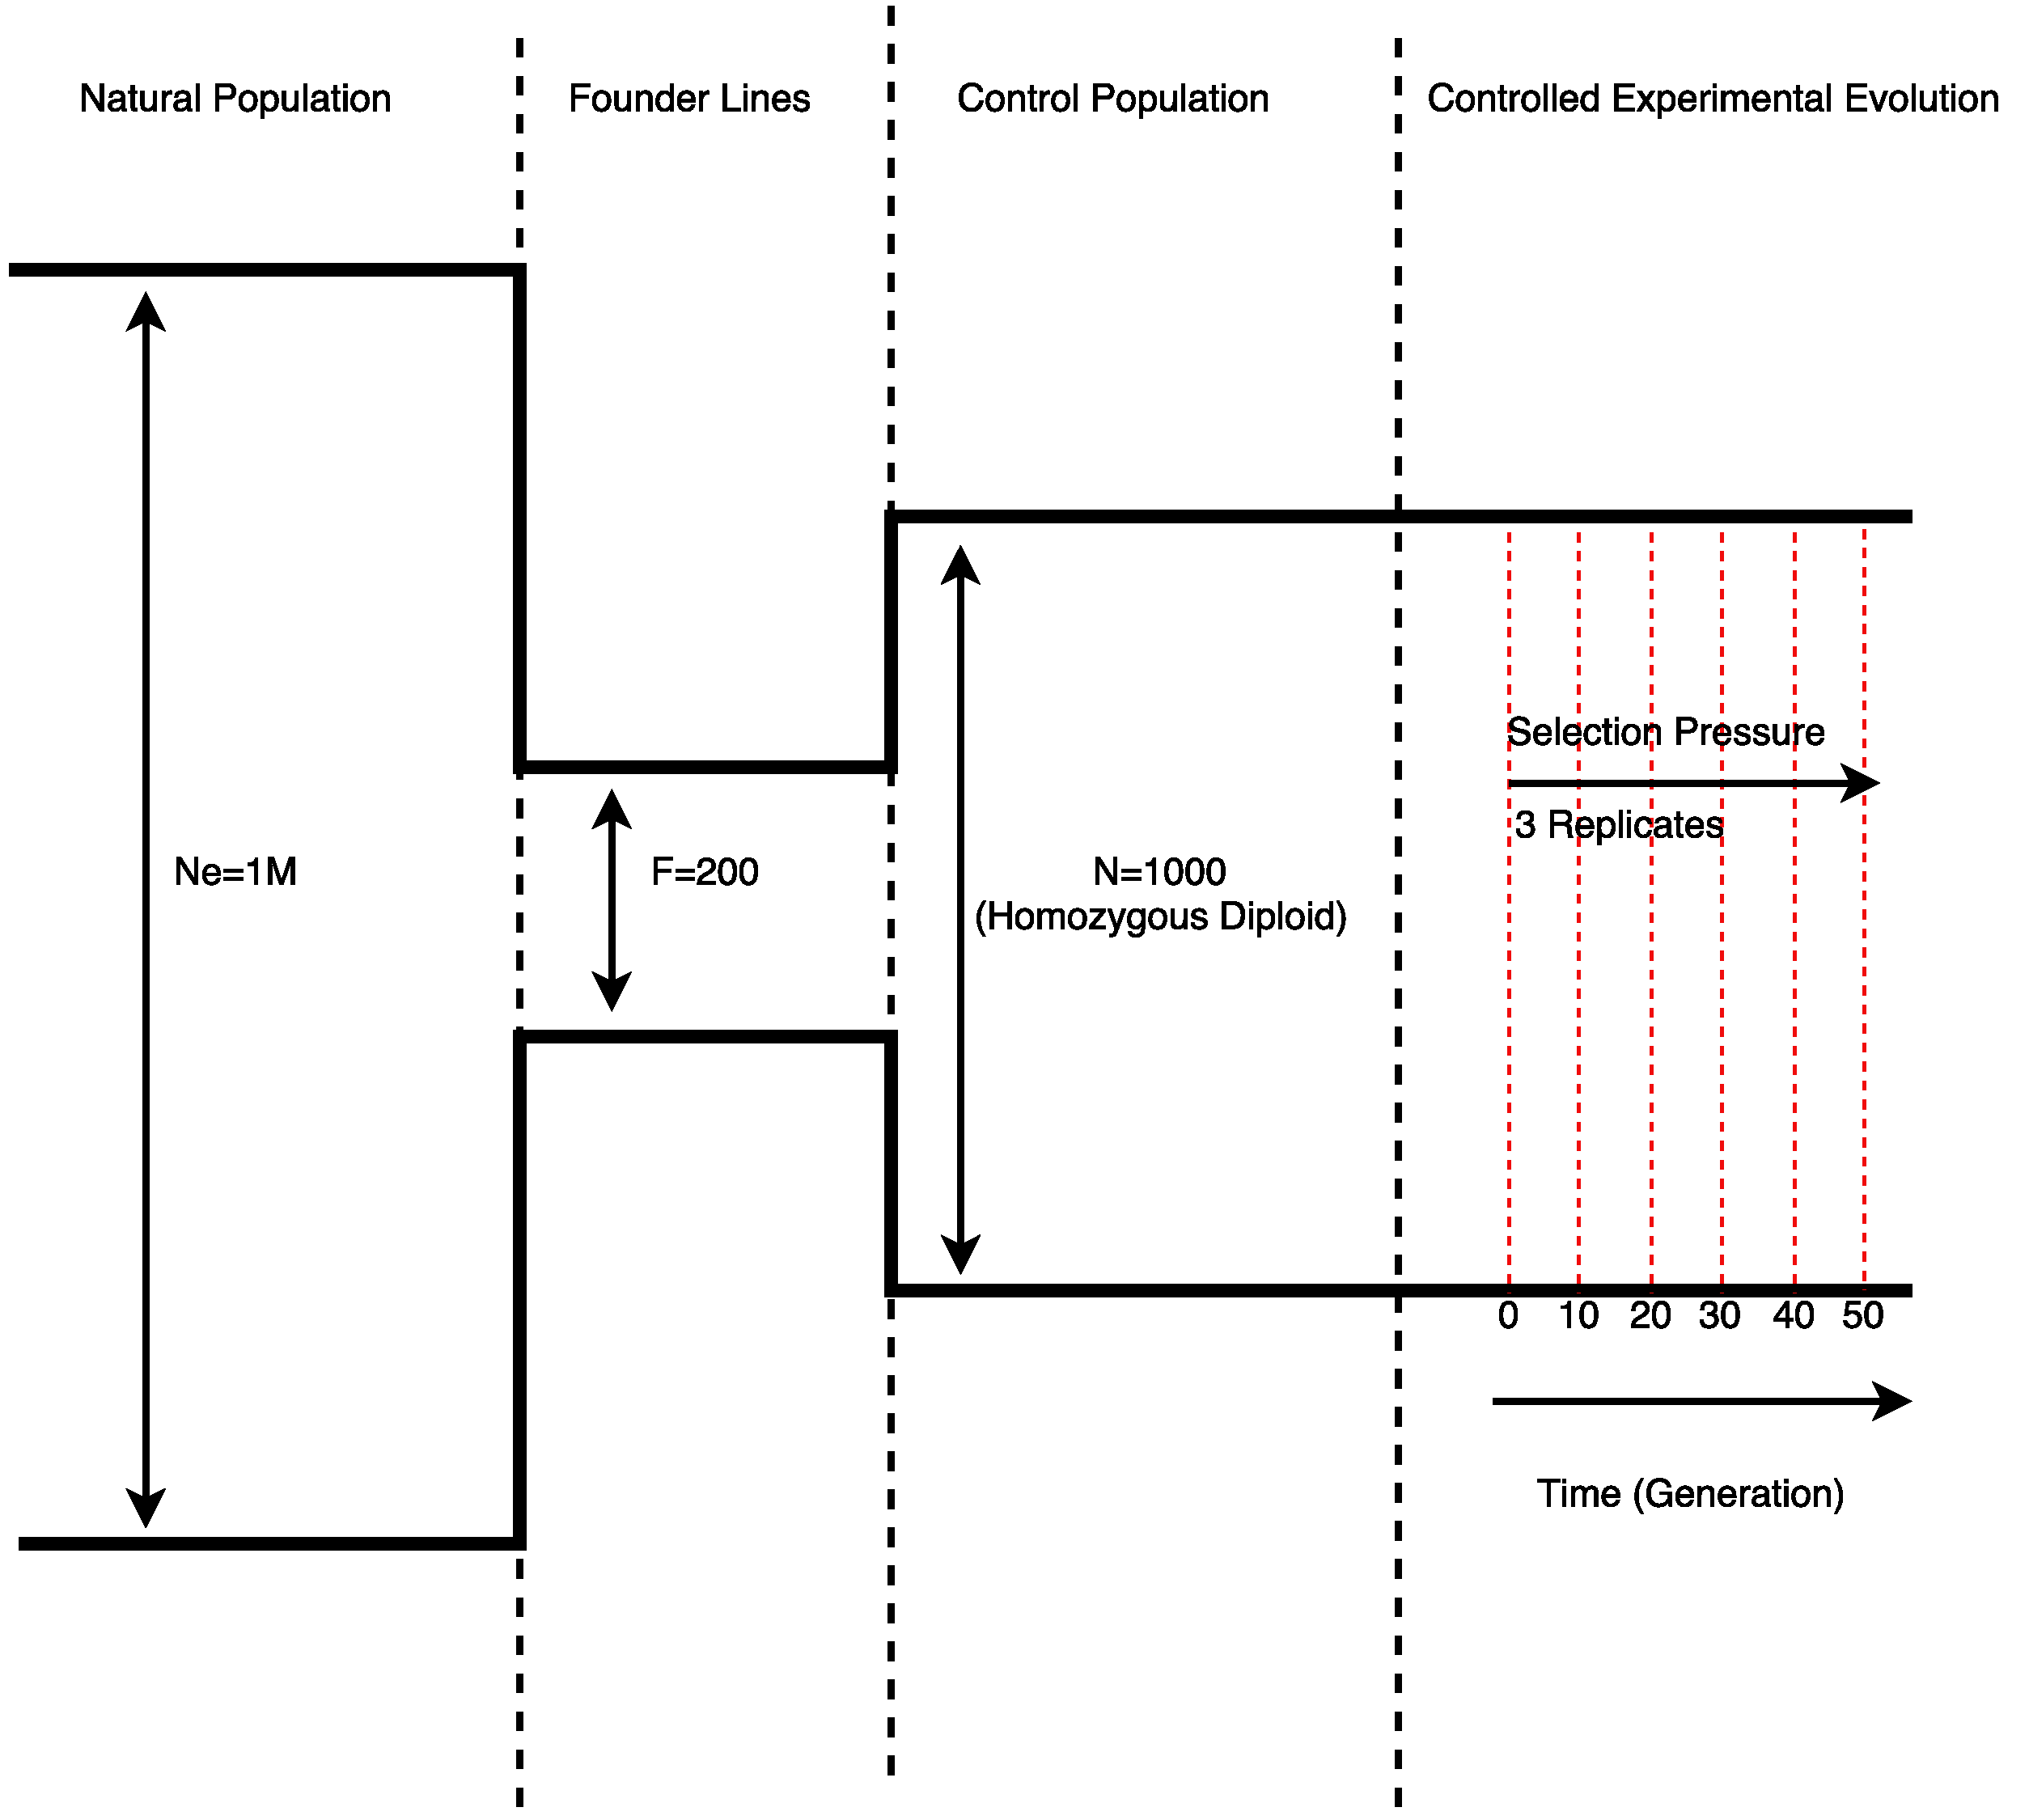
\includegraphics[trim=0.1in 0 .08in 0.02in , clip,width=0.5\textwidth]{figures/ControlledExperimentalEvolution.pdf}
&	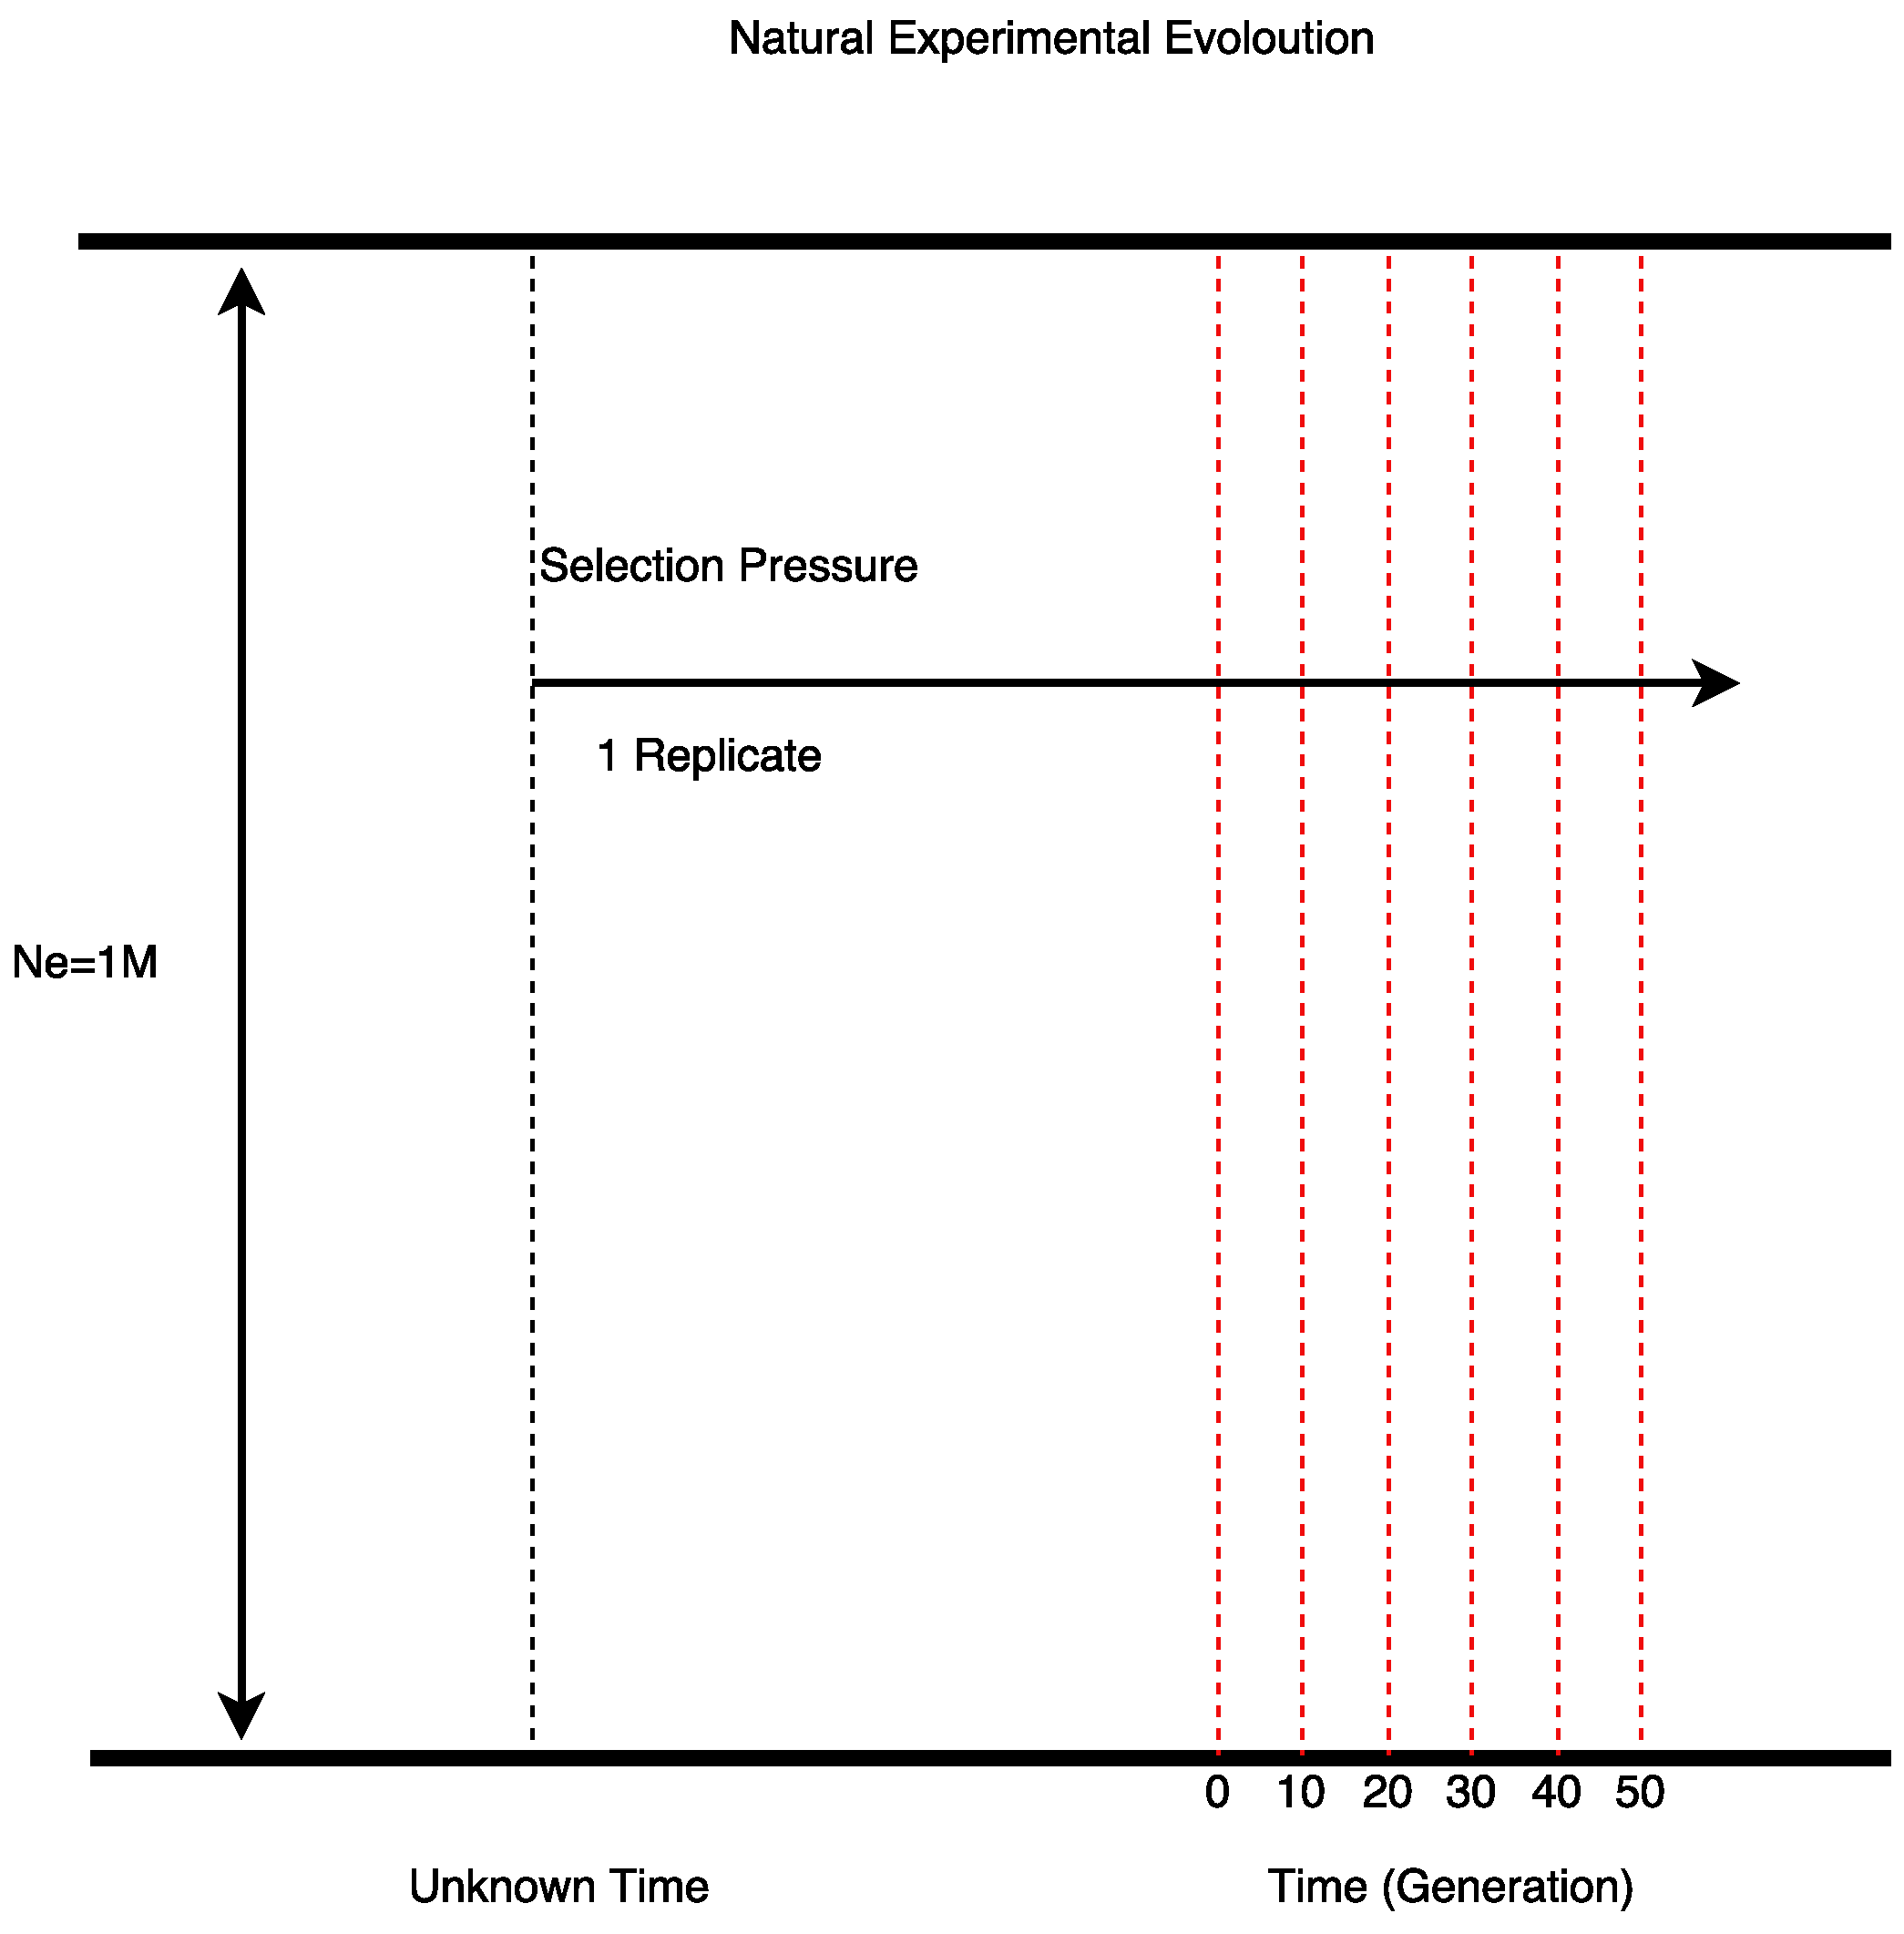
\includegraphics[trim=0.1in 0 .08in 0.02in , clip,width=0.5\textwidth]{figures/NaturalExperimentalEvolution.pdf}
	\end{tabular}
	\caption{ Simulations for Experimental Evolution and Natural
          evolution. } \label{fig:ee}
\end{figure}

\clearpage
\newpage

\begin{figure}[H]
	\centering
	\includegraphics[trim={1in 0.1in 0in 
		0in},clip,width=\textwidth]{figures/{markovDists}.pdf}


              \caption{{\bf Comparison of empirical distributions of
                  allele frequencies (green) versus predictions from
                  Brownian Motion (red), and Markov
                  Likelihoods}. Panels A-F: Experiments were conducted
                under neutral evolution with different starting
                frequencies $\nu_0\in\{0.005,0.1\}$ and sampling times
                $\tau \in \{1,10,100\}$ generations. The empirical
                distribution was computed by sampling 143,900 sites
                with $\nu_0=0.005$ and 47,500 with variants
                $\nu_0=0.1$.  computed from neutrally evolving
                simulations is depicted in green lines. Panels G,H,I:
                Comparisons of Empirical and Markov chain based
                predicted allele frequency value distributions under a
                selection regime with $s=0.1$. Initial frequency was
                chosen as $\nu_0=0.005$ and sampling performed after
                $t=\{1,10,100\}$ generations.}
	\label{fig:markov}
\end{figure}

\begin{figure}[H]
	\centering
	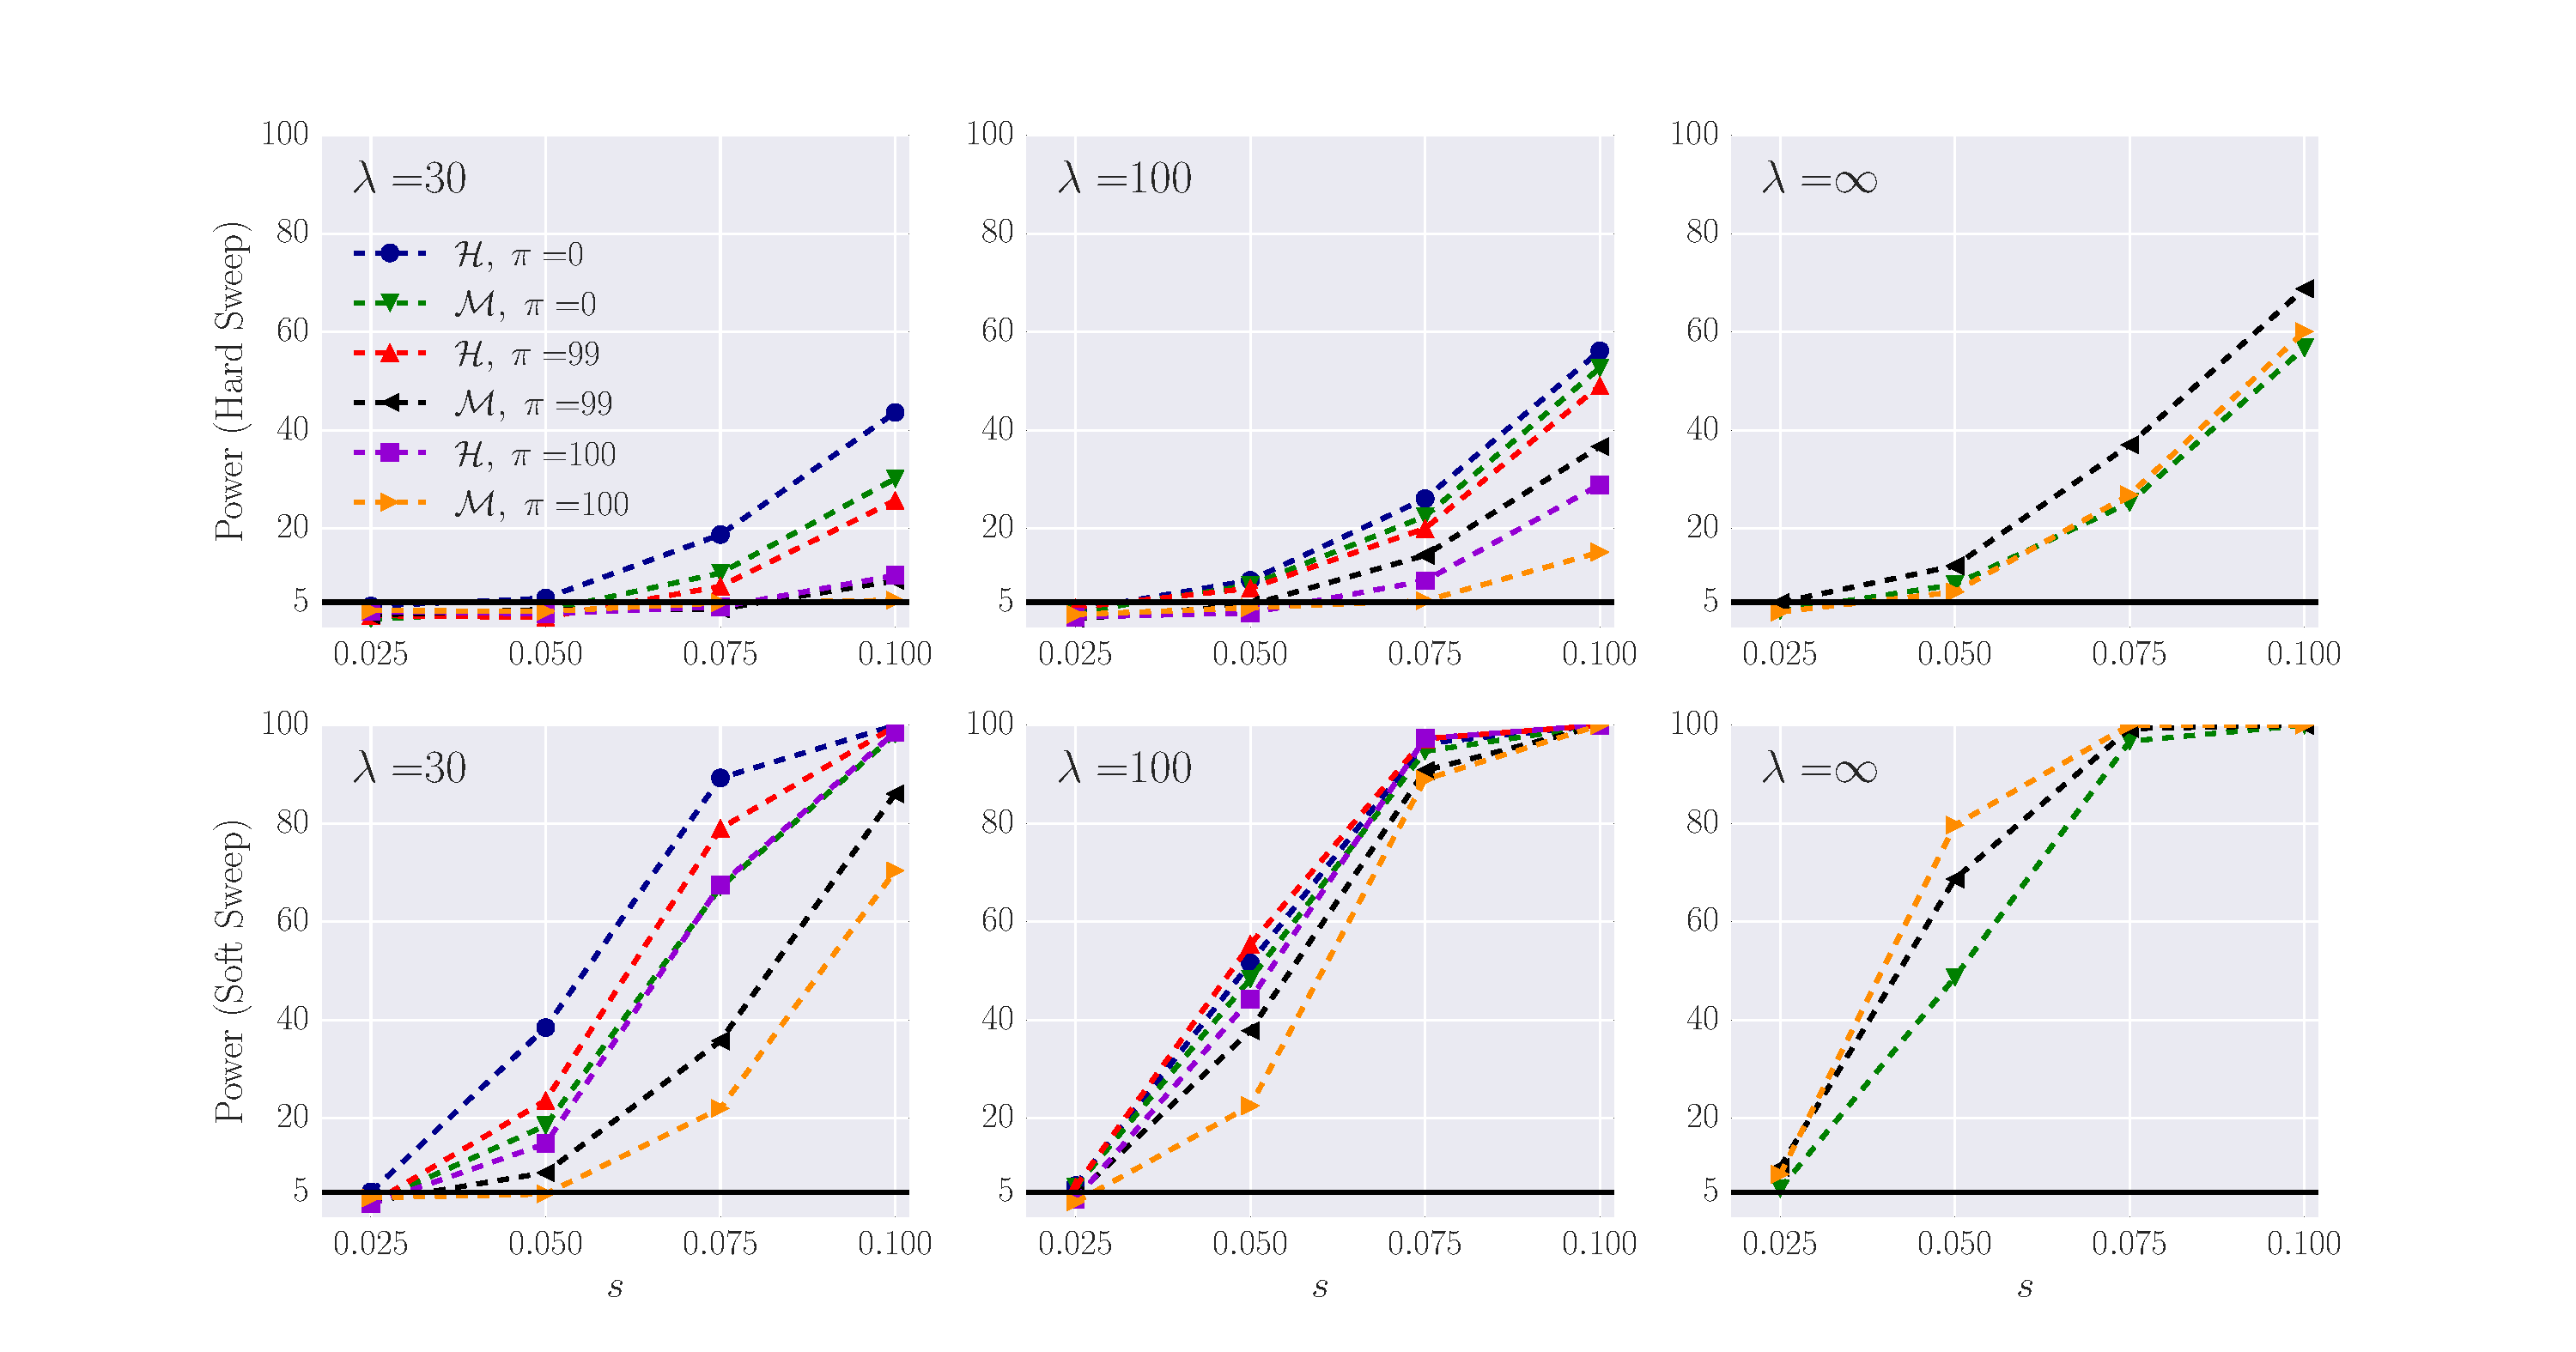
\includegraphics[trim=0.4in 0 .8in 0.02in , clip,width=\textwidth]{figures/powerCLR.pdf}
	\caption{{\bf Power calculations for detection of selection.} $1000$
          simulations were performed for each choice of selection
          coefficient $s$, and initial carrier frequency
          $\nu_0$. Power was computed as average true-positive-rate of
          detecting selection in a 50Kbp region, while
          FDR$\le$0.05.} \label{fig:powerCLR}
\end{figure}

\begin{figure}[H]
	\centering
	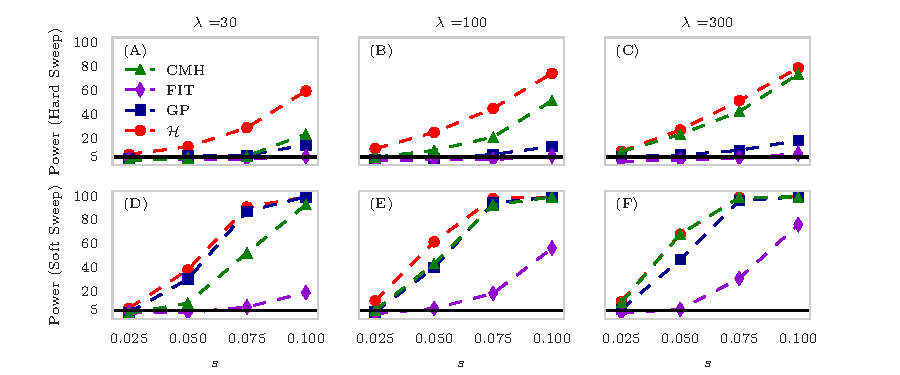
\includegraphics[trim=0.4in 0 .8in 0.02in , clip,width=\textwidth]{figures/power.pdf}
	\caption{ Power, average
          true-positive-rate when FDR$\le$0.05, for detecting
          selection in a 50Kbp region for Frequency Increment Test
          (FIT), Gaussian Process (GP), Markov Chain ($\Mc$), Hidden
          Markov Model ($\Hc$) on 1000 simulations for each of
          selection strength $s$ and initial carrier frequency
          $\nu_0$. To incorporate ascertainment bias, each setting is
          evaluated such that depth of each SNP is identically
          distributed from Poisson$(\lambda)$ for $\lambda \in
          \{30,100,\infty\}$. Average performance of each method is
          shown in Table \ref{tab:power}. Note that $\Hc$ and $\Mc$
          become identical when $\lambda=\infty$.  } \label{fig:power}
\end{figure}

\begin{figure}[H]
	\centering
	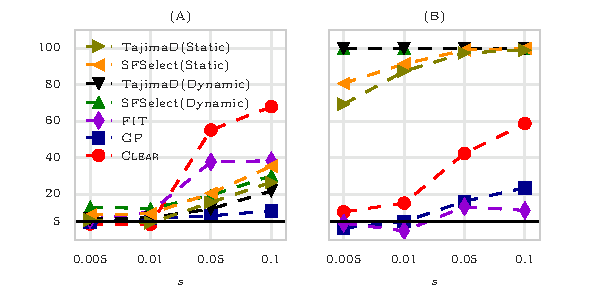
\includegraphics[trim=.4in 0 .8in 0.6in , clip,width=\textwidth]{figures/naturalee.pdf}
	\caption{{\bf power of SFS based statistics.} Power, average
          true-positive-rate when FDR$\le$0.05, for detecting
          selection in a 50Kbp region for Frequency Increment Test
          (FIT), Gaussian Process (GP), Markov Chain ($\Mc$)on 200
          simulations hard-sweep natural experimental evolution with
          $N_e=10^4$, for each of selection strength $s$. In this
          experiment start of sampling is random, then 5 samples are
          taken every 10 generations. (a) Start of sampling is chosen
          randomly throughout the sweep $\tau_1 \sim
          U\left[1,t_{\nu=1}(s,N_e)\right]$ (left) and chosen in the
          finale of the sweep $\tau_1 \sim
          U\left[t_{\nu=0.9}(s,N_e),t_{\nu=1}(s,N_e)\right]$ (right),
          where $t_{\nu=x}(s,N_e)$ to be understood as the number of
          expected generations required to reach carrier frequency $x$
          in a hard sweep and $U[a,b]$ is discrete uniform
          distribution.} \label{fig:powerSFS}
\end{figure}

\newpage
\begin{figure}[H]
	\centering
	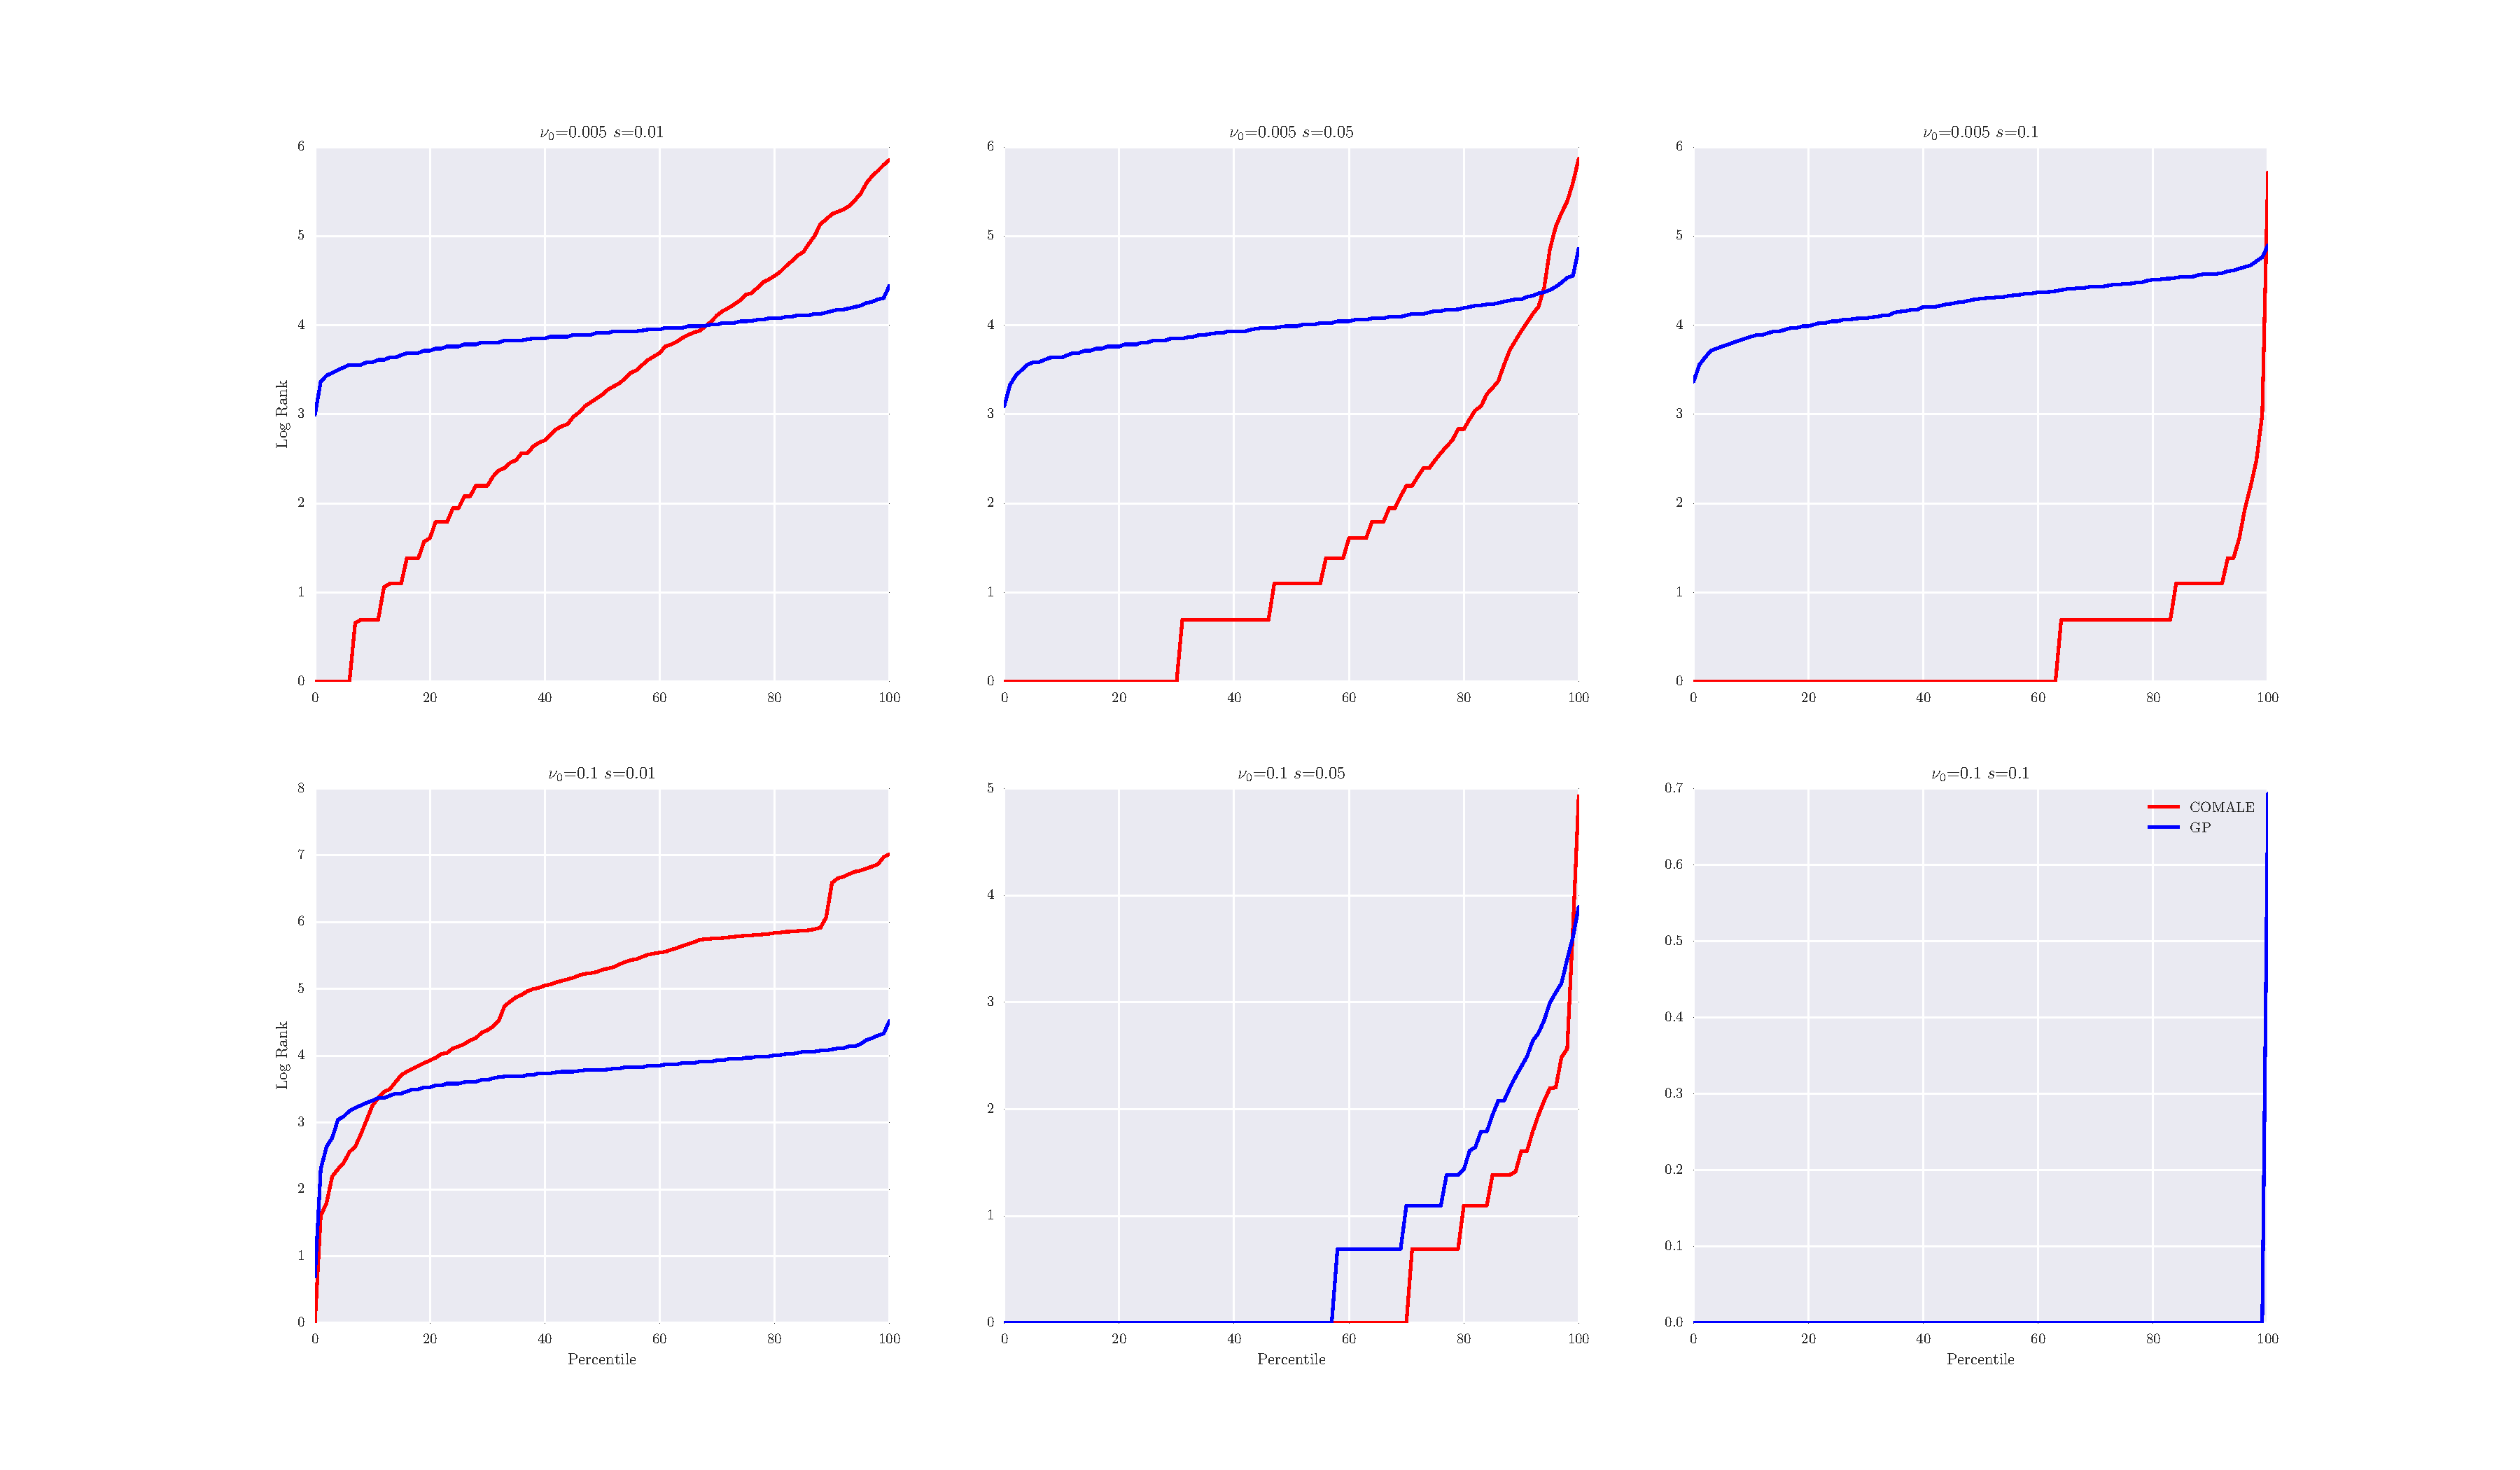
\includegraphics[trim=.2in 0 .2in 0, 
	clip,width=\textwidth]{figures/rank.pdf}
	\caption{Cumulative Distribution  Function (CDF) of the distribution of the rank of the adaptive allele in 500 simulations for Markov Chain ($\Mc$), Gaussian Process (GP) and Frequency Increment Test (FIT), for different values of selection strength $s$ and initial carrier frequency. Area Under Curve (AUC) is computed as a quantitative measure ranking performance of methods for each configuration.}
	\label{fig:rank}
\end{figure}

\begin{figure}[H]
	\centering
	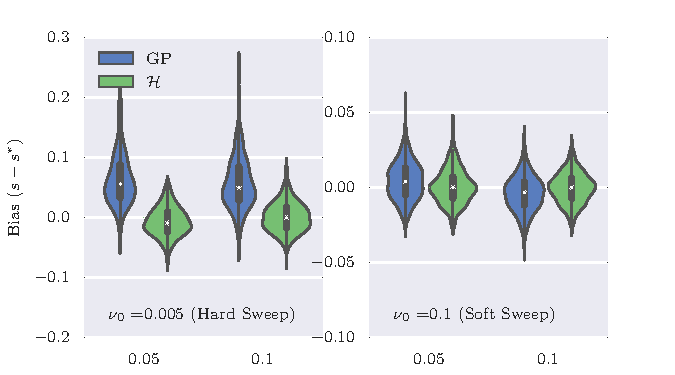
\includegraphics[trim=.0in 0 .2in 0 , clip,width=\textwidth]{figures/bias.pdf}
	\caption{Distribution of bias ($s-s^*$) over 500 simulations for each value of strength of selection $s$ and starting carrier frequency $\nu_0$.} \label{fig:bias}
\end{figure}
\begin{figure}[H]
	\centering
	\includegraphics[width=0.75\textwidth]{figures/{runTime.png}}
	\caption{Average running time of \comale, HMM, GP with single,3,5,7 and 10 loci over 1000 simulations. Average running time for each method is shown in the horizontal axis ticks.} 
	\label{fig:runTime}
\end{figure}

\begin{figure}[H]
	\centering
	\includegraphics[width=\textwidth]{figures/{manhattan.min500snp}.pdf}
	\caption{Manhattan plot of the composite $\Hc$ statistic (top) 
		and the number of SNPs (bottom) in 50Kbp sliding window with steps of 
		10Kbp, excluding windows with less that 500 SNPs. Regions in which 
		their $\Hc$ statistic falls in top one percentile 
		distribution is denoted with red color. Pearson correlation between $M$ 
		and 
		$\Hc$ of all windows is -0.09 and for the candidate regions is -0.08. 
		This indicates the spurious effect of windows with low diversity is 
		removed from out study (potentially at cost of some false negatives). } 
	\label{fig:manhattancutoffed}
\end{figure}



\clearpage
\newpage
\begin{table}[h]
	\begin{tabular}{c}
		\centering \begin{tabular}{c|p{4in}|c|c}
Rank	&GO Term	&-log($p$-value)	&Num of Genes\\\hline
1	&integral component of plasma membrane	&8.5	&264\\
2	&transcription factor activity, sequence-specific DNA binding	&5.6	&519\\
3	&central nervous system development	&5.5	&100\\
4	&plasma membrane	&5.4	&786\\
5	&dendrite morphogenesis	&5.4	&219\\
6	&L-ascorbic acid binding	&4.9	&24\\
7	&procollagen-proline 4-dioxygenase activity	&4.9	&26\\
8	&regulation of transcription, DNA-templated	&4.8	&398\\
9	&integral component of membrane	&4.5	&1434\\
10	&muscle organ development	&4.5	&75\\
11	&sequence-specific DNA binding	&4.3	&255\\
12	&oxidoreductase activity, acting on single donors with incorporation of molecular oxygen, incorporation of two atoms of oxygen	&4.3	&26\\
13	&protein kinase activity	&4.0	&179\\
\end{tabular}

	\end{tabular}
	\caption{GO enrichment when all the SNPs in the genes are taken into 
	account. .}\label{tab:transcriptGO}
\end{table}
\begin{table}[h]
	\begin{tabular}{c}
		\centering \begin{tabular}{c|p{4in}|c|c}
Rank	&GO Term	&-log($p$-value)	&Num of Genes\\\hline
1	&integral component of plasma membrane	&9.1	&264\\
2	&dendrite morphogenesis	&6.5	&219\\
3	&central nervous system development	&6.4	&100\\
4	&transcription factor activity, sequence-specific DNA binding	&6.4	&519\\
5	&plasma membrane	&6.1	&786\\
6	&regulation of transcription, DNA-templated	&5.4	&398\\
7	&integral component of membrane	&4.9	&1431\\
8	&ventral cord development	&4.7	&86\\
9	&protein kinase activity	&4.7	&179\\
10	&muscle organ development	&4.5	&75\\
11	&sequence-specific DNA binding	&4.4	&255\\
12	&L-ascorbic acid binding	&4.4	&24\\
13	&procollagen-proline 4-dioxygenase activity	&4.4	&26\\
14	&axon guidance	&4.3	&302\\
15	&mitochondrial translation	&4.3	&91\\
16	&neuropeptide signaling pathway	&4.1	&102\\
\end{tabular}

	\end{tabular}
	\caption{GO enrichment when synonymous variants are 
	excluded.}\label{tab:nonsynonymousGO}
\end{table}

\begin{table}[h]
	\begin{tabular}{c}
		\centering \begin{tabular}{c|c|p{4in}|c|c}
Rank	&GO ID	&GO Term	&-log($p$-value)	&Num of Genes\\\hline
1	&GO:0004656	&procollagen-proline 4-dioxygenase activity	&5.8	&26\\
2	&GO:0016702	&oxidoreductase activity, acting on single donors with incorporation of molecular oxygen, incorporation of two atoms of oxygen	&5.5	&26\\
3	&GO:0031418	&L-ascorbic acid binding	&4.9	&24\\
4	&GO:0005506	&iron ion binding	&4.5	&120\\
5	&GO:0016222	&procollagen-proline 4-dioxygenase complex	&4.2	&17\\
6	&GO:0048149	&behavioral response to ethanol	&4.0	&49\\
\end{tabular}

	\end{tabular}
	\caption{GO enrichment on missense variants.}\label{tab:exonGO}
\end{table}
\begin{table}[h]
	\begin{tabular}{c}
		\centering \begin{tabular}{c|c|p{4in}|c|c}
Rank	&GO ID	&GO Term	&-log($p$-value)	&Num of Genes\\\hline
1	&GO:0005886	&plasma membrane	&3.0	&34\\
\end{tabular}

	\end{tabular}
	\caption{GO enrichment on loss of function variants.}\label{tab:lofGO}
\end{table}


\begin{table}[h]
	\begin{tabular}{c}
		\centering \begin{tabular}{c|c|p{3in}|c|c|c}
Rank	&GO ID	&GO Term	&-log($p$-value)	&Hits	&Num of Genes\\\hline
1	&GO:0004046	&aminoacylase activity	&9.7	&5	&7\\
2	&GO:0006520	&cellular amino acid metabolic process	&6.4	&5	&18\\
3	&GO:0015101	&organic cation transmembrane transporter activity	&6.4	&3	&5\\
4	&GO:0007501	&mesodermal cell fate specification	&6.2	&4	&11\\
5	&GO:0004601	&peroxidase activity	&5.1	&4	&17\\
6	&GO:0006979	&response to oxidative stress	&5.0	&8	&79\\
7	&GO:0007483	&genital disc morphogenesis	&4.7	&2	&4\\
8	&GO:0045664	&regulation of neuron differentiation	&4.7	&2	&4\\
9	&GO:0045787	&positive regulation of cell cycle	&4.3	&2	&5\\
10	&GO:0008074	&guanylate cyclase complex, soluble	&4.3	&2	&5\\
11	&GO:0009312	&oligosaccharide biosynthetic process	&4.2	&3	&13\\
12	&GO:0004653	&polypeptide N-acetylgalactosaminyltransferase activity	&4.1	&3	&14\\
13	&GO:0070864	&sperm individualization complex	&4.0	&2	&6\\
14	&GO:0008324	&cation transmembrane transporter activity	&4.0	&2	&6\\
15	&GO:0008599	&protein phosphatase type 1 regulator activity	&4.0	&2	&6\\
16	&GO:0008378	&galactosyltransferase activity	&3.8	&2	&7\\
17	&GO:0007492	&endoderm development	&3.8	&2	&7\\
18	&GO:0000302	&response to reactive oxygen species	&3.8	&2	&7\\
19	&GO:0040014	&regulation of multicellular organism growth	&3.6	&3	&18\\
20	&GO:0016485	&protein processing	&3.5	&3	&19\\
21	&GO:0006030	&chitin metabolic process	&3.5	&7	&99\\
22	&GO:0020037	&heme binding	&3.4	&8	&127\\
23	&GO:0005815	&microtubule organizing center	&3.4	&2	&9\\
24	&GO:0042659	&regulation of cell fate specification	&3.4	&2	&9\\
25	&GO:0007415	&defasciculation of motor neuron axon	&3.4	&2	&9\\
26	&GO:0045297	&post-mating behavior	&3.2	&2	&10\\
27	&GO:0010212	&response to ionizing radiation	&3.2	&2	&10\\
28	&GO:0007519	&skeletal muscle tissue development	&3.2	&2	&10\\
29	&GO:0051865	&protein autoubiquitination	&3.2	&2	&10\\
30	&GO:0006182	&cGMP biosynthetic process	&3.2	&2	&10\\
31	&GO:2000134	&negative regulation of G1/S transition of mitotic cell cycle	&3.1	&2	&11\\
32	&GO:0044212	&transcription regulatory region DNA binding	&3.1	&2	&11\\
33	&GO:0040015	&negative regulation of multicellular organism growth	&3.1	&2	&11\\
34	&GO:0036011	&imaginal disc-derived leg segmentation	&3.1	&2	&11\\
35	&GO:0008061	&chitin binding	&3.1	&7	&113\\
36	&GO:0004702	&receptor signaling protein serine/threonine kinase activity	&3.0	&3	&26\\
\end{tabular}

	\end{tabular}
	\caption{Gene set enrichment of 243 genes within 25 intervals under 
	selection using Fisher exact test.}\label{tab:Fisher}
\end{table}

\newpage


%\section{Introduction}

Genetic adaptation is \emph{the} central evolutionary process and is
at the core of some of the greatest challenges facing humanity. HIV
would likely cause nothing more than harmless fever without the
ability of the virus to adapt and eventually destroy the immune
system. Cancer would be much more straightforward to treat if not for
tumor's ability to adapt to anti-cancer drugs. Malaria could be
treated with cheap drugs such as quinine instead of being one of the
world's worst killers. Crop pests would be manageable with small doses
of safe insecticides instead of requiring applications of ever
increasing amounts of a diverse array of powerful chemicals. In both
disease and agriculture, we find ourselves in an arms race due to the
ability of organisms to adapt.

Adaptation leaves a variety of detectable signatures in
genomes~\cite{Akey09, Kreitman00, MesserAndPetrov13, Nielsen05,
  SabetiEtAl06}. The rapid expansion of adaptive alleles in
populations leads to both an excess of functional changes between
species and distortions in polymorphism patterns known as selective
sweeps~\cite{Nielsen05}. The signatures of selective sweeps, which
include reduction of levels of polymorphism and the presence of too
many rare alleles~\cite{Nielsen05, Przeworski02}, have been the basis
for assessing genomic patterns in many genome scans for
adaptation. Classical tests such as the well-known Tajima's \emph{D}
statistic~\cite{Tajima89} that rely on the \emph{site-frequency
  spectrum}---a list of counts of the numbers of genomic sites in a
region with each of the different possible allele frequencies---have
been among the first steps in genomic detection of selection, but they
have largely been chosen in a non-systematic manner to identify quite
specific rather than general signatures of selection, and they have
often faced the problem of confounding of positive selection with
demographic processes~\cite{PtakAndPrzeworski02, RamosOnsinsAndRojas}.
Part of the challenge is that studies on natural populations are
conducted on a extant populations, a single window in a complex,
uncontrolled process.

Experimental evolution (including evolve and re-sequence paradigms)
have become increasingly popular as a complementary tool to understand
the forces of selection, allowing for controlled environments,
specific selection constraints. Examples of experimental evolution
studies abound in sexual populations, particularly in fruitfly. Burke
et al.~\cite{Burke2010} evolved flies for over $600$ generations under
selection for accelerated development, and noted that evolution for
sexual populations is very different from those of asexual populations
(e.g., Lenski~\cite{}): the effects of clonal interference is slower
due to recombination that allows for the incorporation of multiple
beneficial alleles, but there are fewer, unconditionally advantageous
alleles that arise at the onset of selection. Rose and
Colleagues~\cite{Rose} created $200$ experimentally evolved
populations selected for different traits, starting with $10$ initial
populations. Zhou et al. evolved flies to adapt to low oxygen
environment (hypoxia) for over $300$ generations, and identified many
genes involved in hypoxia tolerance~\cite{}.  Instead, they observed
incomplete fixation (`soft-sweeps') due in part to standing variation,
changing selection coefficients, and small fitness effects.

Much like in natural populations, many of these studies also
sequenced/genotyped only the latest population. However, the emergence
of NGS and related technologies has made it feasible to sequence the
evolving population at multiple time points in its evolution. At the
same time, for small organisms where a single animal does not provide
enough DNA, it is more effective to pool together individuals in the
population at a particular time point, in a single sequencing
experiment. Thus, instead of individual genotypes, we obtain
frequencies of the derived allele at all loci at different time
points. Methods for analyzing such time series pooled sequence data
are only just being developed.

In this paper we aim to use the tools and machinery that has been
developed for RNNs, to model times-series biological data. In
particular, we consider the population genetics problem of finding
loci (locus) under selection given observation of allele frequency of
a population in different generations of a Wright-Fisher model. This
problem has been previously treated by using Gaussian Processes
\cite{EnadR-GP}, spectral methods \cite{EandR-spectral}




%\section{Methods}
In this section we formally present describe RNN model and a Naive method which takes $\Oc(1)$ computations as baseline performance.

\subsection{Notation}
In this paper, we denote Tensor with bold-faced capital letter, matrices with capital letter, vectors with bold-faced small letter, and scalars with small letters. Let $\bfX \in [0,1]^{R \times T \times L}$  be the Tensor of containing allele frequencies of the population where $R,L,T$ are number of experimental replicates, samples in time, segregating sites, respectively. Also, in our simplified notation $X_r=[\bfx_1 ,\cdots, \bfx_L]\in  [0,1]^ {T \times L}$  data matrix for replicate $r$,  $\bfx_l =[x_1,\cdots,x_T]$ is the observation at locus $i$ for a given replicate, and $x_t\in [0,1]$ is the allele frequency at time $t$ for a given replicate and locus. It should be noted that $T=|\Tc|$ where $\Tc=\{\tau_1,\tau_2,\cdot, \tau_T \}$ is the set of times (generations) of samples which pool sequencing data is collected. For examples $\Tc=\{2,18,25\}$ denotes that the dataset contains allele frequency of the population at 2nd, 18th and 25th generations.



\subsection{Regularized Nonlinear Least Squares}
For simplicity, in this paper we consider bi-allelic single-locus Wright-Fisher (WF) model with no mutations \cite{book-mathpopgen} which assumes  discrete generation, random mating etc. Under finite population size\footnote{In infinite population size we have $x_{t+1} = f(x_t;s,h)$.} assumption allele frequency at each generation is a random variable
\beq\label{eq:trans0}
x_{t+1} = f(x_t;s,h)  + \epsilon_t
\eeq
where $h$ is the overdominance, $\epsilon_t$ is random noise due to genetic drift at generation $t$ and $f: [0,1] \mapsto [0,1]$ is the transition function:
\beq
f(x)=\frac{(1+s)x^2 + (1+hs)x(1-x)}{(1+s)x^2 + 2(1+hs)x(1-x) + x(1-x)}=x+\frac{s(h+(1-2h)x)x(1-x)}{1+sx(2h+(1-2h)x))}
\eeq
Since the transition function depend on both $s$ and $h$, we can estimate both of them at the same time by solving a 2-dimensional optimization problem. However, for the sake of simplicity of notation we aim to only estimate $s$ and set $h=0.5$ 
\beq
f(x)=x+\frac{sx(1-x)}{2+2sx}
\eeq
Given $x_t$, we can consider \ref{eq:trans0} as a nonlinear function of $s$ and finding $s$ can be formulated as a classical a 1-dimensional non-linear least-squares problem \cite{•}
\beq \label{eq:nlls0}
s^*=\underset{s}{\arg \min} \| x_{t+1} -f(x_t;s,h)\|^2
\eeq
which can be solved by iterative optimization algorithms. 
However, \eqref{eq:nlls0} does not account for dependence of $x_t,x_{t-1}, \cdots$ to $s$. To incorporate this dependence, we introduce the notation
\beq
y_t(s)= \underbrace{f(\cdots f(}_tx_0;s))
\eeq
and we can find $s$ by solving
\beq
s^*=\underset{s}{\arg \min} \sum_{t=1}^T \| y_{\tau_t}(s)- x_{t} \|^2
\eeq
On the other hand, using ordinary differential equations (ODE), \eqref{eq:trans0} can be written as \cite{multilocus-hitchhike}:

\beq
y_t(s)=\frac{x_0}{x_0 +(1-x_0)e^{-s\tau_t/2}}= \frac{1}{1+ce^{-s\tau_t/2}} = \sigma(-s\tau_t/2)
\eeq
where $c=(1-x_0)/x_0$ is constant and $\sigma(.)$ is modified sigmoid function (due to presence of $c$). Therefore, we have
\beq
s^*=\underset{s}{\arg \min} \sum_{t=1}^T \frac{1}{2} \| \sigma(s\tau_t/2)- x_{t} \|^2 + \frac{\lambda }{2}s^2
\eeq
which is a standard 1-d nonlinear regularized nonlinear least squares (RNLLS) optimization problem. To solve it we need to use iterative optimization algorithms which require computing gradient\footnote{$\sigma'(s)=\sigma(s)(1-\sigma(s))$} w.r.t. $s$
\beq
g= \sum_{t=1}^T \frac{\tau_t}{2} ( \sigma(s\tau_t/2)- x_{t} ) \sigma(s\tau_t/2) (1-\sigma(s\tau_t/2)) + \lambda s
\eeq
By taking into account of all replicates, the gradient descent update is
\beq
s\leftarrow s - \eta \sum_{r=1}^R g_i
\eeq
where $\eta$ is learning rate. Also, since this problem is not convex, we use Nestrov's Accelerated Gradient (NAG) descent algorithm which which has shown to be successful on many nonconvex problems. Also it should be noted that each iteration of the optimization takes $\Oc(TR)$ computation which make the algorithm tractable.

\subsection{Gaussian Process}
The Gaussian Process optimizes
\beq
\underset{\theta}{ \arg \max} \ \ \Lc(\bfX | \theta)
\eeq
where $\Lc$ is Gaussian distribution log-likelihood, i.e. negative weighted least-squares loss. Mean and covariance functions of the GP at any $t,l$ are functionally dependent to parameter of interest $\theta$, and computed using transition function of the WF process \cite{EandR-GP}.

\subsection{Naive Method}
To have a baseline performance,  in this subsection we consider a scenario with infinite population size, i.e., 
\beq
x_t(s)=\frac{x_0}{x_0 +(1-x_0)e^{-s\tau_t/2}}
\eeq
Since $s$ assumed to be constant, we can solve for $s$
\beq
s_t=\frac{2}{\tau_t} \log \left( \frac{x_t (1-x_0)}{x_0 (1-x_t)} \right)
\eeq
and finally to reduce the variance we can average all the naive estimates:
\beq
s_{Naive}=\sum_{t=1}^T\frac{2}{\tau_t} \log \left( \frac{x_t (1-x_0)}{x_0 (1-x_t)} \right)
\eeq

%\section{Methods (Arya)}
\beq
  \frac{d\nu_t(s)}{dt} &=\frac{s}{2}\nu_t(s)(1-\nu_t(s))\frac{1}{1+s\nu_t(s)} \\
  \frac{st}{2}-c&=\log\left(\frac{\nu_0}{(1-\nu_0)^{1+s}}\right)
  
\eeq
\section{Experiments}
In this part we compare MLE with GP and Naive method. 
\subsection{Data}
\subsubsection{Simulations}
For each experiment a diploid population is created and evolved as follows. 
\paragraph{I. Creating initial founder lines}
First using msms prgram, we created a population for $F$ founding haplotypes with parameters \texttt{\$./msms <F> 1 -t <4μLNe> -r <4Ne(L − 1)r> <L>} where $F=200$ is number of founder lines, 
$L=10^5$, $\theta=4\mu LNe=17$ and $\rho=4Ne(L-1)r=4$.  (assuming $Ne=1000$, $r=10^{-8}$ and $\mu=4.25\times 10^{-8}$).  
\paragraph{II. Creating initial diploid population} 
To mimic the real E\&R experiment for diploid organisms, first initial haplotypes cloned to create $F$ diploid homozygotes. Then each diploid is cloned $N/F$ times to yield $N$ diploid homozygote organisms.
\paragraph{III. Forward Simulation}
Given initial diploid population, position of the site under selection, selection strength $s$, number of replicates $R=3$, recombination rate $r=10^{-8}$ and sampling times $\Tc=\{10,20,30,40,50\}$ simuPop is used to perform forward simulation and compute allele frequencies for all of the $R$.

\subsubsection{Real}

\subsection{Likelihood Ratio Test}
Using the MLE (and other) estimates of $s$ it is desirable to perform a secondary task such as \emph{testing for selection} or \emph{locating the site under selection}. Likelihood ratio test (LRT) statistics for time series \cite{feder2014} have shown to be predictors for differentiating neutral and natural selection evolution cases. For a single locus model, the likelihood ratio test statistics $\Lambda(s*)$ is defined
\beq \label{eq:lrt}
\Lambda(s^*) = \log \left(\frac{\Lc(\bfX|s=s*)}{\Lc(\bfX|s=0)}\right)
\eeq
where $s^*$ is the optimal solution for the maximum-likelihood procedure. For the Gaussian process and Gaussian model the likelihood $\Lc_{GP}$ and $\Lc_G$ are well defined and \eqref{eq:lrt} can be easily evaluated. The likelihood of the Naive method for estimating based on $x_t$ is 
\beq
\Lc_N(s|x_t,x_0)=x_t-\sigma(st/2 -c)
\eeq

In addition to LRT, the value of $s^*$ itself can be regarded as a signal for detecting selection. In other words, modifying the LRT to
\beq
\Theta=s^*\Lambda(s^*)
\eeq
will take into account of two different objectives, 1)model discrepancy from neutral model 2)strength of selection under non-neutral model. In the  results we show that the modified-LRT makes more accurate predictions.

\subsection{Results}
In this part we compare the computational and predictive performance of the proposed method in detecting selection, locating selection in the genome, and estimating strength of selection with Gaussian process and the outlined naive method.

\subsubsection{Detecting Selection}
Detecting selection in the whole genome is a non-trivial task in real world and can be regarded as a application for the proposed algorithm. To provide a fair and unbiased comparison, we computed the test statistic for 1000 simulations and computed Receiver Operative Characteristic curve and Area Under Curve (AUC) for each method.



\begin{figure}[H]
  \centering
    \includegraphics[width=\textwidth]{{roc0.01A0.01}.png}
  \caption{Rank}
  \label{fig:Fig3a}
\end{figure}

\begin{figure}[H]
  \centering
    \includegraphics[width=\textwidth]{{roc0.02A0.01}.png}
  \caption{Rank}
  \label{fig:Fig3b}
\end{figure}

\begin{figure}[H]
  \centering
    \includegraphics[width=\textwidth]{{roc0.05A0.01}.png}
  \caption{Rank}
  \label{fig:Fig3c}
\end{figure}

\begin{figure}[H]
  \centering
    \includegraphics[width=\textwidth]{{roc0.1A0.1}.png}
  \caption{Rank}
  \label{fig:Fig3d}
\end{figure}

\begin{table}
\centering
\begin{tabular}{ l |c c c c }
$s$& 0.01 &0.02 & 0.05 & 0.1 \\
\hline
  Gaussian Model & 2 & 3& 2 & 3 \\
Gaussian Process & 5 & 6 & 2 & 3\\
  Naive & 8 & 9 & 2 & 3\\
\end{tabular}
\caption{AUC of all method evaluated for 1000 simulations and different values of $s$.}
\end{table}


\subsubsection{Finding Site Under Selection}
\paragraph{Distance}
\begin{figure}[H]
  \centering
    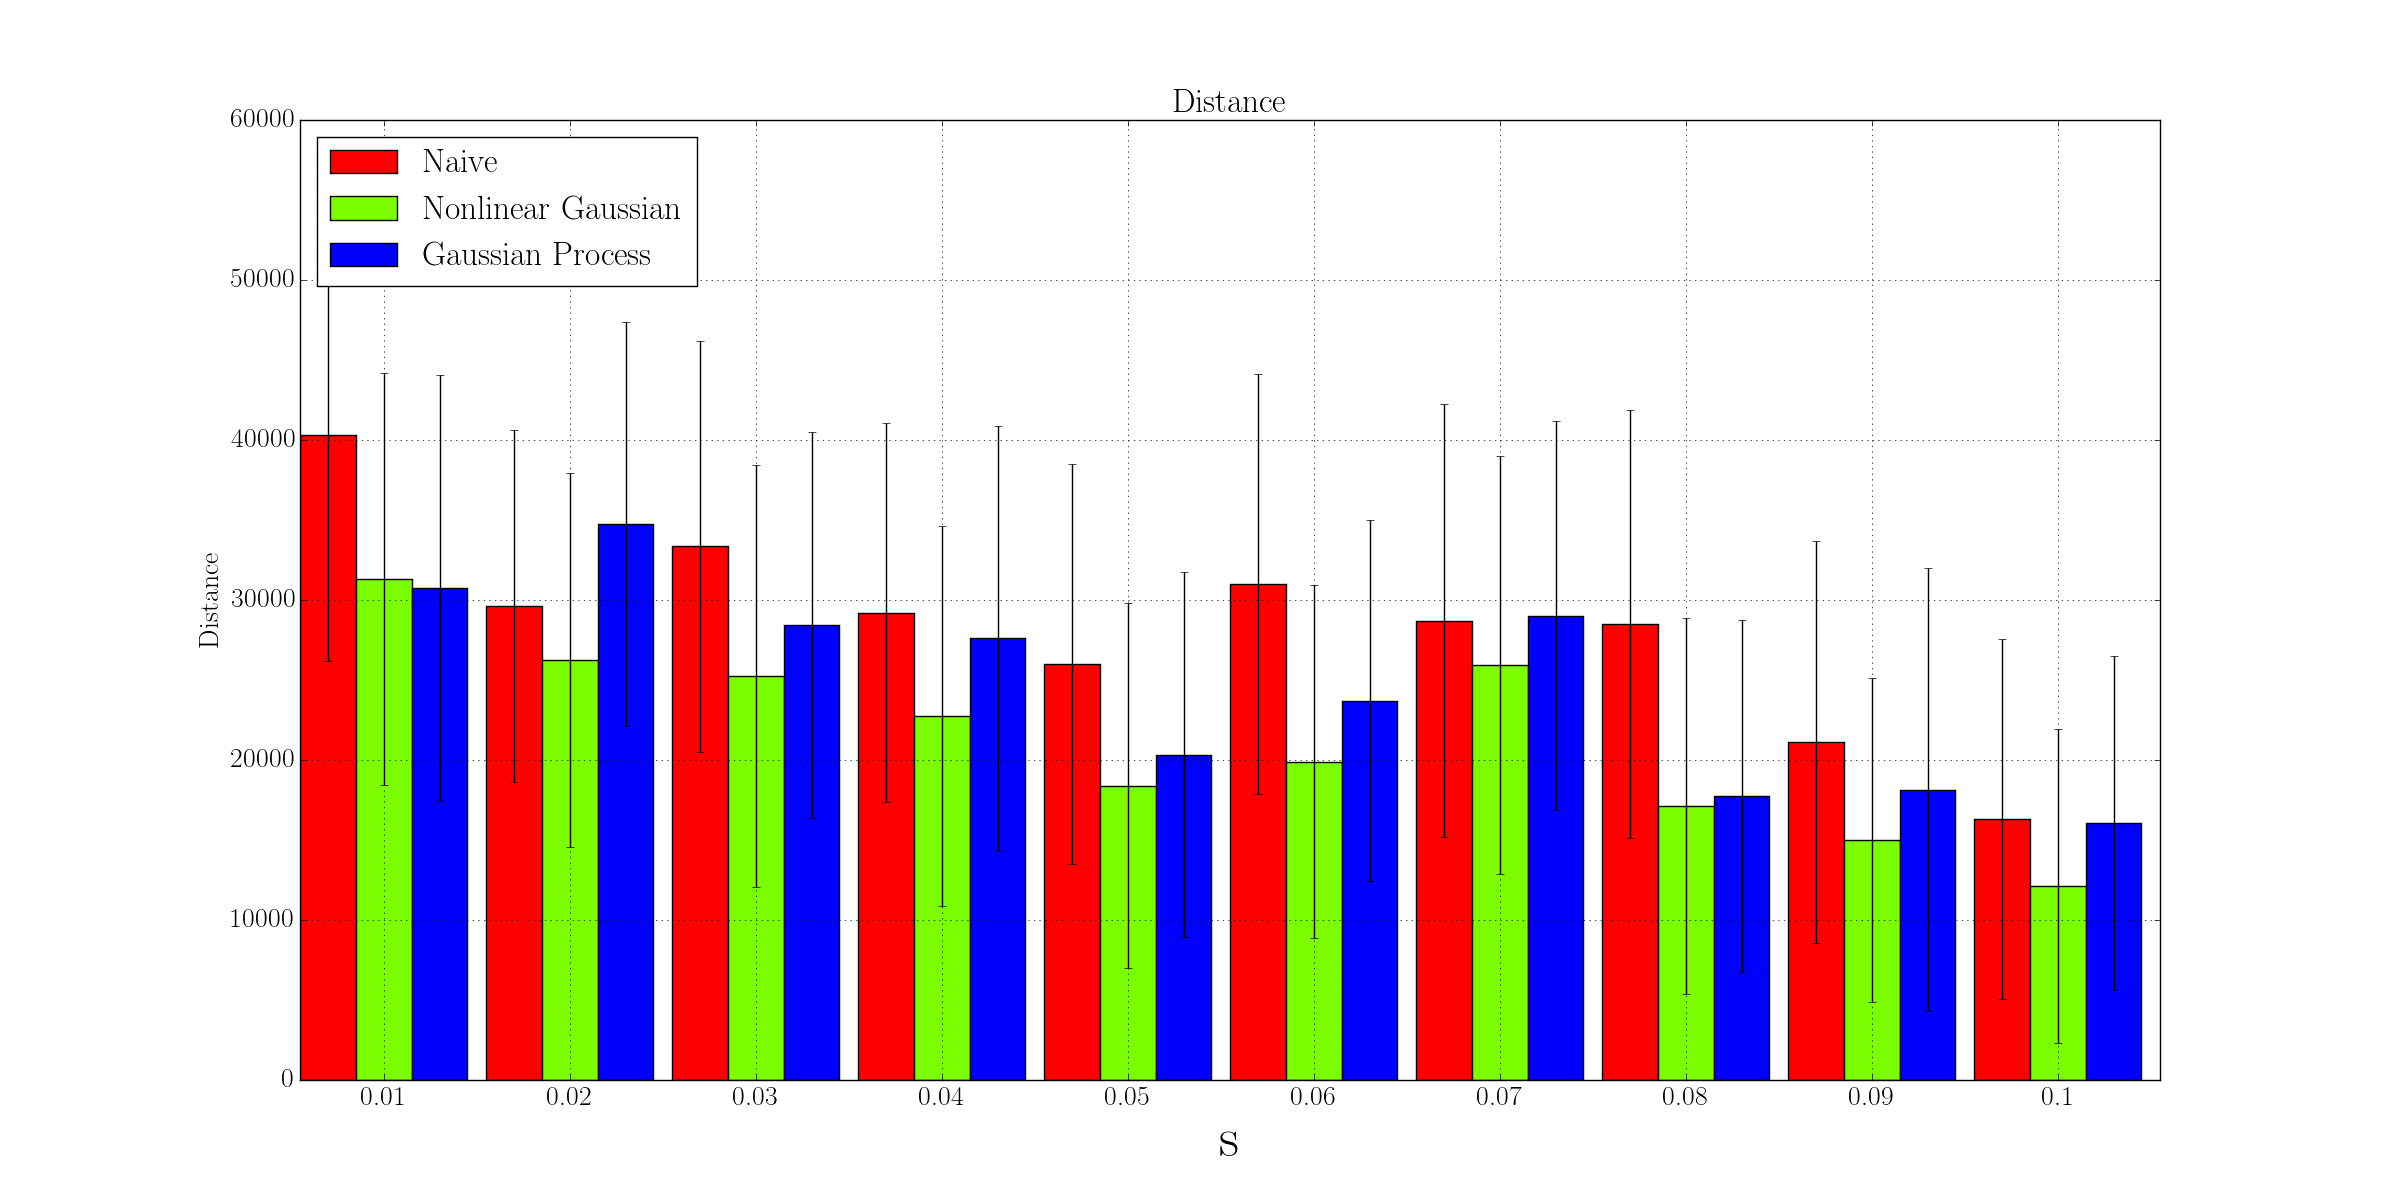
\includegraphics[width=\textwidth]{dist}
  \caption{Average distance to predicted site to the true site that is under selection.}
  \label{fig:Fig1}
\end{figure}

\paragraph{Rank}
\begin{figure}[H]
  \centering
    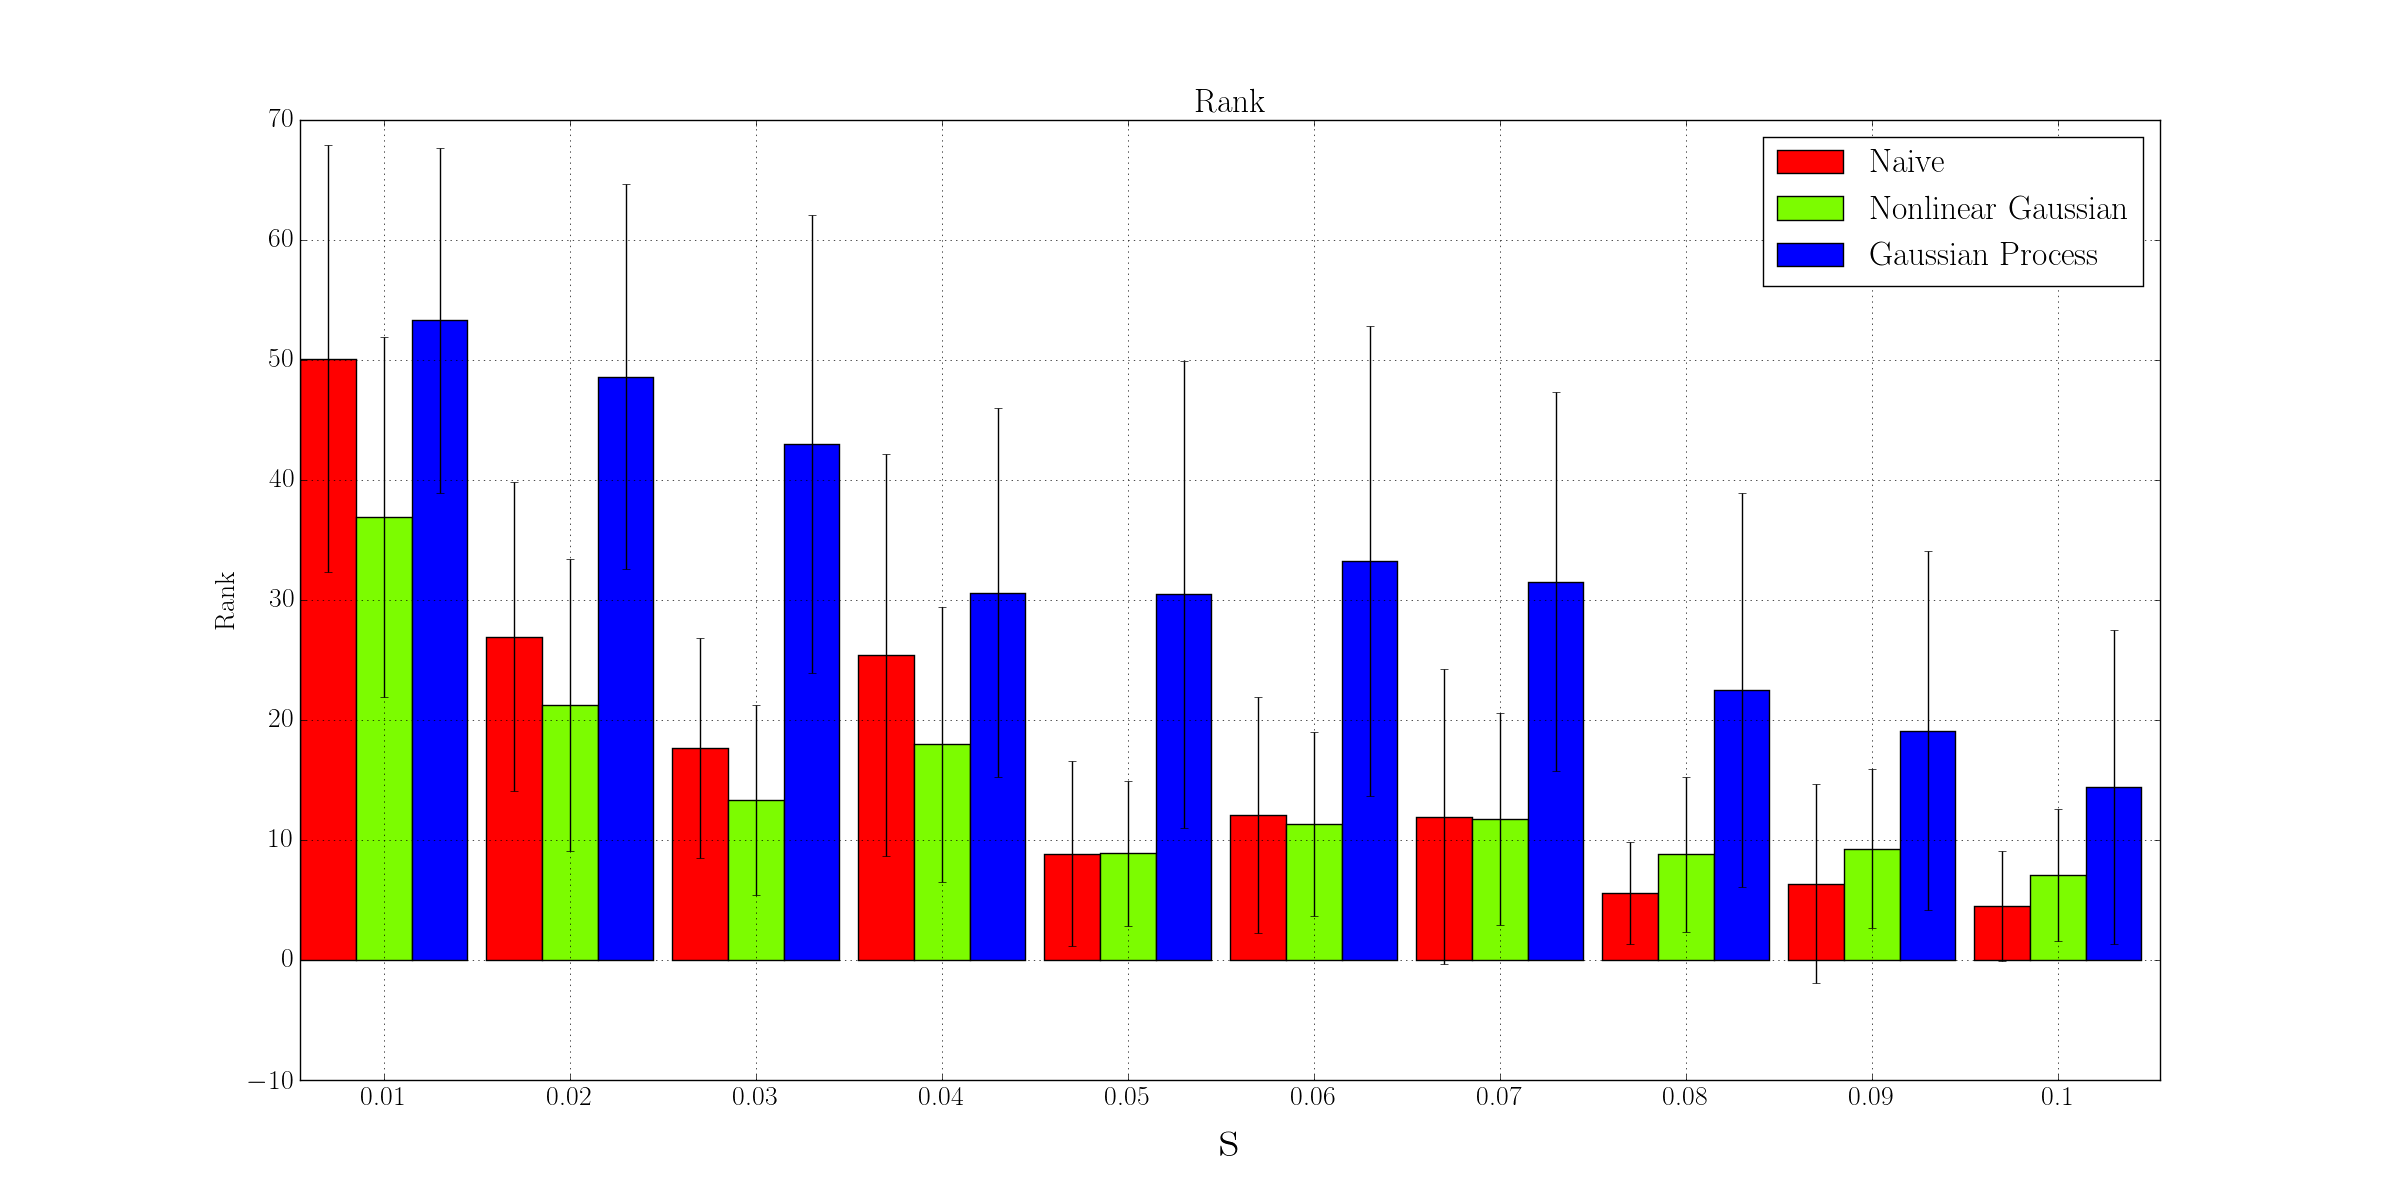
\includegraphics[width=\textwidth]{rank}
  \caption{Rank}
  \label{fig:Fig3}
\end{figure}

\paragraph{Mean Reciprocal Rank(MRR)}
\begin{figure}[H]
  \centering
    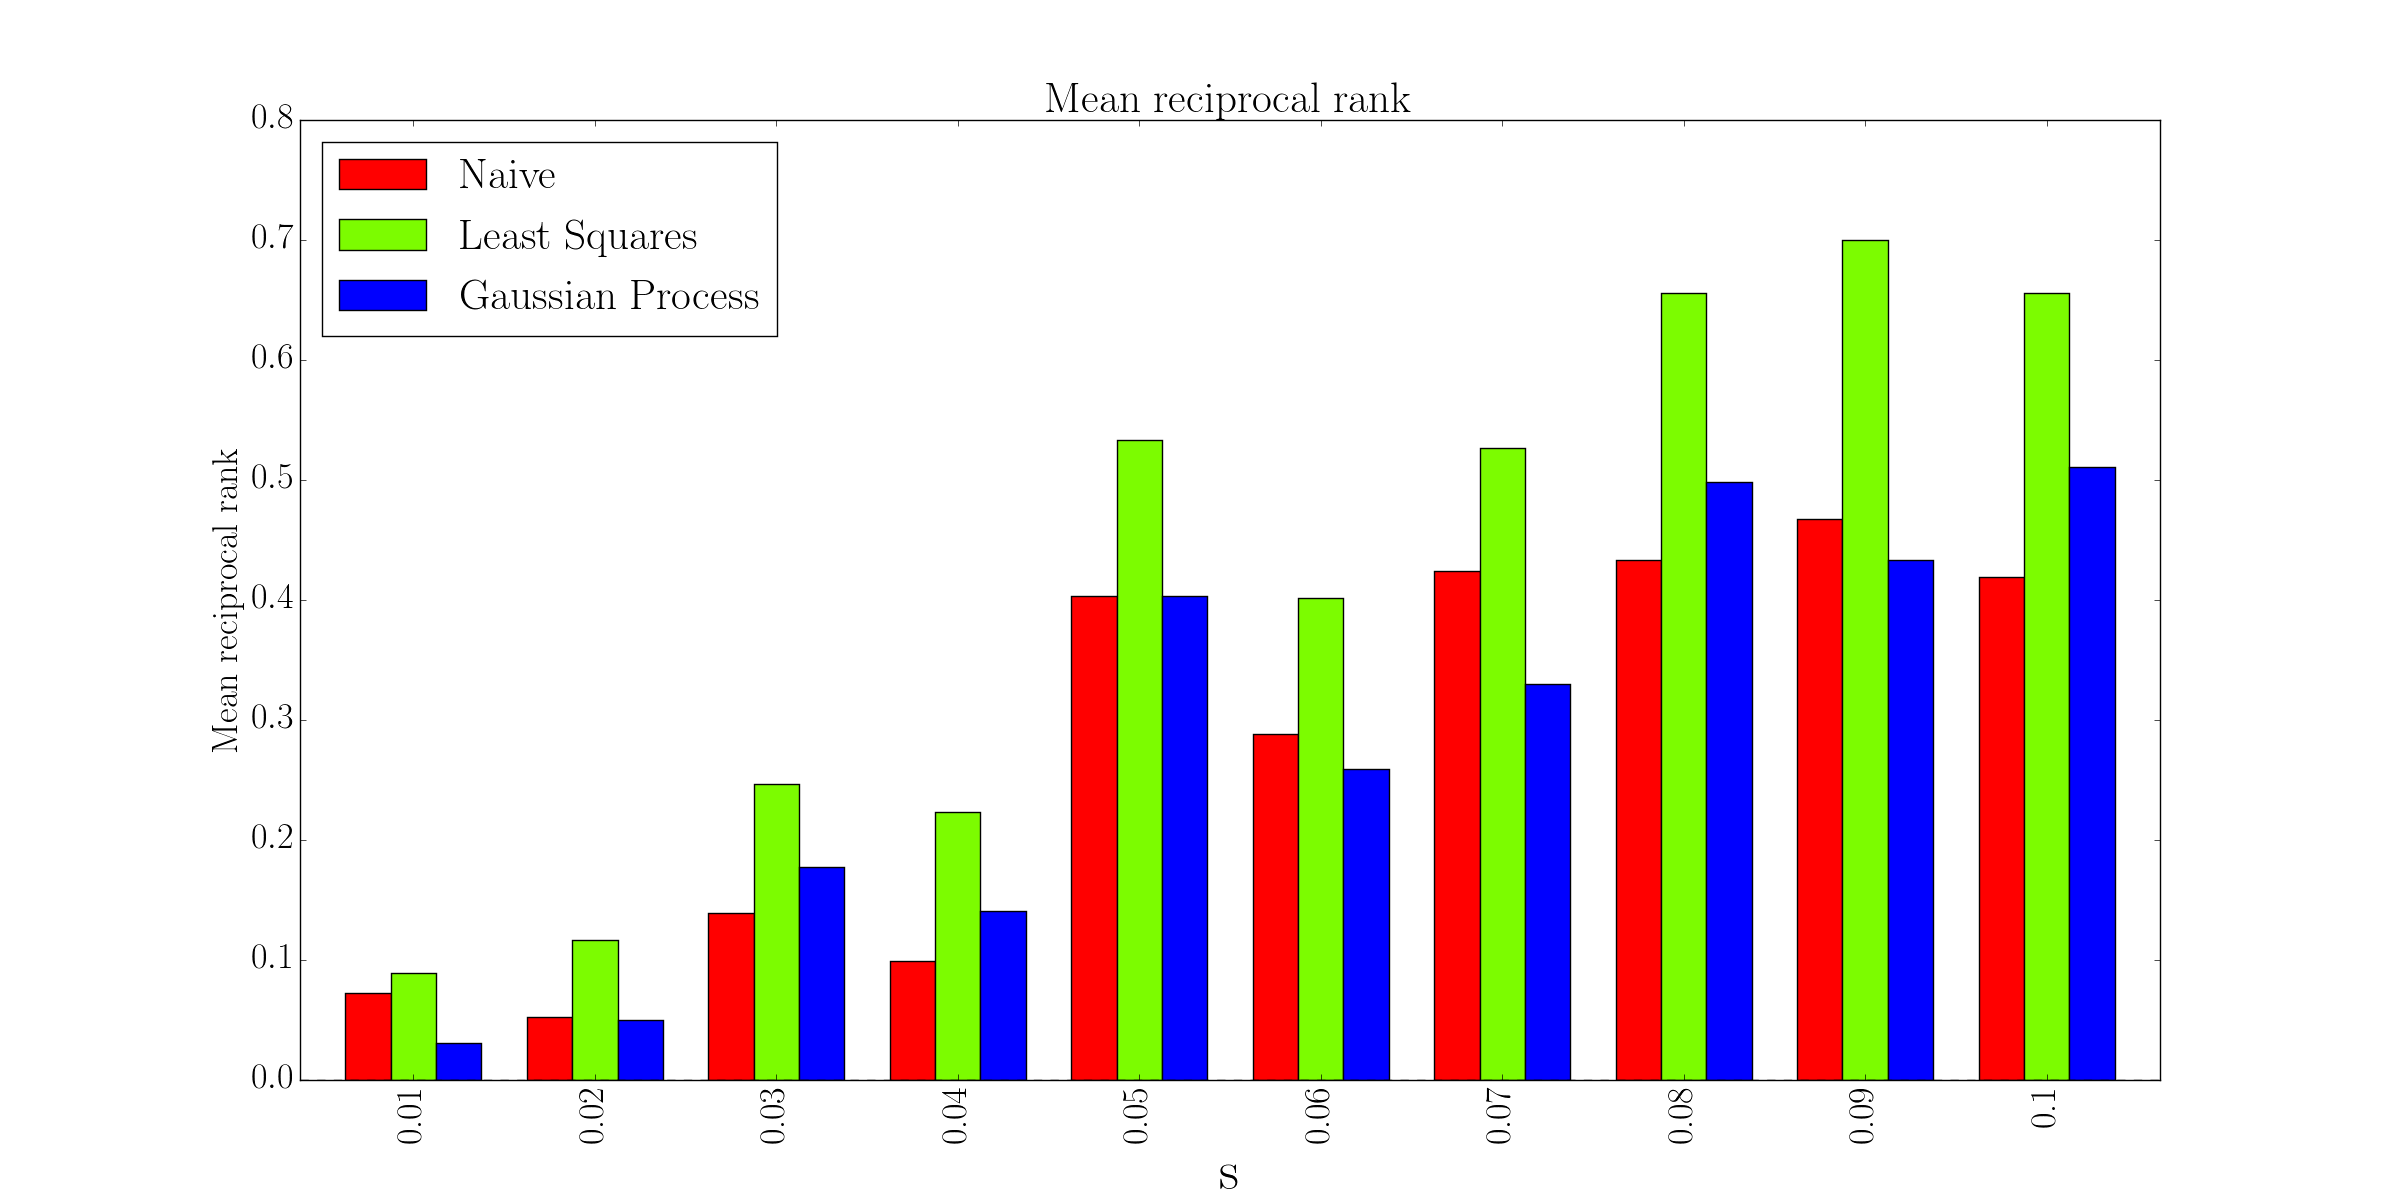
\includegraphics[width=\textwidth]{mrr}
  \caption{Mean Reciprocal}
  \label{fig:Fig2}
\end{figure}


\paragraph{Mean Average Precision (MAP)}
\begin{figure}[hh]
  \centering
    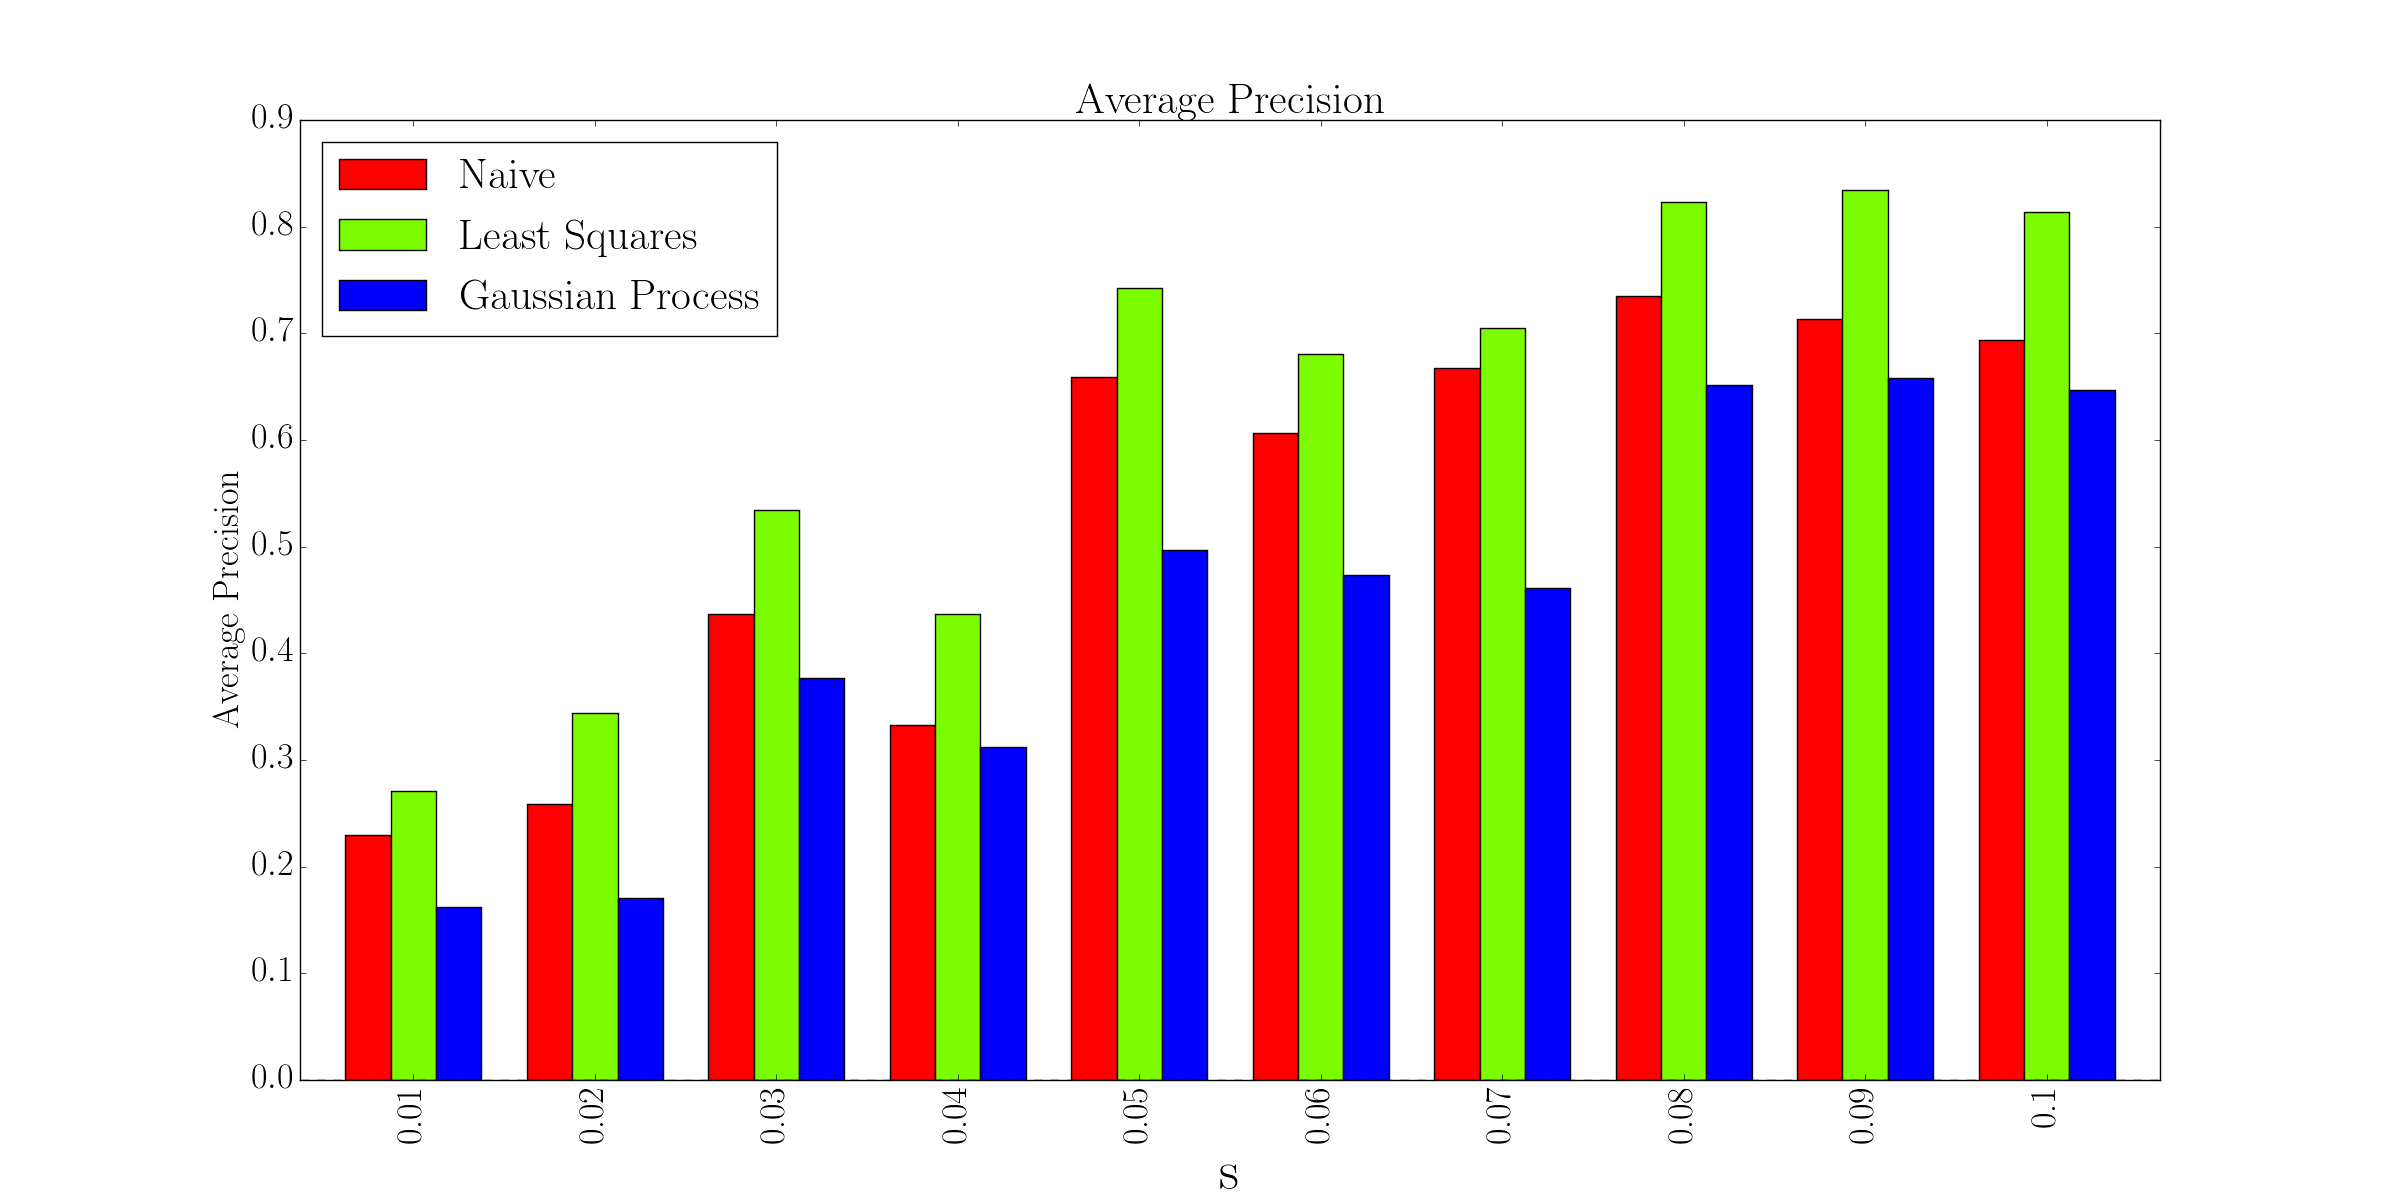
\includegraphics[width=\textwidth]{ap}
  \caption{Mean Average Precision (MAP)}
  \label{fig:Fig5}
\end{figure}


\subsubsection{Estimating Strength of Selection}
\begin{figure}[H]
  \centering
    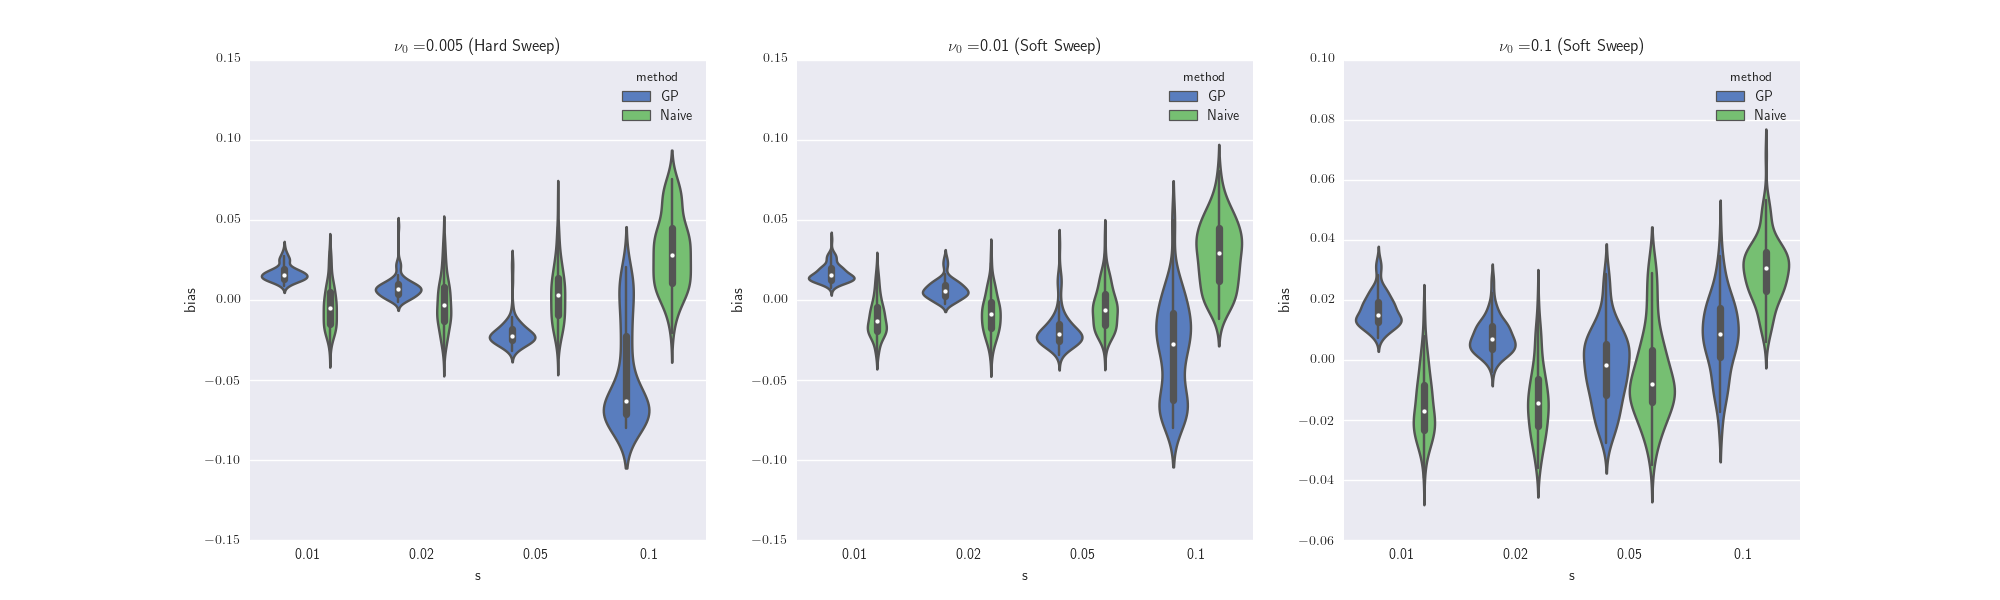
\includegraphics[width=\textwidth]{bias}
  \caption{Bias}
  \label{fig:Fig4}
\end{figure}

\subsection{Computational Performance}
%\section{Discussions}

%\newpage
%\bibliographystyle{acm}
%\bibliography{library}

%%%%%%%%%%%%%%%%%%%%%%%%%%%%%%%%%%%%%%%%%%%%%
%%%%%%%%%%%%%%%%%%% Supplemental Material%%%%
%%%%%%%%%%%%%%%%%%%%%%%%%%%%%%%%%%%%%%%%%%%%%
\clearpage
%\newpage
%\setcounter{page}{1}
\setcounter{figure}{0}
\setcounter{table}{0}
\setcounter{equation}{0}
\renewcommand{\thefigure}{S\arabic{figure}}
\renewcommand{\thetable}{S\arabic{table}}
\renewcommand{\theequation}{S\arabic{equation}}



\section{Appendix}
\subsection{Allele frequencies under selective sweep} \label{app:af}

\beq
\eeq
where $s\in \Rbb$ is the selection coefficient and $o\in[0,1]$ is the 
overdominance parameter which for $u=0.5$ we have
\begin{equation}
x_{t+1}=x_t+\frac{sx_t(1-x_t)}{2+2sx_t}\;.
\label{eq:transition}
\end{equation}
we also have
\beq
\frac{\bfd x_t}{\bfd t} = \frac{sx_t(1-x_t)}{2+2sx_t}
\eeq
which is a differential equation that is difficult to solve. However if take 
the approximation $2+2sx_t \approx 2$, it becomes an ordinary differential 
equation that can be readily solved

\begin{equation}
\nu_t =\frac{1}{1+\frac{1-x_0}{x_0}e^{-st/2}} = \sigma(st/2+\eta(x_0)) 
\label{eq:inf-pop}
\end{equation}
where$\sigma(.)$ is the logistic
function and $\eta(.)$ is logit function (inverse of the logistic function). 

\subsection{Logistic Model for Selection.}
As maximum likelihood for estimating $s$ using Markov chain is computationally 
expensive, here we use and logistic function for modeling allele frequencies 
undergoing selective sweep.
In a pure selection process with no drift, i.e. infinite 
population size, 
dynamic of allele frequencies 
can be well approximated by the logistic function (see 
Appendix \ref{app:af} 
for 
derivation)
\beq
\nu_t=\sigma(st+\eta(\nu_0))\label{eq:nut}
\eeq
where $\sigma(x)=1/(1+e^{-x})$ is the logistic function, and 
$\eta(x)=\log(x)/\log(1-x)$ is inverse of the 
logistic, aka logit, function. Figure \ref{fig:sweep} depicts 
the behavior of 
the logistic model for site allele frequencies and the 
default sampling time 
span(STS). Without genetic drift, soft sweep is easier to 
detect, 
because the logistic function happens to have steeper slope 
in th STS than 
those of hard sweeps, due to standing variation frequency. In addition, even 
under infinite 
population size regime, it is 
difficult differentiate between weak selections and genetic 
drift (a horizontal 
line), in short (e.g. 50 generations) experimental evolutions.


As shown in Figures \ref{fig:dynamic-weak} and \ref{fig:dynamic-strong} (first 
row), the approximate logistic model is consistent with 
simulated data and we 
use it to estimate the strength of selection for 
each site by solving a linear system of equations(see Section 
\ref{sec:regression} for details).

\subsection{Fay Wu's H}\label{app:h}
%\bl
In any finite population size of $n$ with $m$ segregating sites, 
allele frequencies take 
discrete values, i.e.,  $x_j \in 
\{\frac{1}{n},\frac{2}{n},\ldots,\frac{n-1}{n}\}, \ \forall j \in{1,\cdot,m}$ 
and we can write
\beq
\|\bfx\|^2= \sum_{j=1}^{m} x_j^2 = 
\sum_{i=1}^{n-1}\left(\frac{i}{n}\right)^2\xi_i= 
\frac{ (n-1)}{2n}H 
\eeq
where $\xi_i$ is the number of sites with frequency $i/n$ and $H$ is the 
Fay \& Wu's estimate of $\theta$.
%\el

Recently, Ronen et al. ~\cite{ronen2015predicting} devised the $1\dHAF$ 
statistic for identifying selection on static data, which has the expected 
value related to the $\|\bfx\|^2$:
\begin{equation} 
\Ebb[1\dHAF(t)]= n\| \bfx_t\|^2\approx ng(\nu_t)
\end{equation} 
where
\beq
g(\nu_t)= \theta \nu_t \left(\frac{\nu_t+1}{2} - \frac{1}{(1-\nu_t)n+1}\right) +
\theta (1-\nu_t)\left(\frac{n+1}{2n}-\frac{1}{(1-\nu_t)n+1}\right)
\label{eq:hafscorepooled}
\eeq
where easily follows that
\beq
\theta_H(t)=\frac{n-1}{2} g(\nu_t)
\eeq

\subsection{Tajima's D}\label{app:td}
Let $D_0, \Pi_0, W_0$, be Tajima's D, Tajima's estimate of  $\theta$, and 
Watterson's estimate of $\theta$ at time zero and $D_0=\Pi_0 - W_0$.
In order to compute, $D_t=\Pi_t - W_t$ we compute $\Pi_t$ and $W_t$ separately 
as follows.

Let $P$ be the $n \times n$ matrix of pairwise heterozygosity if individuals, 
then $\Pi=\frac{1}{n^2}\sum P_{ij}$. So, if the population consist of $\nu n$ 
identical carrier haplotype (due to lack of recombination), their pairwise 
hamming distance is zero and should be subtracted from the total $\Pi_t$:
\beq
\Pi_t&= (1-\nu_t^2)\Pi_0 
\eeq

To compute $W_t$, first remember that $W_t= \frac{m_t}{S_n}$ where $m_t$ is the 
number of segregating sites at time $t$ and $S_n= \sum_i^n 1/i \approx 
\log(n)$. Also we have
\beq
\frac{W_t}{W_0}&=\frac{\frac{m_t}{S}}{\frac{m_0}{S}} \ \ \Rightarrow 
W_t=\frac{m_t}{m_0}W0 
\eeq
where $m_t$ to be interpreted as the expected number of segregating sites at 
time $t$, under neutral evolution. At time $t$, the number of individuals that 
undergone neutral evolution is $(1-\nu_t)n +1$, which leads to
\beq
\frac{m_t}{m_0}&=\frac{\log\left((1-\nu_t)n +1 \right)\theta}{\log(n)\theta} 
\approx  
\frac{\log\left((1-\nu_t)n\right)}{\log(n)} = \frac{\log(1-\nu_t)+\log(n)}{\log(n)} = 
1+ \frac{ \log(1-\nu_t)}{\log(n)} 
\eeq
putting all together 
\beq
D_t&= (1-\nu_t^2)\Pi_0 - (1+ \frac{ \log(1-\nu_t)}{\log(n)} ) W_0 = 
D_0-\log(1-\nu_t) \frac{W_0}{\log(n)} -\nu_t^2 \Pi_0
\eeq


\subsection{Linkage Disequilibrium}
Nonrandom associations between polymorphisms are established in the 
substitution process according to the phylogeny, broken by recombination events 
and reinforced by selection. Although in EE the experiments with pooled 
sequencing, LD can not be measured throughout evolution, it is still worthwhile 
to examine the behavior of LD as a result of the interaction between 
recombination and natural selection, to take into account of some of EE 
implicit constraints. 

Let $\rho_0$ be the LD at time zero between the site under selection and a 
segregating site $l$ base-pairs away, then under natural selection we have
\beq
\rho_t= \alpha_t\beta_t \rho_0=e^{-rtl} \left(\frac{H_t}{H0}\right)  
\rho_0\label{eq:ldt}
\eeq
where $H_T=2\nu_0(1-\nu_0)$ is the heterozygousity at the selected site, $r$ is 
the recombination rate/bp/gen. The decay factor $\alpha_t=e^{-rtl}$ is the 
product of recombination and growth factor $\beta_t$ (eq. 30-31 in 
\cite{Stephan2006The})is the outcome of 
selection. For $s=0.01$, $l=100K$bp, the log of decay, growth and product of 
both is depicted in Figure \ref{fig:ldf}. It is evident that, for these 
parameters LD does not start to decay until generation 1000, which would be  
problematic when $\rho_0$. For example, in the case of hard sweep, the 
selection is imposed on the site with minimum AF, which is at perfect linkage 
($|D'|=1$) with all the other loci.\footnote{This is because, between the 
	selected site and all the other sites frequency of one gamete is zero.}
We this phenomenon is shown in the Figures \ref{fig:ld2d}, \ref{fig:ld3d} where 
at generation zero the site at position 500K is at perfect linkage with all the 
other sites, and linkage of the middle site with all the genome is depicted 
for both genetic drift and natural selection, in different generations.
Also, a window of 50Kbp around the selected site is shaded in Figure 
\ref{fig:ld2d} to demonstrate the value of LD in the window under drift and 
hard sweep. This implies that the precision of locating the selection on the 
genome is tightly dependent on a set of parameters including, recombination 
rate, selection strength, initial carrier frequency, and the initial linkage.
\subsection{Likelihood Functions} \label{app:likelihood}
Actually, it is enough to show \eqref{eq:transition} is
linear fractional in $s$, which is nby definition: linear numerator
and denominator, and strictly positive denominator.
\clearpage
\newpage

\section{Supplemental Figures and Tables}

\begin{figure}[H]
	\centering
	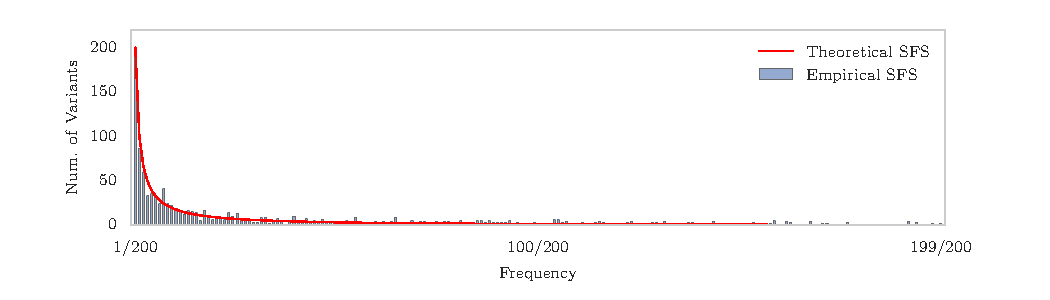
\includegraphics[trim=1in 0.1in 1in 0.1in,clip,width=\textwidth]{figures/sfs.pdf}
	\caption{Theoretical and Empirical SFS for a neutral population of 200 
	individuals.}	\label{fig:sfs}
\end{figure}

\begin{figure}[H]
	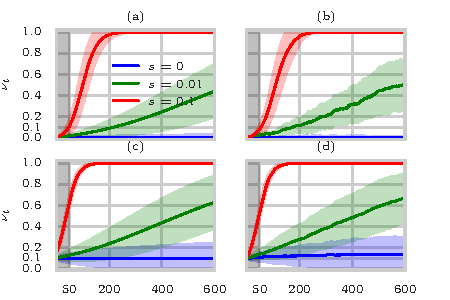
\includegraphics[trim=0in 0.1in 1in 0.1in,clip,width=\textwidth]{figures/AF.pdf}
	\caption{Logistic model for different selection strengths 
		for soft (left) 
		and hard (right) sweep as a function of time in 
		generations. The first 
		50 
		generations, which observations are sampled is 
		shaded.} 	 
	\label{fig:sweep}
\end{figure}
\begin{figure}[H]
	\centering
	\includegraphics[trim={0in 0.1in 0in 
		0in},clip,width=\textwidth]{figures/{tdterms}.png}
	\caption{Interactions of two terms in $D$. W.l.o.g when $D_0=0$ and 
	$\Pi_0=W_0=1$, 
		$D_t$ is sum of the 
		logarithmic $\frac{-\log(1-\nu_t)}{\log(2N)}$ and the squared term 
		$\nu_t^2$.} 	 
	\label{fig:tdterms}
\end{figure}

\begin{figure}[H]
	\centering 
	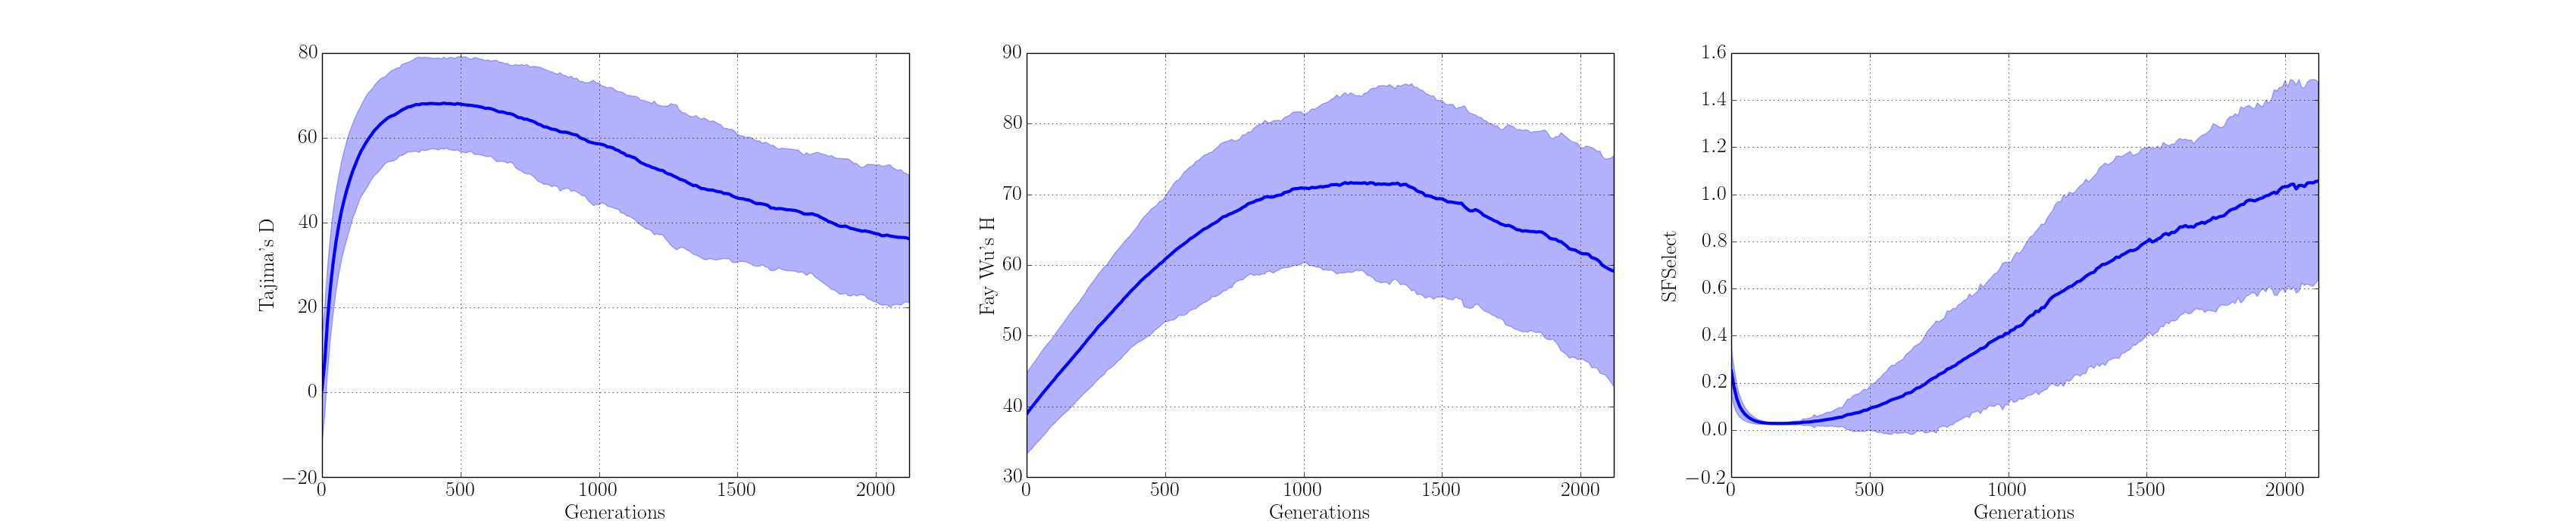
\includegraphics[trim=3.2in 0.1in 3.2in 0.2in , 
	clip,width=\textwidth]{figures/bottleneck}
	\caption{Effect of bottle neck in a typical experimental evoloution 
		experiment where a restricted number of founder lines (here $F=200$) is 
		selected out of a larger population size ($N_e=10^{-6}$). Tajima's D 
		(left), Fay Wu's H (middle) and SFSelect is computed for 1000 neutral 
		simulations and mean and 95\% confidence interval is plotted.} 
	\label{fig:bottleneck}
\end{figure}

\begin{figure}[H]
	\centering 
	\includegraphics[width=\textwidth]{figures/{msmsts}.pdf}
	\caption{Mean and 95\% CI of 1000 simulations for neutral (blue trajectories) selection with $s=0.1$ (red trajectories).}
	\label{fig:sfsts}
\end{figure}



\begin{figure}[H]
	\centering
	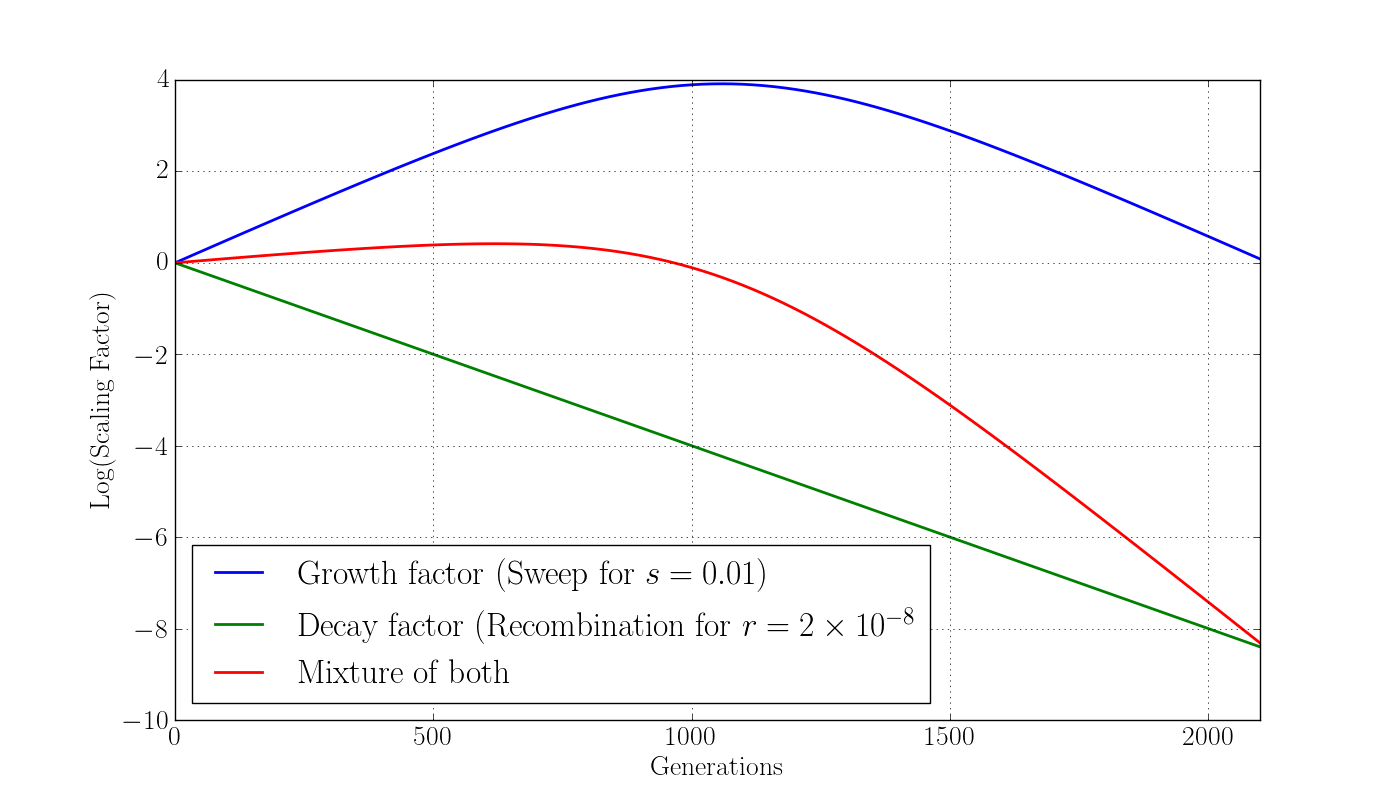
\includegraphics[width=\textwidth]{figures/decayFactors}
	\caption{Interaction between productive factors of LD under natural 
		selection for weak selection (s=$0.01$) and a distance of 100Kb between 
		sites. In this setting, after about 1000 generations LD start to decay 
		(red 
		curve).} \label{fig:ldf}
\end{figure}


\begin{figure}[H]
	\centering
	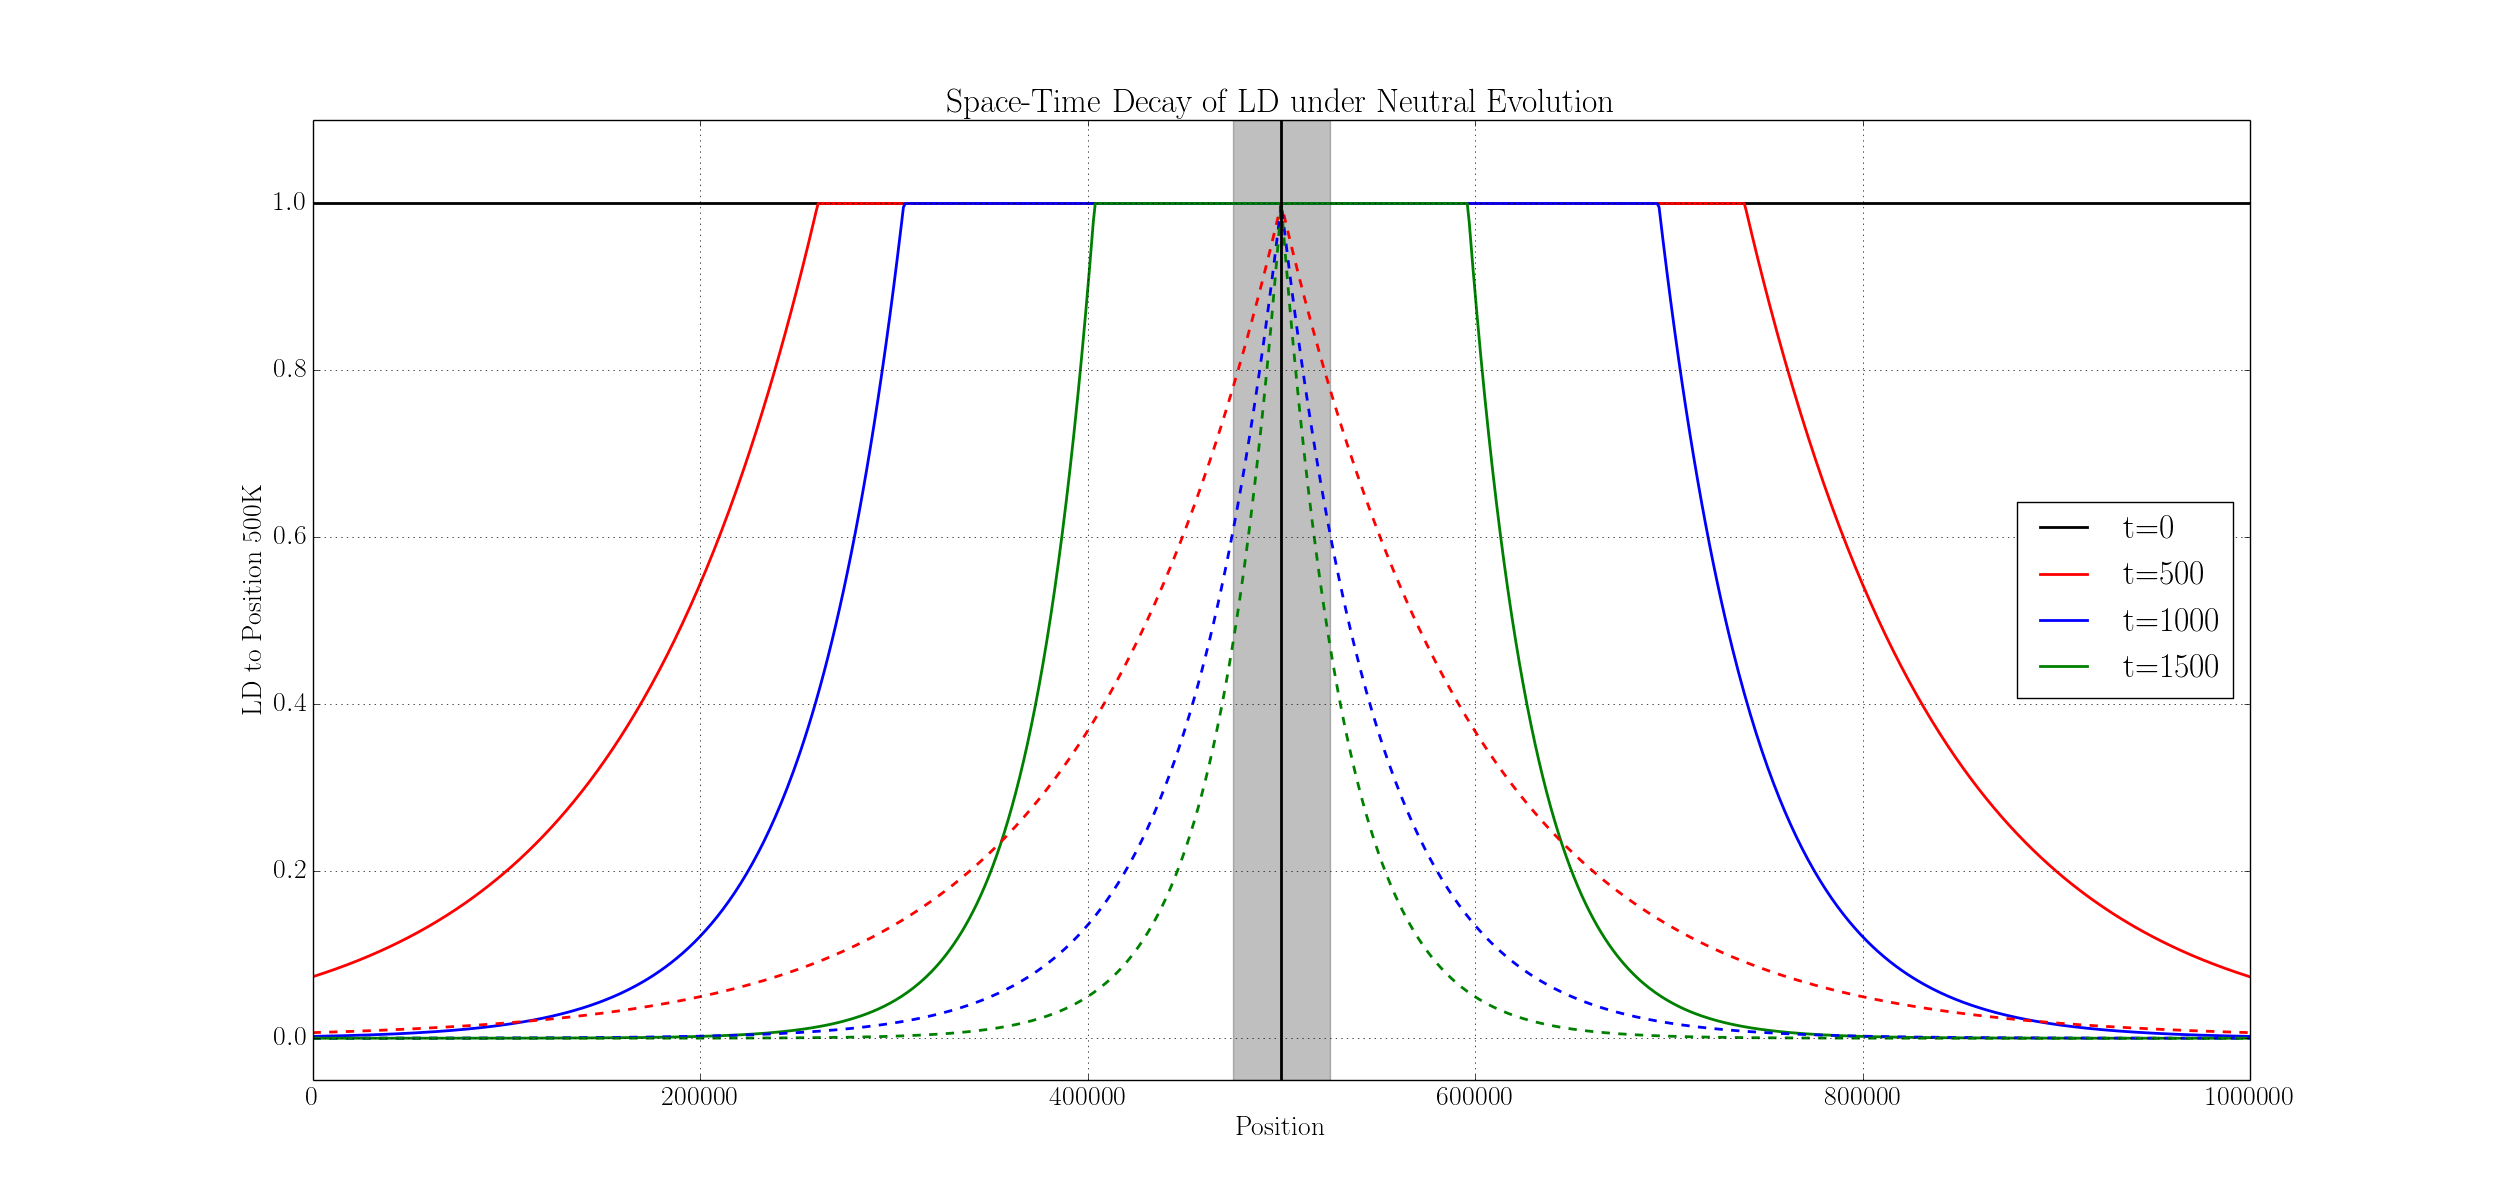
\includegraphics[width=\textwidth]{figures/LDDecay2d}
	\caption{Decay of LD ($|D'|$ measure) of the minimum AF site at position 
		500K with the rest of genome when $s=0.01$ and $r=2\times10^{-8}$. A 
		window 
		of 50Kb is shaded at the center of genome to illustrate high values of 
		linkage in both selection and drift.} \label{fig:ld2d}
\end{figure}


\begin{figure}[H]
	\centering
	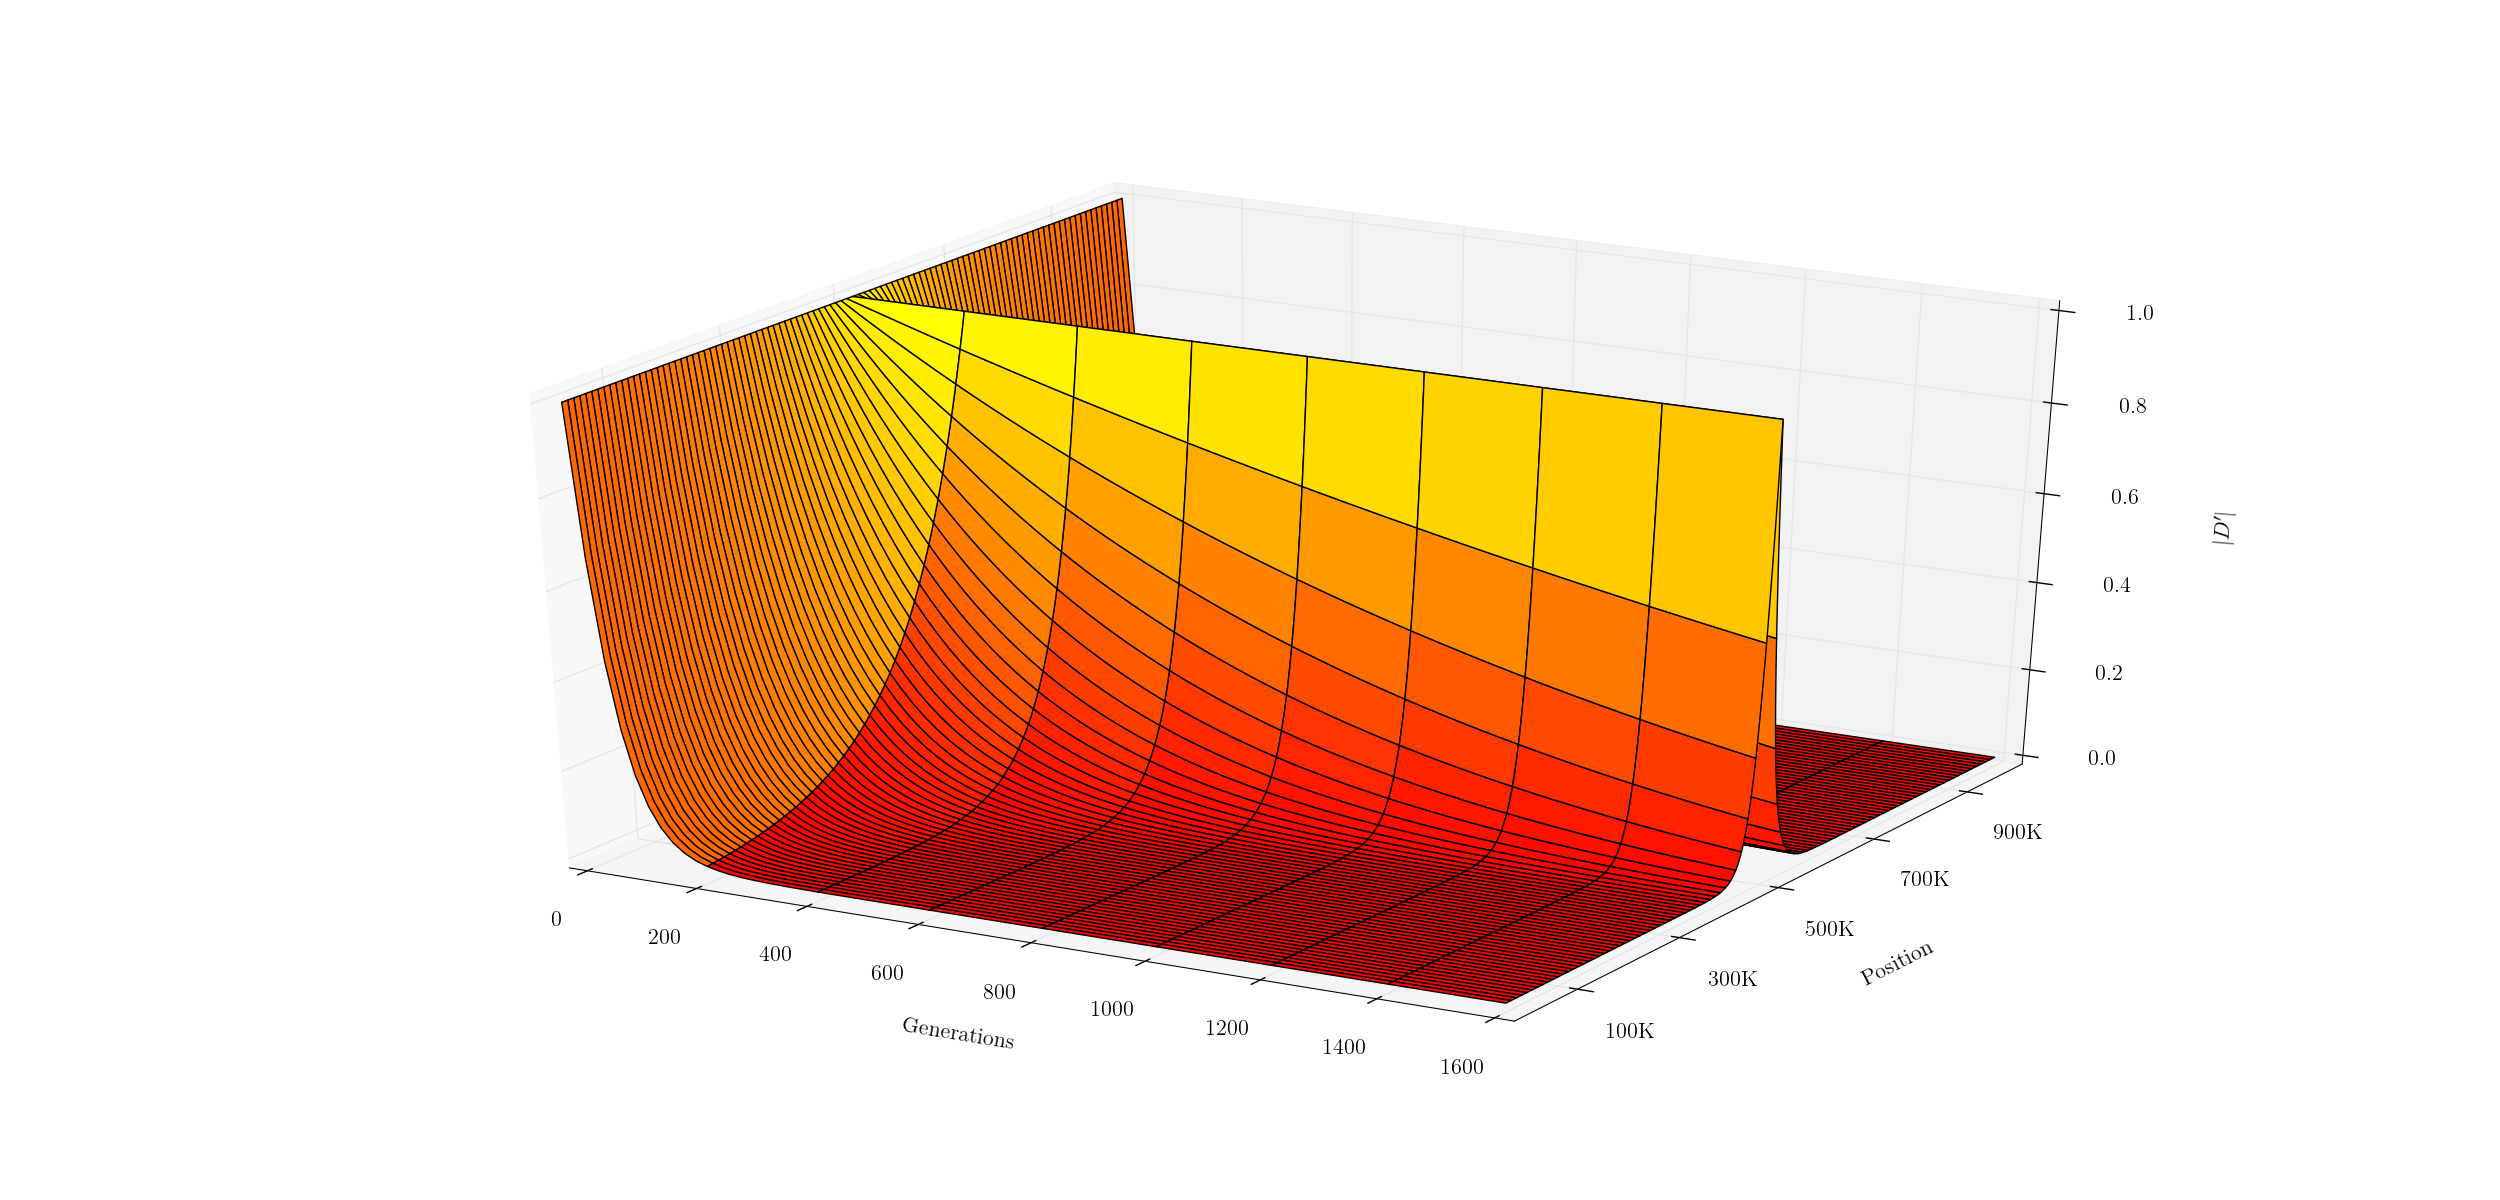
\includegraphics[width=\textwidth]{figures/LDDecay3dNeutral}
	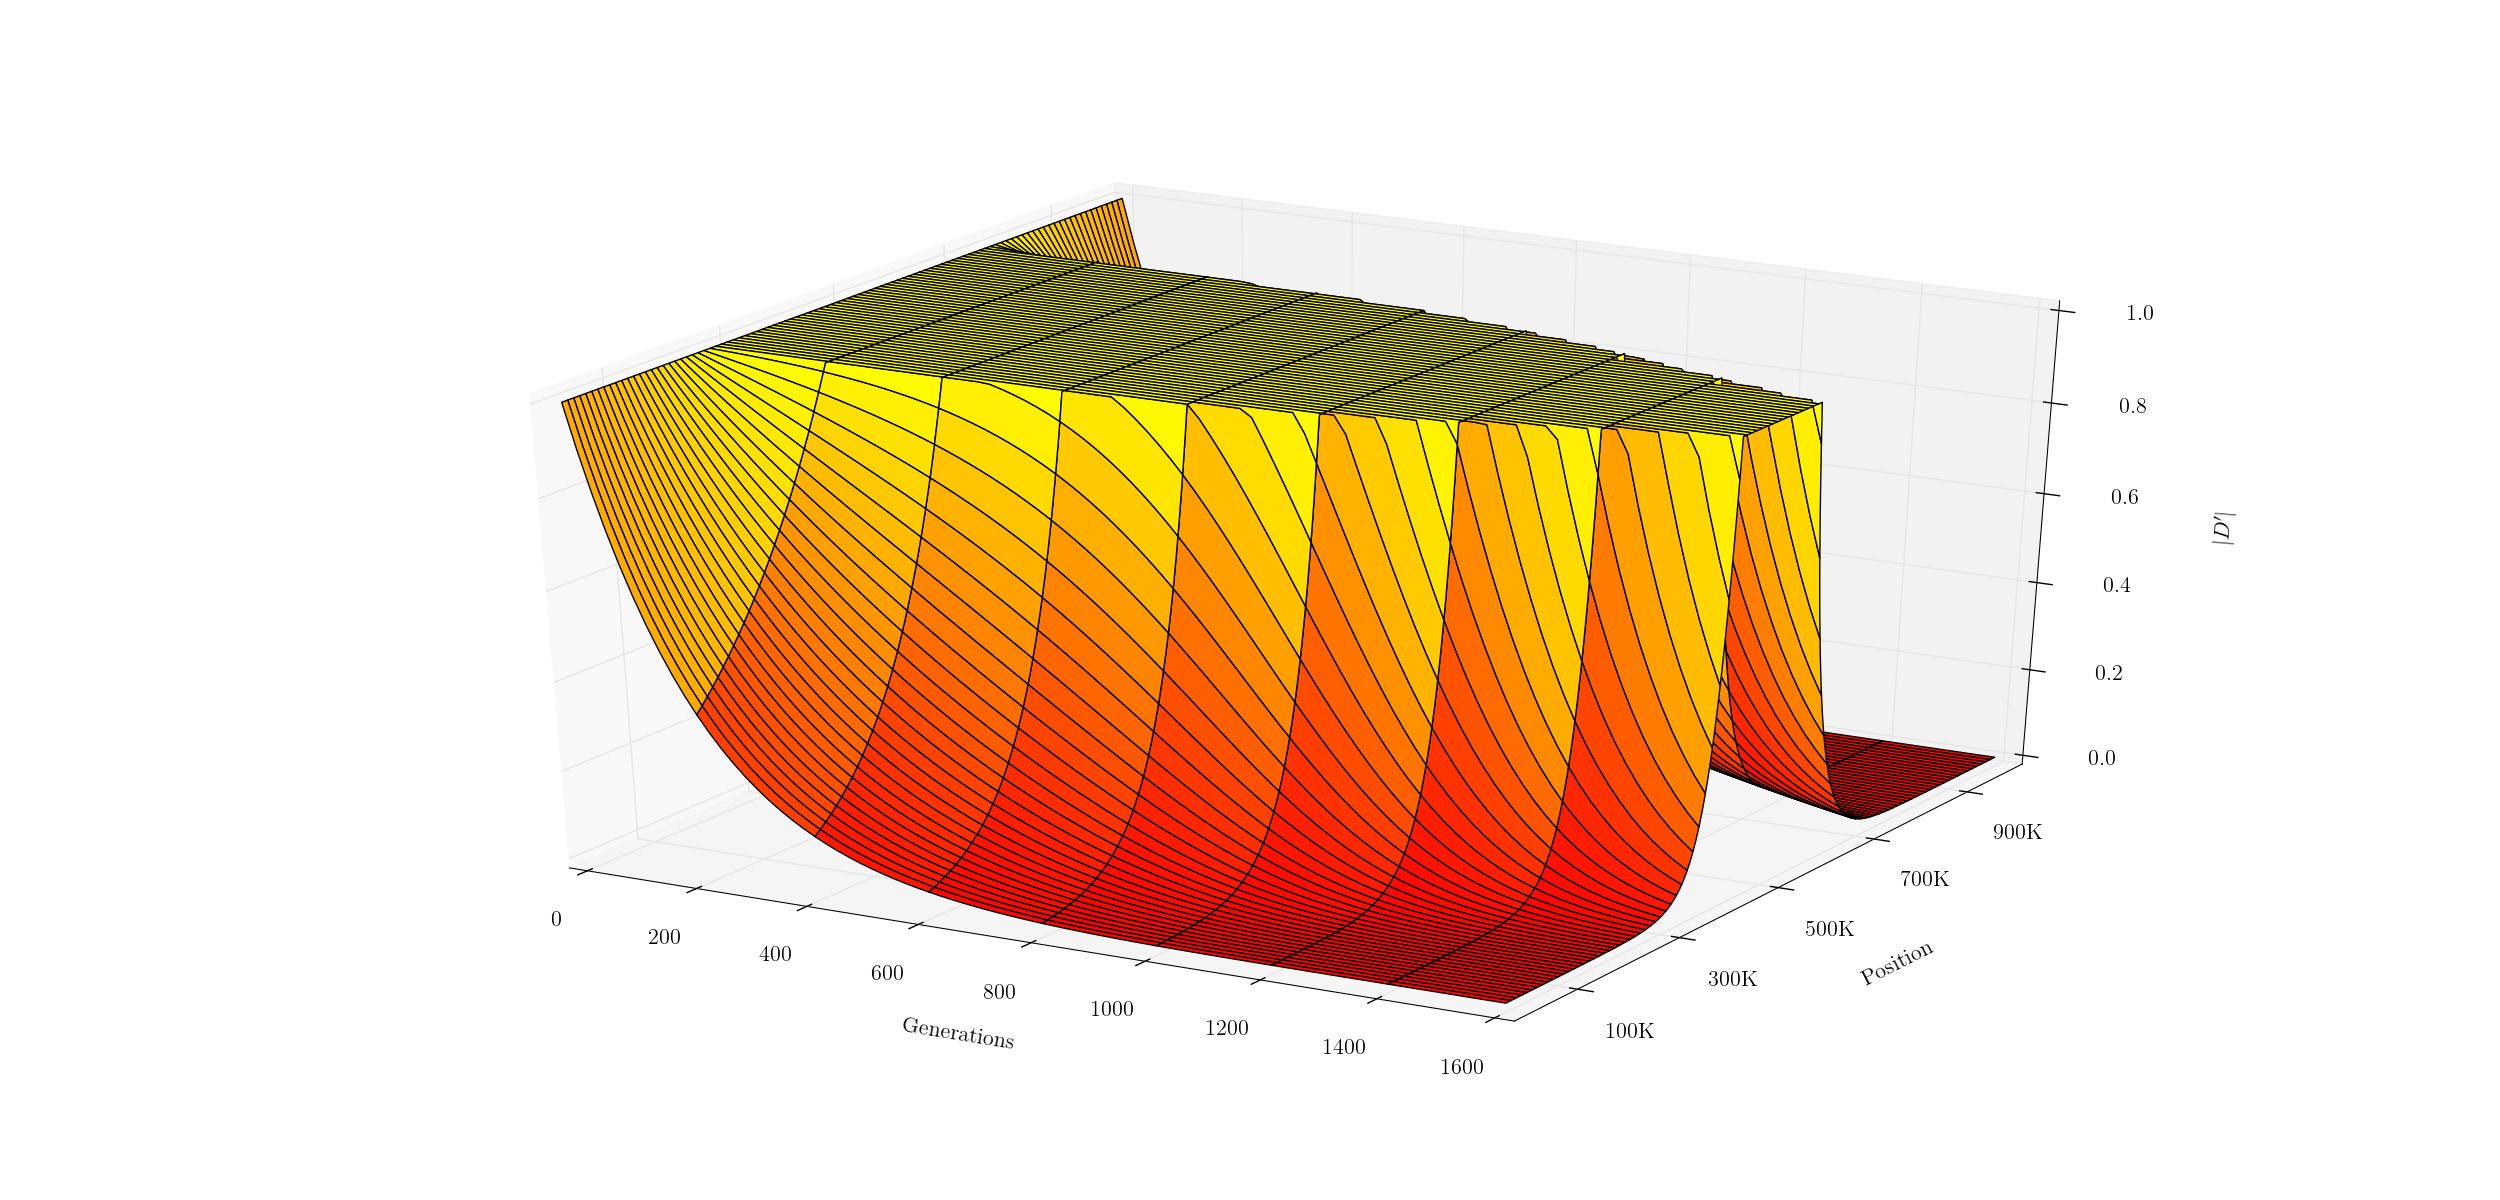
\includegraphics[width=\textwidth]{figures/LDDecay3dSweep}
	\caption{ld} \label{fig:ld3d}
	\caption{Decay of LD ($|D'|$ measure) of the minimum AF site at 
		position 500K with the rest of genome in genetic drift with 
		$r=2\times10^{-8}$ (top) and hard sweep with $s=0.01$ (bottom).}
\end{figure}




\begin{figure}[H]
	\centering
	\includegraphics[trim=1.2in 0 .0in 0, 
	clip,width=\textwidth]{figures/{dominance}.png}
	\caption{Dominance for $s=0.1$.} 
	\label{fig:dominance}
\end{figure}

\begin{figure}[H]
	\centering
	\includegraphics[trim=.2in 0 .0in 0, 
	clip,width=\textwidth]{figures/{qq}.pdf}
	\caption{QQ plot for a simulation.} 
	\label{fig:qq}
\end{figure}



\begin{figure}[H]
	\centering
	\includegraphics[trim=.0in 0 .0in 0, 
	clip,width=\textwidth]{figures/{samplingTimes}.pdf}
	\caption{sampling times.} 
	\label{fig:samplingTimes}
\end{figure}



\begin{figure}[H]
	\centering
	\includegraphics[trim=.0in 0 .0in 0, 
	clip,width=0.5\textwidth]{figures/{statePosterior}.pdf}
	\caption{Posterior distribution of allele frequencies (states), for 
	different values of depth $d=\{5,50,500\}$. In all the cases, the number of 
	read counts for the derived allele is one-fifth of total depth. Dealing 
	with dynamic data (and possibly multi-replicate), each site has multiple 
	measurements, that can have different depth, i.e. uncertainty.} 
	\label{fig:stateConditional}
\end{figure}


\begin{figure}[H]
	\centering
	\begin{tabular}{ccc}
				\includegraphics[trim=.1in 0 .0in 0, 
				clip,width=0.3\textwidth]{figures/{Song}.pdf} &
		\includegraphics[trim=.1in 0 .0in 0, 
		clip,width=0.3\textwidth]{figures/{BM}.pdf} &
		\includegraphics[trim=.1in 0 .0in 0, 
		clip,width=0.3\textwidth]{figures/{BF}.pdf}
	\end{tabular}
	\caption{Song, HSF, HSP.} 
	\label{fig:geneRanking}
\end{figure}


\begin{figure}[H]
	\centering
	\begin{tabular}{c}
		\includegraphics[trim=.2in 0 .0in 0, 
		clip,width=\textwidth]{figures/{depth}.pdf}
	\end{tabular}
	\caption{Scaled PDF (left) and CDF (right) of the overall read depth distribution (top) and minimum depth of sites (bottom).
		Top row depicts the overall distribution of rad of all reads.} 
	\label{fig:depth}
\end{figure}

\begin{figure}[H]
	\centering
	\begin{tabular}{c}
		\includegraphics[trim=.2in 0 .0in 0, 
		clip,width=\textwidth]{figures/{depthHetero}.pdf}
	\end{tabular}
	\caption{Read depth at four different sites. (which would be filtered if the min depth is set to 30X)} 
	\label{fig:depthHetero}
\end{figure}


\begin{table}[h]
	\begin{tabular}{c||c}
		Hard Sweep & Soft Sweep\\ \\  
		\centering \begin{tabular}{c|c|c|c}
$\lambda$	&$\pi$	&LR	&Avg Power\\\hline
300	&98	&	&42\\
300	&99	&	&42\\
300	&95	&	&41\\
300	&96	&	&41\\
300	&97	&	&41\\
300	&90	&	&40\\
300	&96	&+	&39\\
300	&97	&+	&39\\
300	&98	&+	&39\\
300	&99	&+	&39\\
300	&50	&	&39\\
300	&95	&+	&38\\
300	&90	&+	&36\\
300	&100	&	&36\\
300	&100	&+	&32\\
300	&0	&+	&31\\
300	&50	&+	&31\\
300	&0	&	&16\\
100	&96	&	&40\\
100	&97	&	&40\\
100	&98	&	&40\\
100	&95	&	&39\\
100	&90	&	&38\\
100	&99	&	&38\\
100	&50	&	&35\\
100	&0	&+	&29\\
100	&50	&+	&29\\
100	&90	&+	&27\\
100	&95	&+	&27\\
100	&96	&+	&27\\
100	&97	&+	&27\\
100	&98	&+	&26\\
100	&99	&+	&25\\
100	&100	&	&24\\
100	&100	&+	&16\\
100	&0	&	&8\\
30	&90	&	&28\\
30	&95	&	&28\\
30	&96	&	&28\\
30	&97	&	&27\\
30	&98	&	&26\\
30	&50	&	&25\\
30	&99	&	&23\\
30	&0	&+	&22\\
30	&50	&+	&20\\
30	&90	&+	&13\\
30	&95	&+	&10\\
30	&96	&+	&10\\
30	&100	&	&10\\
30	&97	&+	&9\\
30	&98	&+	&9\\
30	&99	&+	&7\\
30	&100	&+	&6\\
30	&0	&	&3\\
\end{tabular}

				&\centering \begin{tabular}{c|c|c|c|c}
$\lambda$	&$\pi$	&LR	&Method	&Avg Power\\\hline
$\infty$	&100	&	&$\mathcal{M}$	&73\\
$\infty$	&100	&+	&$\mathcal{M}$	&72\\
$\infty$	&99	&+	&$\mathcal{M}$	&70\\
$\infty$	&99	&	&$\mathcal{M}$	&69\\
$\infty$	&50	&	&$\mathcal{M}$	&64\\
$\infty$	&50	&+	&$\mathcal{M}$	&63\\
$\infty$	&0	&+	&$\mathcal{M}$	&63\\
$\infty$	&0	&	&$\mathcal{M}$	&46\\\hline
100	&99	&+	&$\mathcal{H}$	&65\\
100	&99	&	&$\mathcal{H}$	&65\\
100	&99	&	&$\mathcal{M}$	&65\\
100	&50	&+	&$\mathcal{H}$	&64\\
100	&0	&+	&$\mathcal{H}$	&64\\
100	&50	&	&$\mathcal{H}$	&64\\
100	&50	&+	&$\mathcal{M}$	&62\\
100	&0	&+	&$\mathcal{M}$	&62\\
100	&100	&	&$\mathcal{H}$	&62\\
100	&50	&	&$\mathcal{M}$	&62\\
100	&100	&+	&$\mathcal{H}$	&61\\
100	&100	&	&$\mathcal{M}$	&61\\
100	&99	&+	&$\mathcal{M}$	&58\\
100	&100	&+	&$\mathcal{M}$	&54\\
100	&0	&	&$\mathcal{H}$	&42\\
100	&0	&	&$\mathcal{M}$	&25\\\hline
30	&50	&+	&$\mathcal{H}$	&58\\
30	&0	&+	&$\mathcal{H}$	&58\\
30	&50	&	&$\mathcal{H}$	&57\\
30	&99	&	&$\mathcal{H}$	&53\\
30	&99	&+	&$\mathcal{H}$	&51\\
30	&99	&	&$\mathcal{M}$	&48\\
30	&50	&+	&$\mathcal{M}$	&47\\
30	&0	&+	&$\mathcal{M}$	&47\\
30	&100	&	&$\mathcal{H}$	&47\\
30	&50	&	&$\mathcal{M}$	&47\\
30	&100	&+	&$\mathcal{H}$	&46\\
30	&100	&	&$\mathcal{M}$	&38\\
30	&99	&+	&$\mathcal{M}$	&34\\
30	&100	&+	&$\mathcal{M}$	&25\\
30	&0	&	&$\mathcal{H}$	&14\\
30	&0	&	&$\mathcal{M}$	&6\\
\end{tabular}

	\end{tabular}
	\caption{Average power, average true-positive-rate when FDR$\le$0.05, for 
	detecting selection in a 50Kbp region for Frequency Increment Test (FIT), 
	Gaussian Process (GP), Markov Chain ($\Mc$), Hidden Markov Model ($\Hc$) on 
	1000 
		simulations for each of selection strength $s$ and initial 
		carrier frequency $\nu_0$. To incorporate ascertainment bias, each 
		setting is evaluated such that depth of each SNP is identically 
		distributed from Poisson$(\lambda)$ for $\lambda \in 
		\{30,100,\infty\}$.}\label{tab:powerCLR}
\end{table}

\begin{table}[h]
	\centering
	\begin{tabular}{ccc}
		Hard Sweep & &Soft Sweep\\ \\  
		\centering \begin{tabular}{c|c|c}
$\lambda$	&Method	&Avg Power\\\hline
100	&$\mathcal{H}$	&30\\
$\infty$	&$\mathcal{H}$	&29\\
30	&$\mathcal{H}$	&23\\
100	&CMH	&19\\
30	&CMH	&10\\
$\infty$	&GP	&7\\
100	&GP	&7\\
30	&GP	&7\\
$\infty$	&FIT	&5\\
100	&FIT	&4\\
30	&FIT	&3\\
\end{tabular}

		&&\centering \begin{tabular}{c|c|c}
$\lambda$	&Method	&Avg Power\\\hline
100	&$\mathcal{H}$	&64\\
$\infty$	&$\mathcal{H}$	&63\\
$\infty$	&GP	&60\\
100	&GP	&60\\
100	&CMH	&59\\
30	&$\mathcal{H}$	&58\\
30	&GP	&56\\
30	&CMH	&44\\
$\infty$	&FIT	&36\\
100	&FIT	&21\\
30	&FIT	&7\\
\end{tabular}

	\end{tabular}
	\caption{Average power, average true-positive-rate when FDR$\le$0.05, for 
		detecting selection in a 50Kbp region for Frequency Increment Test 
		(FIT), 
		Gaussian Process (GP), Markov Chain ($\Mc$), Hidden Markov Model 
		($\Hc$) on 
		1000 
		simulations for each of selection strength $s$ and initial 
		carrier frequency $\nu_0$. To incorporate ascertainment bias, each 
		setting is evaluated such that depth of each SNP is identically 
		distributed from Poisson$(\lambda)$ for $\lambda \in 
		\{30,100,\infty\}$.}\label{tab:power}
\end{table}


\begin{figure}[H]
	\centering
	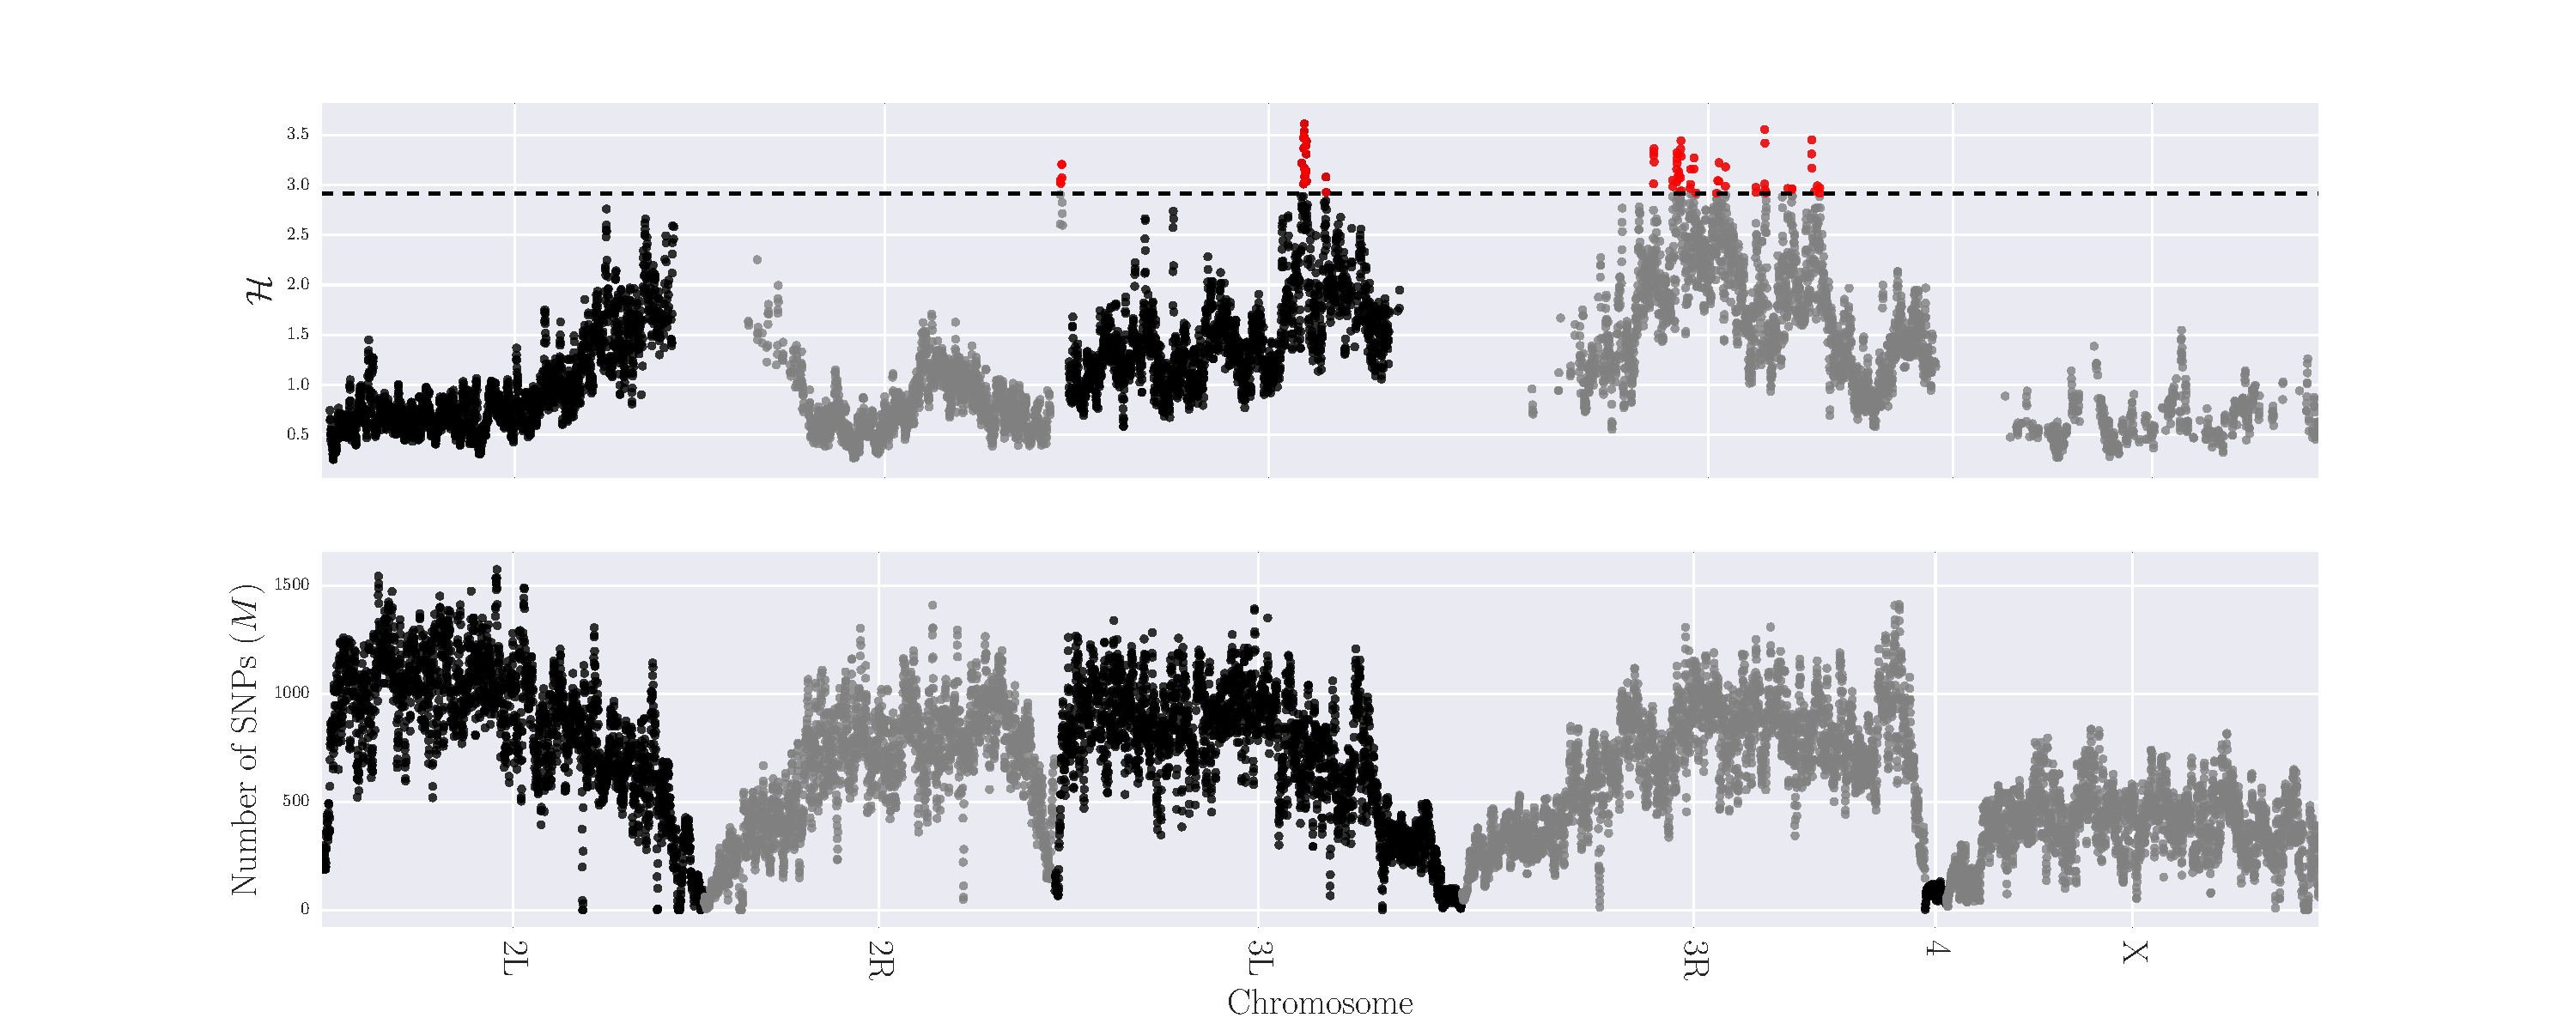
\includegraphics[width=\textwidth]{figures/manhattan.pdf}
	\caption{Manhattan plot of the composite $\Hc$ statistic (top) 
	and the number of SNPs (bottom) in 50Kbp sliding window with steps of 
	10Kbp. Regions in which their $\Hc$ statistic falls in top one percentile 
	distribution is denoted with red color. Pearson correlation between $M$ and 
	$\Hc$ of all windows is -0.03 and for the candidate regions is -0.27. This 
	nine-fold increase in correlation implies that the $\Hc$ statistic takes 
	more extreme values as the number of SNPs in the window is less than 
	expected ($\approx$1100).} 
	\label{fig:manhattan}
\end{figure}




%\begin{figure}[H]
%	\centering
%	\begin{tabular}{c}
%		\includegraphics[trim=.2in 0 .0in 0, 
%		clip,width=\textwidth]{figures/{siteDepthDist}.pdf}\\
%	\end{tabular}
%	\caption{Distribution of the mean and variance of the minimum depth of all sites.} 
%	\label{fig:siteDepthDist}
%\end{figure}
\newpage
\bibliographystyle{acm}
\bibliography{library}
\newpage
\end{document}
